% $Author: Luc $
% $Date: 2008-11-09 11:14:31 +0200 (Sun, 09 Nov 2008) $
% $Revision:  $
%=================================================================
\ifx\wholebook\relax\else
% --------------------------------------------
% Lulu:
    \documentclass[a4paper,10pt,twoside]{book}
    \usepackage[
        papersize={6in,9in},
        hmargin={.75in,.75in},
        vmargin={.75in,1in},
        ignoreheadfoot
    ]{geometry}
    % $Author$ Martial
% $Date$ Wed Oct 10 13:34:55 CEST 2007
% $Revision$ source: SBE 12715 
% Last Changed Date: 2007-10-08 21:32:45 +0200 (Mon, 08 Oct 2007)
%=============================================================
% NB: documentclass must be set in main document.
% Allows book to be generated in multiple formats.
%=============================================================
%:Packages
%\usepackage[french]{babel}
\usepackage[T1]{fontenc}  %%%%%% really important to get the code directly in the text!
\usepackage{lmodern}
%\usepackage[scaled=0.85]{bookmanx} % needs another scale factor if used with \renewcommand{\sfdefault}{cmbr}
\usepackage{palatino}
%\usepackage[sc]{mathpazo}
%\linespread{1.05}
\usepackage[scaled=0.85]{helvet}
\usepackage{microtype}
\usepackage{graphicx}
\usepackage{theorem}
\usepackage[utf8]{inputenc}
% ON: pdfsync breaks the use of p{width} for tabular columns!
\ifdefined\usepdfsync\usepackage{pdfsync}\fi % Requires texlive 2007
%=============================================================
%:More packages
%Stef should check which ones are used!
%\usepackage{picinpar}
%\usepackage{layout}
%\usepackage{color}
%\definecolor{stefgris}{rgb}{0.85,0.85,0.85}
%\usepackage{enum}
%\usepackage{a4wide}
% \usepackage{fancyhdr}
\usepackage{ifthen}
\usepackage{float}
\usepackage{longtable}
\usepackage{makeidx}
\usepackage[nottoc]{tocbibind}
\usepackage{multicol}
\usepackage{booktabs}	% book-style tables
\usepackage{topcapt}	% enables \topcaption
\usepackage{multirow}
\usepackage{tabularx}
%\usepackage[bottom]{footmisc}
\usepackage{xspace}
\usepackage{alltt}
\usepackage{amssymb,textcomp}
\usepackage[usenames,dvipsnames]{color}
\usepackage{colortbl}
\usepackage[hang]{subfigure}\makeatletter\def\p@subfigure{\thefigure\,}\makeatother
\usepackage{rotating}
\usepackage{enumitem}	% apb: allows more control over tags in enumerations
\usepackage{verbatim}     % for comment environment
\usepackage{varioref}	% for page references that work
\labelformat{footnote}{\thechapter--#1} % to distinguish citations from jurabib
\usepackage{needspace}
\usepackage{isodateo} % enable \isodate
\usepackage[newparttoc]{titlesec}
\usepackage{titletoc}
\usepackage{eurosym}
\usepackage{wrapfig}

\usepackage[
	super,
	citefull=first,
	authorformat={allreversed,and},
	titleformat={commasep,italic}
]{jurabib} % citations as footnotes
\usepackage[
	colorlinks=true,
	linkcolor=black,
	urlcolor=black,
	citecolor=black
]{hyperref}   % should come last

%=============================================================
%:URL style
\makeatletter

\def\url@leostyle{%
  \@ifundefined{selectfont}{\def\UrlFont{\sf}}{\def\UrlFont{\sffamily}}}
% ajouter par Martial pour \traduit (met une dague dans les \doublebox
\def\thempfootnote{\fnsymbol{mpfootnote}}

\makeatother
% Now actually use the newly defined style.
\urlstyle{leo}
%=============================================================
%:Booleans
\newboolean{lulu}
\setboolean{lulu}{false}
\newcommand{\ifluluelse}[2]{\ifthenelse{\boolean{lulu}}{#1}{#2}}
%=============================================================
%:Names
\newcommand{\SUnit}{SUnit\xspace}
\newcommand{\sunit}{SUnit\xspace}
\newcommand{\xUnit}{$x$Unit\xspace}
\newcommand{\JUnit}{JUnit\xspace}
%\newcommand{\XP}{eXtreme Programming\xspace}
\newcommand{\st}{Smalltalk\xspace}
\newcommand{\Squeak}{Squeak\xspace}
\newcommand{\sq}{Squeak\xspace}
\newcommand{\sqmap}{SqueakMap\xspace}
\newcommand{\squeak}{Squeak\xspace}
%\newcommand{\sbe}{\url{scg.unibe.ch/SBE}\xspace}
%\newcommand{\sbe}{\url{squeakbyexample.org}\xspace}
\newcommand{\sbe}{\url{SqueakByExample.org}\xspace}
% squeak-fr: adresse de la version francaise
\newcommand{\spe}{\url{SqueakByExample.org/fr}\xspace}
\newcommand{\sba}{\url{SquareBracketAssociates.org}\xspace}

% squeak-fr: ajout de la \squeakdev pour eviter les problemes de
% changements d'url rencontres dans la VO:
\newcommand{\squeakdev}{\url{www.squeaksource.com/ImageForDevelopers}\xspace} %ou
%\newcommand{\squeakdev}{\url{squeak.ofset.org/squeak-dev}\xspace}

%=============================================================
%:Editorial comment macros
\newcommand{\nnbb}[2]{
    \fbox{\bfseries\sffamily\scriptsize#1}
    {\sf\small$\blacktriangleright$\textit{#2}$\blacktriangleleft$}
   }
\newcommand{\ab}[1]{\nnbb{Andrew}{#1}}
\newcommand{\sd}[1]{\nnbb{St\'{e}f}{#1}}
\newcommand{\md}[1]{\nnbb{Marcus}{#1}}
\newcommand{\on}[1]{\nnbb{Oscar}{#1}}
\newcommand{\damien}[1]{\nnbb{Damien}{#1}}
\newcommand{\lr}[1]{\nnbb{Lukas}{#1}}
\newcommand{\orla}[1]{\nnbb{Orla}{#1}}
%\newcommand{\here}{\nnbb{CONTINUE}{HERE}}
\newcommand{\here}{\nnbb{CONTINUE}{ICI}}

%=============================================================
%:Abbreviation macros
\newcommand{\ie}{\emph{c-\`a-d.}\xspace}
\newcommand{\cad}{\emph{c-\`a-d.}\xspace}
%\newcommand{\eg}{\emph{e.g.},\xspace}
\newcommand{\eg}{\emph{par ex.},\xspace}
\newcommand{\parex}{\emph{par ex.},\xspace}
\newcommand{\etc}{etc\xspace}
%=============================================================
%:Cross reference macros

% [squeak-fr] martial: remarquez les articles devant les noms
\newcommand{\charef}[1]{le chapitre~\ref{cha:#1}\xspace}
% note de martial: utilise dans chapitre Syntax.tex: a redefinir
\newcommand{\charefs}[2]{les chapitres~\ref{cha:#1} et \ref{cha:#2}\xspace}
\newcommand{\secref}[1]{la section~\ref{sec:#1}\xspace}
\newcommand{\figref}[1]{la figure~\ref{fig:#1}\xspace}
\newcommand{\Figref}[1]{La figure~\ref{fig:#1}\xspace}
\newcommand{\appref}[1]{l'annexe~\ref{app:#1}\xspace}
\newcommand{\tabref}[1]{la table~\ref{tab:#1}\xspace}
% defini pour le chapitre Messages.tex
\newcommand{\Tabref}[1]{La table~\ref{tab:#1}\xspace}

% APB: I removed trailing \xspace commands from these macros because
% \xspace mostly doesn't work.  If you want a space after your
% references, type one!
% ON: xspace has always worked just fine for me!  Please leave them in.
%
\newcommand{\ruleref}[1]{\ref{rule:#1}\xspace}
%
\newcommand{\egref}[1]{exemple~\ref{eg:#1}\xspace}
\newcommand{\Egref}[1]{Exemple~\ref{eg:#1}\xspace}
%
\newcommand{\scrref}[1]{script~\ref{scr:#1}\xspace}
\newcommand{\Scrref}[1]{Script~\ref{scr:#1}\xspace}
% t = the
\newcommand{\tscrref}[1]{le script~\ref{scr:#1}\xspace}
\newcommand{\Tscrref}[1]{Le script~\ref{scr:#1}\xspace}
%
\newcommand{\mthref}[1]{m\'ethode~\ref{mth:#1}\xspace}
\newcommand{\mthsref}[1]{m\'ethodes~\ref{mth:#1}\xspace}
\newcommand{\Mthref}[1]{M\'ethode~\ref{mth:#1}\xspace}
\newcommand{\tmthref}[1]{la m\'ethode~\ref{mth:#1}\xspace}
\newcommand{\Tmthref}[1]{La m\'ethode~\ref{mth:#1}\xspace}
%
\newcommand{\clsref}[1]{classe~\ref{cls:#1}\xspace}
\newcommand{\tclsref}[1]{la classe~\ref{cls:#1}\xspace}
\newcommand{\Tclsref}[1]{La classe~\ref{cls:#1}\xspace}
%=============================================================
%:Menu item macro
% for menu items, so we can change our minds on how to print them! (apb)
\definecolor{lightgray}{gray}{0.89}
\newcommand{\menu}[1]{{%
	\setlength{\fboxsep}{0pt}%
	\colorbox{lightgray}{{{\upshape\sffamily\strut \,#1\,}}}}}
% \newcommand{\menu}[1]{{%
% 	\fontfamily{lmr}\selectfont
% 	\upshape\textlangle{\sffamily #1}\textrangle}}
% For submenu items:
\newcommand{\go}{\,$\triangleright$\,}
% \newcommand{\go}{\,$\blacktriangleright$\,}
% For keyboard shortcuts:
%\newcommand{\short}[1]{\mbox{$\langle${\sc CMD}$\rangle$-#1}\xspace}
\newcommand{\short}[1]{\mbox{{\sc cmd}\hspace{0.08em}--\hspace{0.09em}#1}\xspace}
% For buttons:
\newcommand{\button}[1]{{%
	\setlength{\fboxsep}{0pt}%
	\fbox{{\upshape\sffamily\strut \,#1\,}}}}
\newcommand{\toolsflap}{l'onglet \textit{Tools}\xspace}
%=============================================================
%:Reader cues (do this)
%
% Indicate something the reader should try out.
\newcommand{\dothisicon}{\raisebox{-.5ex}{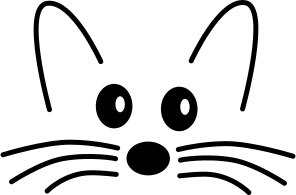
\includegraphics[width=1.4em]{squeak-logo}}}
\newcommand{\dothis}[1]{%
	\medskip
	\noindent\dothisicon
	\ifx#1\empty\else\quad\emph{#1}\fi
	\par\smallskip\nopagebreak}
% NB: To use this in an individual chapter, you must set:
%\graphicspath{{figures/} {../figures/}}
% at the head of the chapter.  Don't forget the final /
%=============================================================
%:Reader hints (hint)
%
% Indicates a non-obvious consequence 
\newcommand{\hint}[1]{\vspace{1ex}\noindent\fbox{\textsc{Astuce}} \emph{#1}}
%=================================================================
% graphics for Morphic handles
\newcommand{\grabHandle}{\raisebox{-0.2ex}{
\includegraphics[width=1em]{blackHandle}}}
\newcommand{\moveHandle}{\raisebox{-0.2ex}{
\includegraphics[width=1em]{moveHandle}}}
\newcommand{\debugHandle}{\raisebox{-0.2ex}{
\includegraphics[width=1em]{debugHandle}}}
% squeak-fr (added for Morphic handles)
\newcommand{\rotateHandle}{\raisebox{-0.2ex}{
\includegraphics[width=1em]{rotateHandle}}}
\newcommand{\viewerHandle}{\raisebox{-0.2ex}{
\includegraphics[width=1em]{viewerHandle}}}
% squeak-fr (add cloverHandle to use \clover in QuickTour.tex as alias
% todo 

%=============================================================
%:Highlighting Important stuff (doublebox)
%
% From Seaside book ...
\newsavebox{\SavedText}
\newlength{\InnerBoxRule}\setlength{\InnerBoxRule}{.75\fboxrule}
\newlength{\OuterBoxRule}\setlength{\OuterBoxRule}{1.5\fboxrule}
\newlength{\BoxSeparation}\setlength{\BoxSeparation}{1.5\fboxrule}
\addtolength{\BoxSeparation}{.5pt}
\newlength{\SaveBoxSep}\setlength{\SaveBoxSep}{2\fboxsep}
%
\newenvironment{doublebox}{\begin{lrbox}{\SavedText}
    \begin{minipage}{.75\textwidth}}
    {\end{minipage}\end{lrbox}\begin{center}
    \setlength{\fboxsep}{\BoxSeparation}\setlength{\fboxrule}{\OuterBoxRule}
    \fbox{\setlength{\fboxsep}{\SaveBoxSep}\setlength{\fboxrule}{\InnerBoxRule}%
      \fbox{\usebox{\SavedText}}}
  \end{center}}
% Use this:
%\newcommand{\important}[1]{\begin{doublebox}#1\end{doublebox}}


\newcommand{\important}[1]{
\noindent\rule{\textwidth}{2pt}\par
\textbf{Important!} #1 \par
\noindent\rule{\textwidth}{2pt}}

\newcommand{\note}[1]{
\noindent\rule{\textwidth}{2pt}\par
\noindent\textbf{Note} #1\par
\noindent\rule{\textwidth}{2pt}}

%=============================================================
%:Section depth
\setcounter{secnumdepth}{2}
%% for this to happen start the file with
%\ifx\wholebook\relax\else
%% $Author$ Martial
% $Date$ Wed Oct 10 13:34:55 CEST 2007
% $Revision$ source: SBE 12715 
% Last Changed Date: 2007-10-08 21:32:45 +0200 (Mon, 08 Oct 2007)
%=============================================================
% NB: documentclass must be set in main document.
% Allows book to be generated in multiple formats.
%=============================================================
%:Packages
%\usepackage[french]{babel}
\usepackage[T1]{fontenc}  %%%%%% really important to get the code directly in the text!
\usepackage{lmodern}
%\usepackage[scaled=0.85]{bookmanx} % needs another scale factor if used with \renewcommand{\sfdefault}{cmbr}
\usepackage{palatino}
%\usepackage[sc]{mathpazo}
%\linespread{1.05}
\usepackage[scaled=0.85]{helvet}
\usepackage{microtype}
\usepackage{graphicx}
\usepackage{theorem}
\usepackage[utf8]{inputenc}
% ON: pdfsync breaks the use of p{width} for tabular columns!
\ifdefined\usepdfsync\usepackage{pdfsync}\fi % Requires texlive 2007
%=============================================================
%:More packages
%Stef should check which ones are used!
%\usepackage{picinpar}
%\usepackage{layout}
%\usepackage{color}
%\definecolor{stefgris}{rgb}{0.85,0.85,0.85}
%\usepackage{enum}
%\usepackage{a4wide}
% \usepackage{fancyhdr}
\usepackage{ifthen}
\usepackage{float}
\usepackage{longtable}
\usepackage{makeidx}
\usepackage[nottoc]{tocbibind}
\usepackage{multicol}
\usepackage{booktabs}	% book-style tables
\usepackage{topcapt}	% enables \topcaption
\usepackage{multirow}
\usepackage{tabularx}
%\usepackage[bottom]{footmisc}
\usepackage{xspace}
\usepackage{alltt}
\usepackage{amssymb,textcomp}
\usepackage[usenames,dvipsnames]{color}
\usepackage{colortbl}
\usepackage[hang]{subfigure}\makeatletter\def\p@subfigure{\thefigure\,}\makeatother
\usepackage{rotating}
\usepackage{enumitem}	% apb: allows more control over tags in enumerations
\usepackage{verbatim}     % for comment environment
\usepackage{varioref}	% for page references that work
\labelformat{footnote}{\thechapter--#1} % to distinguish citations from jurabib
\usepackage{needspace}
\usepackage{isodateo} % enable \isodate
\usepackage[newparttoc]{titlesec}
\usepackage{titletoc}
\usepackage{eurosym}
\usepackage{wrapfig}

\usepackage[
	super,
	citefull=first,
	authorformat={allreversed,and},
	titleformat={commasep,italic}
]{jurabib} % citations as footnotes
\usepackage[
	colorlinks=true,
	linkcolor=black,
	urlcolor=black,
	citecolor=black
]{hyperref}   % should come last

%=============================================================
%:URL style
\makeatletter

\def\url@leostyle{%
  \@ifundefined{selectfont}{\def\UrlFont{\sf}}{\def\UrlFont{\sffamily}}}
% ajouter par Martial pour \traduit (met une dague dans les \doublebox
\def\thempfootnote{\fnsymbol{mpfootnote}}

\makeatother
% Now actually use the newly defined style.
\urlstyle{leo}
%=============================================================
%:Booleans
\newboolean{lulu}
\setboolean{lulu}{false}
\newcommand{\ifluluelse}[2]{\ifthenelse{\boolean{lulu}}{#1}{#2}}
%=============================================================
%:Names
\newcommand{\SUnit}{SUnit\xspace}
\newcommand{\sunit}{SUnit\xspace}
\newcommand{\xUnit}{$x$Unit\xspace}
\newcommand{\JUnit}{JUnit\xspace}
%\newcommand{\XP}{eXtreme Programming\xspace}
\newcommand{\st}{Smalltalk\xspace}
\newcommand{\Squeak}{Squeak\xspace}
\newcommand{\sq}{Squeak\xspace}
\newcommand{\sqmap}{SqueakMap\xspace}
\newcommand{\squeak}{Squeak\xspace}
%\newcommand{\sbe}{\url{scg.unibe.ch/SBE}\xspace}
%\newcommand{\sbe}{\url{squeakbyexample.org}\xspace}
\newcommand{\sbe}{\url{SqueakByExample.org}\xspace}
% squeak-fr: adresse de la version francaise
\newcommand{\spe}{\url{SqueakByExample.org/fr}\xspace}
\newcommand{\sba}{\url{SquareBracketAssociates.org}\xspace}

% squeak-fr: ajout de la \squeakdev pour eviter les problemes de
% changements d'url rencontres dans la VO:
\newcommand{\squeakdev}{\url{www.squeaksource.com/ImageForDevelopers}\xspace} %ou
%\newcommand{\squeakdev}{\url{squeak.ofset.org/squeak-dev}\xspace}

%=============================================================
%:Editorial comment macros
\newcommand{\nnbb}[2]{
    \fbox{\bfseries\sffamily\scriptsize#1}
    {\sf\small$\blacktriangleright$\textit{#2}$\blacktriangleleft$}
   }
\newcommand{\ab}[1]{\nnbb{Andrew}{#1}}
\newcommand{\sd}[1]{\nnbb{St\'{e}f}{#1}}
\newcommand{\md}[1]{\nnbb{Marcus}{#1}}
\newcommand{\on}[1]{\nnbb{Oscar}{#1}}
\newcommand{\damien}[1]{\nnbb{Damien}{#1}}
\newcommand{\lr}[1]{\nnbb{Lukas}{#1}}
\newcommand{\orla}[1]{\nnbb{Orla}{#1}}
%\newcommand{\here}{\nnbb{CONTINUE}{HERE}}
\newcommand{\here}{\nnbb{CONTINUE}{ICI}}

%=============================================================
%:Abbreviation macros
\newcommand{\ie}{\emph{c-\`a-d.}\xspace}
\newcommand{\cad}{\emph{c-\`a-d.}\xspace}
%\newcommand{\eg}{\emph{e.g.},\xspace}
\newcommand{\eg}{\emph{par ex.},\xspace}
\newcommand{\parex}{\emph{par ex.},\xspace}
\newcommand{\etc}{etc\xspace}
%=============================================================
%:Cross reference macros

% [squeak-fr] martial: remarquez les articles devant les noms
\newcommand{\charef}[1]{le chapitre~\ref{cha:#1}\xspace}
% note de martial: utilise dans chapitre Syntax.tex: a redefinir
\newcommand{\charefs}[2]{les chapitres~\ref{cha:#1} et \ref{cha:#2}\xspace}
\newcommand{\secref}[1]{la section~\ref{sec:#1}\xspace}
\newcommand{\figref}[1]{la figure~\ref{fig:#1}\xspace}
\newcommand{\Figref}[1]{La figure~\ref{fig:#1}\xspace}
\newcommand{\appref}[1]{l'annexe~\ref{app:#1}\xspace}
\newcommand{\tabref}[1]{la table~\ref{tab:#1}\xspace}
% defini pour le chapitre Messages.tex
\newcommand{\Tabref}[1]{La table~\ref{tab:#1}\xspace}

% APB: I removed trailing \xspace commands from these macros because
% \xspace mostly doesn't work.  If you want a space after your
% references, type one!
% ON: xspace has always worked just fine for me!  Please leave them in.
%
\newcommand{\ruleref}[1]{\ref{rule:#1}\xspace}
%
\newcommand{\egref}[1]{exemple~\ref{eg:#1}\xspace}
\newcommand{\Egref}[1]{Exemple~\ref{eg:#1}\xspace}
%
\newcommand{\scrref}[1]{script~\ref{scr:#1}\xspace}
\newcommand{\Scrref}[1]{Script~\ref{scr:#1}\xspace}
% t = the
\newcommand{\tscrref}[1]{le script~\ref{scr:#1}\xspace}
\newcommand{\Tscrref}[1]{Le script~\ref{scr:#1}\xspace}
%
\newcommand{\mthref}[1]{m\'ethode~\ref{mth:#1}\xspace}
\newcommand{\mthsref}[1]{m\'ethodes~\ref{mth:#1}\xspace}
\newcommand{\Mthref}[1]{M\'ethode~\ref{mth:#1}\xspace}
\newcommand{\tmthref}[1]{la m\'ethode~\ref{mth:#1}\xspace}
\newcommand{\Tmthref}[1]{La m\'ethode~\ref{mth:#1}\xspace}
%
\newcommand{\clsref}[1]{classe~\ref{cls:#1}\xspace}
\newcommand{\tclsref}[1]{la classe~\ref{cls:#1}\xspace}
\newcommand{\Tclsref}[1]{La classe~\ref{cls:#1}\xspace}
%=============================================================
%:Menu item macro
% for menu items, so we can change our minds on how to print them! (apb)
\definecolor{lightgray}{gray}{0.89}
\newcommand{\menu}[1]{{%
	\setlength{\fboxsep}{0pt}%
	\colorbox{lightgray}{{{\upshape\sffamily\strut \,#1\,}}}}}
% \newcommand{\menu}[1]{{%
% 	\fontfamily{lmr}\selectfont
% 	\upshape\textlangle{\sffamily #1}\textrangle}}
% For submenu items:
\newcommand{\go}{\,$\triangleright$\,}
% \newcommand{\go}{\,$\blacktriangleright$\,}
% For keyboard shortcuts:
%\newcommand{\short}[1]{\mbox{$\langle${\sc CMD}$\rangle$-#1}\xspace}
\newcommand{\short}[1]{\mbox{{\sc cmd}\hspace{0.08em}--\hspace{0.09em}#1}\xspace}
% For buttons:
\newcommand{\button}[1]{{%
	\setlength{\fboxsep}{0pt}%
	\fbox{{\upshape\sffamily\strut \,#1\,}}}}
\newcommand{\toolsflap}{l'onglet \textit{Tools}\xspace}
%=============================================================
%:Reader cues (do this)
%
% Indicate something the reader should try out.
\newcommand{\dothisicon}{\raisebox{-.5ex}{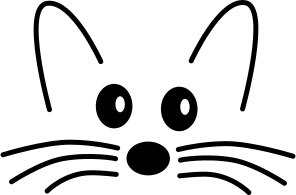
\includegraphics[width=1.4em]{squeak-logo}}}
\newcommand{\dothis}[1]{%
	\medskip
	\noindent\dothisicon
	\ifx#1\empty\else\quad\emph{#1}\fi
	\par\smallskip\nopagebreak}
% NB: To use this in an individual chapter, you must set:
%\graphicspath{{figures/} {../figures/}}
% at the head of the chapter.  Don't forget the final /
%=============================================================
%:Reader hints (hint)
%
% Indicates a non-obvious consequence 
\newcommand{\hint}[1]{\vspace{1ex}\noindent\fbox{\textsc{Astuce}} \emph{#1}}
%=================================================================
% graphics for Morphic handles
\newcommand{\grabHandle}{\raisebox{-0.2ex}{
\includegraphics[width=1em]{blackHandle}}}
\newcommand{\moveHandle}{\raisebox{-0.2ex}{
\includegraphics[width=1em]{moveHandle}}}
\newcommand{\debugHandle}{\raisebox{-0.2ex}{
\includegraphics[width=1em]{debugHandle}}}
% squeak-fr (added for Morphic handles)
\newcommand{\rotateHandle}{\raisebox{-0.2ex}{
\includegraphics[width=1em]{rotateHandle}}}
\newcommand{\viewerHandle}{\raisebox{-0.2ex}{
\includegraphics[width=1em]{viewerHandle}}}
% squeak-fr (add cloverHandle to use \clover in QuickTour.tex as alias
% todo 

%=============================================================
%:Highlighting Important stuff (doublebox)
%
% From Seaside book ...
\newsavebox{\SavedText}
\newlength{\InnerBoxRule}\setlength{\InnerBoxRule}{.75\fboxrule}
\newlength{\OuterBoxRule}\setlength{\OuterBoxRule}{1.5\fboxrule}
\newlength{\BoxSeparation}\setlength{\BoxSeparation}{1.5\fboxrule}
\addtolength{\BoxSeparation}{.5pt}
\newlength{\SaveBoxSep}\setlength{\SaveBoxSep}{2\fboxsep}
%
\newenvironment{doublebox}{\begin{lrbox}{\SavedText}
    \begin{minipage}{.75\textwidth}}
    {\end{minipage}\end{lrbox}\begin{center}
    \setlength{\fboxsep}{\BoxSeparation}\setlength{\fboxrule}{\OuterBoxRule}
    \fbox{\setlength{\fboxsep}{\SaveBoxSep}\setlength{\fboxrule}{\InnerBoxRule}%
      \fbox{\usebox{\SavedText}}}
  \end{center}}
% Use this:
%\newcommand{\important}[1]{\begin{doublebox}#1\end{doublebox}}


\newcommand{\important}[1]{
\noindent\rule{\textwidth}{2pt}\par
\textbf{Important!} #1 \par
\noindent\rule{\textwidth}{2pt}}

\newcommand{\note}[1]{
\noindent\rule{\textwidth}{2pt}\par
\noindent\textbf{Note} #1\par
\noindent\rule{\textwidth}{2pt}}

%=============================================================
%:Section depth
\setcounter{secnumdepth}{2}
%% for this to happen start the file with
%\ifx\wholebook\relax\else
%% $Author$ Martial
% $Date$ Wed Oct 10 13:34:55 CEST 2007
% $Revision$ source: SBE 12715 
% Last Changed Date: 2007-10-08 21:32:45 +0200 (Mon, 08 Oct 2007)
%=============================================================
% NB: documentclass must be set in main document.
% Allows book to be generated in multiple formats.
%=============================================================
%:Packages
%\usepackage[french]{babel}
\usepackage[T1]{fontenc}  %%%%%% really important to get the code directly in the text!
\usepackage{lmodern}
%\usepackage[scaled=0.85]{bookmanx} % needs another scale factor if used with \renewcommand{\sfdefault}{cmbr}
\usepackage{palatino}
%\usepackage[sc]{mathpazo}
%\linespread{1.05}
\usepackage[scaled=0.85]{helvet}
\usepackage{microtype}
\usepackage{graphicx}
\usepackage{theorem}
\usepackage[utf8]{inputenc}
% ON: pdfsync breaks the use of p{width} for tabular columns!
\ifdefined\usepdfsync\usepackage{pdfsync}\fi % Requires texlive 2007
%=============================================================
%:More packages
%Stef should check which ones are used!
%\usepackage{picinpar}
%\usepackage{layout}
%\usepackage{color}
%\definecolor{stefgris}{rgb}{0.85,0.85,0.85}
%\usepackage{enum}
%\usepackage{a4wide}
% \usepackage{fancyhdr}
\usepackage{ifthen}
\usepackage{float}
\usepackage{longtable}
\usepackage{makeidx}
\usepackage[nottoc]{tocbibind}
\usepackage{multicol}
\usepackage{booktabs}	% book-style tables
\usepackage{topcapt}	% enables \topcaption
\usepackage{multirow}
\usepackage{tabularx}
%\usepackage[bottom]{footmisc}
\usepackage{xspace}
\usepackage{alltt}
\usepackage{amssymb,textcomp}
\usepackage[usenames,dvipsnames]{color}
\usepackage{colortbl}
\usepackage[hang]{subfigure}\makeatletter\def\p@subfigure{\thefigure\,}\makeatother
\usepackage{rotating}
\usepackage{enumitem}	% apb: allows more control over tags in enumerations
\usepackage{verbatim}     % for comment environment
\usepackage{varioref}	% for page references that work
\labelformat{footnote}{\thechapter--#1} % to distinguish citations from jurabib
\usepackage{needspace}
\usepackage{isodateo} % enable \isodate
\usepackage[newparttoc]{titlesec}
\usepackage{titletoc}
\usepackage{eurosym}
\usepackage{wrapfig}

\usepackage[
	super,
	citefull=first,
	authorformat={allreversed,and},
	titleformat={commasep,italic}
]{jurabib} % citations as footnotes
\usepackage[
	colorlinks=true,
	linkcolor=black,
	urlcolor=black,
	citecolor=black
]{hyperref}   % should come last

%=============================================================
%:URL style
\makeatletter

\def\url@leostyle{%
  \@ifundefined{selectfont}{\def\UrlFont{\sf}}{\def\UrlFont{\sffamily}}}
% ajouter par Martial pour \traduit (met une dague dans les \doublebox
\def\thempfootnote{\fnsymbol{mpfootnote}}

\makeatother
% Now actually use the newly defined style.
\urlstyle{leo}
%=============================================================
%:Booleans
\newboolean{lulu}
\setboolean{lulu}{false}
\newcommand{\ifluluelse}[2]{\ifthenelse{\boolean{lulu}}{#1}{#2}}
%=============================================================
%:Names
\newcommand{\SUnit}{SUnit\xspace}
\newcommand{\sunit}{SUnit\xspace}
\newcommand{\xUnit}{$x$Unit\xspace}
\newcommand{\JUnit}{JUnit\xspace}
%\newcommand{\XP}{eXtreme Programming\xspace}
\newcommand{\st}{Smalltalk\xspace}
\newcommand{\Squeak}{Squeak\xspace}
\newcommand{\sq}{Squeak\xspace}
\newcommand{\sqmap}{SqueakMap\xspace}
\newcommand{\squeak}{Squeak\xspace}
%\newcommand{\sbe}{\url{scg.unibe.ch/SBE}\xspace}
%\newcommand{\sbe}{\url{squeakbyexample.org}\xspace}
\newcommand{\sbe}{\url{SqueakByExample.org}\xspace}
% squeak-fr: adresse de la version francaise
\newcommand{\spe}{\url{SqueakByExample.org/fr}\xspace}
\newcommand{\sba}{\url{SquareBracketAssociates.org}\xspace}

% squeak-fr: ajout de la \squeakdev pour eviter les problemes de
% changements d'url rencontres dans la VO:
\newcommand{\squeakdev}{\url{www.squeaksource.com/ImageForDevelopers}\xspace} %ou
%\newcommand{\squeakdev}{\url{squeak.ofset.org/squeak-dev}\xspace}

%=============================================================
%:Editorial comment macros
\newcommand{\nnbb}[2]{
    \fbox{\bfseries\sffamily\scriptsize#1}
    {\sf\small$\blacktriangleright$\textit{#2}$\blacktriangleleft$}
   }
\newcommand{\ab}[1]{\nnbb{Andrew}{#1}}
\newcommand{\sd}[1]{\nnbb{St\'{e}f}{#1}}
\newcommand{\md}[1]{\nnbb{Marcus}{#1}}
\newcommand{\on}[1]{\nnbb{Oscar}{#1}}
\newcommand{\damien}[1]{\nnbb{Damien}{#1}}
\newcommand{\lr}[1]{\nnbb{Lukas}{#1}}
\newcommand{\orla}[1]{\nnbb{Orla}{#1}}
%\newcommand{\here}{\nnbb{CONTINUE}{HERE}}
\newcommand{\here}{\nnbb{CONTINUE}{ICI}}

%=============================================================
%:Abbreviation macros
\newcommand{\ie}{\emph{c-\`a-d.}\xspace}
\newcommand{\cad}{\emph{c-\`a-d.}\xspace}
%\newcommand{\eg}{\emph{e.g.},\xspace}
\newcommand{\eg}{\emph{par ex.},\xspace}
\newcommand{\parex}{\emph{par ex.},\xspace}
\newcommand{\etc}{etc\xspace}
%=============================================================
%:Cross reference macros

% [squeak-fr] martial: remarquez les articles devant les noms
\newcommand{\charef}[1]{le chapitre~\ref{cha:#1}\xspace}
% note de martial: utilise dans chapitre Syntax.tex: a redefinir
\newcommand{\charefs}[2]{les chapitres~\ref{cha:#1} et \ref{cha:#2}\xspace}
\newcommand{\secref}[1]{la section~\ref{sec:#1}\xspace}
\newcommand{\figref}[1]{la figure~\ref{fig:#1}\xspace}
\newcommand{\Figref}[1]{La figure~\ref{fig:#1}\xspace}
\newcommand{\appref}[1]{l'annexe~\ref{app:#1}\xspace}
\newcommand{\tabref}[1]{la table~\ref{tab:#1}\xspace}
% defini pour le chapitre Messages.tex
\newcommand{\Tabref}[1]{La table~\ref{tab:#1}\xspace}

% APB: I removed trailing \xspace commands from these macros because
% \xspace mostly doesn't work.  If you want a space after your
% references, type one!
% ON: xspace has always worked just fine for me!  Please leave them in.
%
\newcommand{\ruleref}[1]{\ref{rule:#1}\xspace}
%
\newcommand{\egref}[1]{exemple~\ref{eg:#1}\xspace}
\newcommand{\Egref}[1]{Exemple~\ref{eg:#1}\xspace}
%
\newcommand{\scrref}[1]{script~\ref{scr:#1}\xspace}
\newcommand{\Scrref}[1]{Script~\ref{scr:#1}\xspace}
% t = the
\newcommand{\tscrref}[1]{le script~\ref{scr:#1}\xspace}
\newcommand{\Tscrref}[1]{Le script~\ref{scr:#1}\xspace}
%
\newcommand{\mthref}[1]{m\'ethode~\ref{mth:#1}\xspace}
\newcommand{\mthsref}[1]{m\'ethodes~\ref{mth:#1}\xspace}
\newcommand{\Mthref}[1]{M\'ethode~\ref{mth:#1}\xspace}
\newcommand{\tmthref}[1]{la m\'ethode~\ref{mth:#1}\xspace}
\newcommand{\Tmthref}[1]{La m\'ethode~\ref{mth:#1}\xspace}
%
\newcommand{\clsref}[1]{classe~\ref{cls:#1}\xspace}
\newcommand{\tclsref}[1]{la classe~\ref{cls:#1}\xspace}
\newcommand{\Tclsref}[1]{La classe~\ref{cls:#1}\xspace}
%=============================================================
%:Menu item macro
% for menu items, so we can change our minds on how to print them! (apb)
\definecolor{lightgray}{gray}{0.89}
\newcommand{\menu}[1]{{%
	\setlength{\fboxsep}{0pt}%
	\colorbox{lightgray}{{{\upshape\sffamily\strut \,#1\,}}}}}
% \newcommand{\menu}[1]{{%
% 	\fontfamily{lmr}\selectfont
% 	\upshape\textlangle{\sffamily #1}\textrangle}}
% For submenu items:
\newcommand{\go}{\,$\triangleright$\,}
% \newcommand{\go}{\,$\blacktriangleright$\,}
% For keyboard shortcuts:
%\newcommand{\short}[1]{\mbox{$\langle${\sc CMD}$\rangle$-#1}\xspace}
\newcommand{\short}[1]{\mbox{{\sc cmd}\hspace{0.08em}--\hspace{0.09em}#1}\xspace}
% For buttons:
\newcommand{\button}[1]{{%
	\setlength{\fboxsep}{0pt}%
	\fbox{{\upshape\sffamily\strut \,#1\,}}}}
\newcommand{\toolsflap}{l'onglet \textit{Tools}\xspace}
%=============================================================
%:Reader cues (do this)
%
% Indicate something the reader should try out.
\newcommand{\dothisicon}{\raisebox{-.5ex}{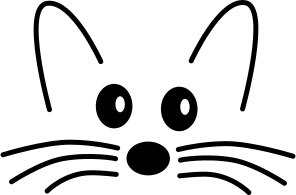
\includegraphics[width=1.4em]{squeak-logo}}}
\newcommand{\dothis}[1]{%
	\medskip
	\noindent\dothisicon
	\ifx#1\empty\else\quad\emph{#1}\fi
	\par\smallskip\nopagebreak}
% NB: To use this in an individual chapter, you must set:
%\graphicspath{{figures/} {../figures/}}
% at the head of the chapter.  Don't forget the final /
%=============================================================
%:Reader hints (hint)
%
% Indicates a non-obvious consequence 
\newcommand{\hint}[1]{\vspace{1ex}\noindent\fbox{\textsc{Astuce}} \emph{#1}}
%=================================================================
% graphics for Morphic handles
\newcommand{\grabHandle}{\raisebox{-0.2ex}{
\includegraphics[width=1em]{blackHandle}}}
\newcommand{\moveHandle}{\raisebox{-0.2ex}{
\includegraphics[width=1em]{moveHandle}}}
\newcommand{\debugHandle}{\raisebox{-0.2ex}{
\includegraphics[width=1em]{debugHandle}}}
% squeak-fr (added for Morphic handles)
\newcommand{\rotateHandle}{\raisebox{-0.2ex}{
\includegraphics[width=1em]{rotateHandle}}}
\newcommand{\viewerHandle}{\raisebox{-0.2ex}{
\includegraphics[width=1em]{viewerHandle}}}
% squeak-fr (add cloverHandle to use \clover in QuickTour.tex as alias
% todo 

%=============================================================
%:Highlighting Important stuff (doublebox)
%
% From Seaside book ...
\newsavebox{\SavedText}
\newlength{\InnerBoxRule}\setlength{\InnerBoxRule}{.75\fboxrule}
\newlength{\OuterBoxRule}\setlength{\OuterBoxRule}{1.5\fboxrule}
\newlength{\BoxSeparation}\setlength{\BoxSeparation}{1.5\fboxrule}
\addtolength{\BoxSeparation}{.5pt}
\newlength{\SaveBoxSep}\setlength{\SaveBoxSep}{2\fboxsep}
%
\newenvironment{doublebox}{\begin{lrbox}{\SavedText}
    \begin{minipage}{.75\textwidth}}
    {\end{minipage}\end{lrbox}\begin{center}
    \setlength{\fboxsep}{\BoxSeparation}\setlength{\fboxrule}{\OuterBoxRule}
    \fbox{\setlength{\fboxsep}{\SaveBoxSep}\setlength{\fboxrule}{\InnerBoxRule}%
      \fbox{\usebox{\SavedText}}}
  \end{center}}
% Use this:
%\newcommand{\important}[1]{\begin{doublebox}#1\end{doublebox}}


\newcommand{\important}[1]{
\noindent\rule{\textwidth}{2pt}\par
\textbf{Important!} #1 \par
\noindent\rule{\textwidth}{2pt}}

\newcommand{\note}[1]{
\noindent\rule{\textwidth}{2pt}\par
\noindent\textbf{Note} #1\par
\noindent\rule{\textwidth}{2pt}}

%=============================================================
%:Section depth
\setcounter{secnumdepth}{2}
%% for this to happen start the file with
%\ifx\wholebook\relax\else
%\input{../common.tex}
%\begin{document}
%\fi
% and terminate by
% \ifx\wholebook\relax\else\end{document}\fi

\DeclareGraphicsExtensions{.pdf, .jpg, .png}
%=============================================================
%:PDF setup
\hypersetup{
%   a4paper,
%   pdfstartview=FitV,
%   colorlinks,
%   linkcolor=darkblue,
%   citecolor=darkblue,
%   pdftitle={Squeak by Example},
pdftitle={Squeak par l'exemple},
   pdfauthor={Andrew Black, St\'ephane Ducasse,	Oscar Nierstrasz,
Damien Pollet},
   pdfkeywords={Smalltalk, Squeak, Programmation Orient\'ee Objet},
pdfsubject={Informatique, Computer Science}
}
%=============================================================
%:Page layout and appearance
%
% \renewcommand{\headrulewidth}{0pt}
\renewcommand{\chaptermark}[1]{\markboth{#1}{}}
\renewcommand{\sectionmark}[1]{\markright{\thesection\ #1}}
\renewpagestyle{plain}[\small\itshape]{%
	\setheadrule{0pt}%
	\sethead[][][]{}{}{}%
	\setfoot[][][]{}{}{}}
\renewpagestyle{headings}[\small\itshape]{%
	\setheadrule{0pt}%
	\setmarks{chapter}{section}%
	\sethead[\thepage][][\chaptertitle]{\sectiontitle}{}{\thepage}%
	\setfoot[][][]{}{}{}}
% pagestyle for tableofcontents + index (martial: 2008/04/23)
\newpagestyle{newheadings}[\small\itshape]{%
	\setheadrule{0pt}%
	\setmarks{chapter}{section}%
	\sethead[\thepage][][\chaptertitle]{\chaptertitle}{}{\thepage}%
	\setfoot[][][]{}{}{}}
%=============================================================
%:Title section setup and TOC numbering depth
\setcounter{secnumdepth}{1}
\setcounter{tocdepth}{1}
\titleformat{\part}[display]{\centering}{\huge\partname\ \thepart}{1em}{\Huge\textbf}[]
\titleformat{\chapter}[display]{}{\huge\chaptertitlename\ \thechapter}{1em}{\Huge\raggedright\textbf}[]
\titlecontents{part}[3pc]{%
		\pagebreak[2]\addvspace{1em plus.4em minus.2em}%
		\leavevmode\large\bfseries}
	{\contentslabel{3pc}}{\hspace*{-3pc}}
	{}[\nopagebreak]
\titlecontents{chapter}[3pc]{%
		\pagebreak[0]\addvspace{1em plus.2em minus.2em}%
		\leavevmode\bfseries}
	{\contentslabel{3pc}}{}
	{\hfill\contentspage}[\nopagebreak]
\dottedcontents{section}[3pc]{}{3pc}{1pc}
\dottedcontents{subsection}[3pc]{}{0pc}{1pc}
% \dottedcontents{subsection}[4.5em]{}{0pt}{1pc}
% Make \cleardoublepage insert really blank pages http://www.tex.ac.uk/cgi-bin/texfaq2html?label=reallyblank
\let\origdoublepage\cleardoublepage
\newcommand{\clearemptydoublepage}{%
  \clearpage
  {\pagestyle{empty}\origdoublepage}}
\let\cleardoublepage\clearemptydoublepage % see http://www.tex.ac.uk/cgi-bin/texfaq2html?label=patch
%=============================================================
%:FAQ macros (for FAQ chapter)
\newtheorem{faq}{FAQ}
\newcommand{\answer}{\paragraph{R\'eponse}\ }
%=============================================================
%:Listings package configuration
\usepackage{listings}
\newcommand{\caret}{\makebox{\raisebox{0.4ex}{\footnotesize{$\wedge$}}}}
\lstdefinelanguage{Smalltalk}{
%  morekeywords={self,super,true,false,nil,thisContext}, % This is overkill
  morestring=[d]',
  morecomment=[s]{"}{"},
  alsoletter={\#:},
  escapechar={!},
  escapebegin=\itshape, % comment-like by default (Martial 11/2007)
  literate=
    {BANG}{!}1
    {UNDERSCORE}{\_}1
    {\\st}{Smalltalk}9 % convenience -- in case \st occurs in code
    % {'}{{\textquotesingle}}1 % replaced by upquote=true in \lstset
    {_}{{$\leftarrow$}}1
    {>>>}{{\sep}}1
    {^}{{$\uparrow$}}1
    {~}{{$\sim$}}1
    {-}{{\sf -\hspace{-0.13em}-}}1  % the goal is to make - the same width as +
    {+}{\raisebox{0.08ex}{+}}1		% and to raise + off the baseline to match -
    {-->}{{\quad$\longrightarrow$\quad}}3
	, % Don't forget the comma at the end!
  tabsize=4
}[keywords,comments,strings]
% ajout pour les échappements dans les codes
% indispensable pour mettre le code en emphase (cf. Model.tex) 
\newcommand{\codeify}[1]{\NoAutoSpaceBeforeFDP#1\AutoSpaceBeforeFDP}
\newcommand{\normcomment}[1]{\emph{#1}} %cf. Streams
\newcommand{\normcode}[1]{\emph{\codeify{#1}}} %cf. Streams
\newcommand{\emcode}[1]{\textbf{\normcode{#1}}} % Martial 11/2007
\lstset{language=Smalltalk,
	basicstyle=\sffamily,
	keywordstyle=\color{black}\bfseries,
	% stringstyle=\ttfamily, % Ugly! do we really want this? -- on
	%commentstyle=\itshape,
	mathescape=true,
	showstringspaces=false,
	keepspaces=true,
	breaklines=true,
	breakautoindent=true,
	lineskip={-1pt}, % Ugly hack
	upquote=true, % straight quote; requires textcomp package
	columns=fullflexible} % no fixed width fonts
% In-line code (literal)
% Normally use this for all in-line code:
\newcommand{\ct}{\lstinline[mathescape=false,basicstyle={\sffamily\upshape}]}
% apb 2007.8.28 added the \upshape declaration to avoid getting italicized code in \dothis{ } sections.
% In-line code (latex enabled)
% Use this only in special situations where \ct does not work
% (within section headings ...):

% [squeak-fr] Modification de \lct suivant les indications de Martial Boniou
\newcommand{\lct}[1]{\textsf{\textup{\NoAutoSpaceBeforeFDP #1
\AutoSpaceBeforeFDP}}} %\xspace

% Use these for system categories and protocols:
\newcommand{\scat}[1]{\emph{\textsf{#1}}\xspace}
\newcommand{\pkg}[1]{\emph{\textsf{#1}}\xspace}
\newcommand{\prot}[1]{\emph{\textsf{#1}}\xspace}
% Code environments
% NB: the arg is for tests
% Only code and example environments may be tests
\lstnewenvironment{code}[1]{%
	\lstset{%
		frame=lines,
		mathescape=false
	}
}{}
\def\ignoredollar#1{}
%=============================================================
%:Code environments (method, script ...)
% NB: the third arg is for tests
% Only code and example environments may be tests
\lstnewenvironment{example}[3][defaultlabel]{%
	\renewcommand{\lstlistingname}{Exemple}%
	\lstset{
		frame=lines,
		mathescape=false,
		caption={\emph{#2}},
		label={eg:#1}
	}
}{}
\lstnewenvironment{script}[2][defaultlabel]{%
\renewcommand{\lstlistingname}{Script}%
	\lstset{
		frame=lines,
		mathescape=false,
		name={Script},
		caption={\emph{#2}},
		label={scr:#1}
	}
}{}
%I could not find a way yo get the Experiment #numb followed by the caption in a black box
%\colorbox{black}{\makebox[\textwidth]{  \color{white} {\large {\bfseries Experiment 3-1 (crear i moure un robot)}} }}
\lstnewenvironment{experiment}[2][defaultlabel]{%
%\noindent\rule{\textwidth}{2pt}\vspace{-0.8cm}
\renewcommand{\lstlistingname}{Experiment}%
	\lstset{
		frame=none,
		rulecolor=\color{black},
		mathescape=false,
		name={Experiment},
		caption={\emph{#2}},
		label={scr:#1}
	}
}{%\vspace{-0.5cm}\noindent\rule{\textwidth}{2pt}
}

\lstnewenvironment{method}[2][defaultlabel]{%
	\renewcommand{\lstlistingname}{Method}%
	\lstset{
		frame=lines,
		mathescape=false,
		name={M\'ethode},
		caption={\emph{#2}},
		label={mth:#1}
	}
}{}
\lstnewenvironment{methods}[2][defaultlabel]{% just for multiple methods at once
	\renewcommand{\lstlistingname}{Methods}%
	\lstset{
		frame=lines,
		mathescape=false,
		name={M\'ethode},
		caption={\emph{#2}},
		label={mth:#1}
	}
}{}
\lstnewenvironment{numMethod}[2][defaultlabel]{%
	\renewcommand{\lstlistingname}{Method}%
	\lstset{
		numbers=left,
		numberstyle={\tiny\sffamily},
		frame=lines,
		mathescape=false,
		name={M\'ethode},
		caption={\emph{#2}},
		label={mth:#1}
	}
}{}
% \lstnewenvironment{classdef}[2][defaultlabel]{%
% 	\renewcommand{\lstlistingname}{Classe}%
% 	\lstset{
% 		frame=lines,
% 		mathescape=false,
% 		name={Classe},
% 		caption={\emph{#2}},
% 		label={cls:#1}
% 	}
% }{}

%%%%%%%%%%%%%%%%%%%%%%%%%%%%%%%%%%%%%%%%%%%%%%%%%%%%%%%%%%%%%%%%%%%%%%%%%%%%%%%%%%%%%%%%%%%%%%%%%
%%From the original book latex template
%%%%%%%%%%%%%%%%%%%%%%%%%%%%%%%%%%%%%%%%%%%%%%%%%%%%%%%%%%%%%%%%%%%%%%%%%%%%%%%%%%%%%%%%%%%%%%%%%
\theoremstyle{break}
{\theorembodyfont{\rmfamily}\theoremstyle{break}
\newtheorem{privScript}{Script}[chapter]
%\newtheorem{privMethod}{Method}[chapter]
\newtheorem{privExercise}{Experiment}[chapter]}

% \theoremstyle{break}
% {\theorembodyfont{\rmfamily} \newtheorem{privMethod}{Method}[chapter]}

%class
\theoremstyle{break}
{\theorembodyfont{\rmfamily} \newtheorem{privClassDef}{Class}[chapter]}

%important
\theoremstyle{break}
{\theorembodyfont{\rmfamily} \newtheorem{privTemplate}{Important Messages}[chapter]}

% experiment
\newenvironment{exercise}
    {\begin{privExercise}\mbox{}\\}
    {\end{privExercise}}


%%% for figure
\newsavebox{\ScriptFigure}
\newlength{\ScriptWidth}
\newlength{\FigureWidth}

%%%%%%%%%%%%%%%%%%%%%%%%%%%%%%%%%%%%%%%%%%%%%%%%%%%%%%%%%%%%%%%%%%%%%%%%%%%%%%%%
\newenvironment{scriptfig}[3][0.6]
   {\setlength{\ScriptWidth}{\linewidth*\real{#1}}%
   \setlength{\FigureWidth}{\linewidth-(\linewidth*\real{#1})}%
   \savebox{\ScriptFigure}%
	{\parbox{\FigureWidth}{\includegraphics[width=0.98\FigureWidth]{#2}}}%
   \par\noindent\begin{minipage}{\linewidth}\hrule\vskip 0.2cm\begin{minipage}[c]{\ScriptWidth}%
   \begin{stefscript}[{\em #3}]\begin{alltt}\sffamily}
   {\end{alltt}\end{stefscript}\end{minipage}\hfill
   \usebox{\ScriptFigure}
   \vskip 1ex\hrule\end{minipage}\vskip 1ex\par}

%%%%%%%%%%%%%%%%%%%%%%%%%%%%%%%%%%%%%%%%%%%%%%%%%%%%%%%%%%%%%%%%%%%%%%%%%%%%%%%%
%% to be able to specify the complete set of values for includegraphics
%% may be will be changed but not the interface
\newenvironment{scriptfigwithsize}[3][0.6]
   {\setlength{\ScriptWidth}{\linewidth*\real{#1}}%
   \setlength{\FigureWidth}{\linewidth-(\linewidth*\real{#1})}%
   \savebox{\ScriptFigure}{\parbox{\FigureWidth}{\raggedleft{#2}}}%
   \par\noindent\begin{minipage}{\linewidth}\hrule\vskip 0.3cm\begin{minipage}[c]{\ScriptWidth}%
   \begin{stefscript}[{\em #3}]\begin{alltt}\sffamily}
   {\end{alltt}\end{stefscript}\end{minipage}\hfill
   \usebox{\ScriptFigure}
   \vskip 1ex\hrule\end{minipage}\vskip 1ex\par}

% \newenvironment{methodfig}[2][0.6]
%    {\setlength{\ScriptWidth}{\linewidth*\real{#1}}%
%    \setlength{\FigureWidth}{\linewidth-(\linewidth*\real{#1})}%
%    \savebox{\ScriptFigure}{\parbox{\FigureWidth}{\includegraphics[width=.98\FigureWidth]{#2}}}%
%    \par\noindent\rule{\linewidth}{1mm}
%    \\[-0.3cm]\noindent\rule{\linewidth}{0.1mm}
%    \noindent\begin{minipage}[c]{\ScriptWidth}\begin{privMethod}\begin{alltt}\sffamily}
%    {\end{alltt}\end{privMethod}\end{minipage}\hfill
%    \usebox{\ScriptFigure} \vskip 1ex\hrule\vskip 1ex\par}

% \newenvironment{method}
% {\par\noindent\begin{minipage}{\linewidth}\vspace{0.2cm}\begin{privMethod}\begin{nminipage}\vspace{-0.2cm}\rule{\linewidth}{1mm}\\[-0.6cm]\rule{\linewidth}{0.1mm}\end{nminipage}\hspace*{\scriptindent}\codesize\begin{nalltt}\vspace{-0.2cm}}
% {\end{nalltt}\normalsize\vspace{-0.1cm}\hrule\end{privMethod}\vspace{0.2cm}\end{minipage}}


% \newenvironment{classdef}
% {\par\noindent\begin{minipage}{\linewidth}\vspace{0.2cm}\begin{privClassDef}\begin{nminipage}\vspace{-0.2cm}\rule{\linewidth}{1mm}\\[-0.6cm]\rule{\linewidth}{0.1mm}\end{nminipage}\hspace*{\scriptindent}\codesize\begin{nalltt}\vspace{-0.2cm}}
% {\end{nalltt}\normalsize\vspace{-0.1cm}\hrule\end{privClassDef}\vspace{0.2cm}\end{minipage}}


% \newenvironment{template}
% {\par\noindent\begin{minipage}{\linewidth}\vspace{0.3cm}\begin{privTemplate}\begin{nminipage}\vspace{-0.4cm}\rule{\linewidth}{0.1mm}\end{nminipage}\hspace*{\scriptindent}\begin{nalltt}\vspace{-0.7cm}}
% {\end{nalltt}\vspace{-0.1cm}\hrule\end{privTemplate}\end{minipage}\vspace{0.3cm}}

\newenvironment{exofig}[2][0.7]
   {\setlength{\ScriptWidth}{\linewidth*\real{#1}}
   \setlength{\FigureWidth}{\linewidth-(\linewidth*\real{#1})}
   \savebox{\ScriptFigure}{\parbox{\FigureWidth}{\raggedleft{\includegraphics[width=.98\FigureWidth]{#2}}}}
   \par\noindent\begin{minipage}{\linewidth}\hrule\vskip 0.3cm\begin{minipage}[c]{\ScriptWidth}%
   \begin{privExercise}}
   {\end{privExercise}\end{minipage}\hfill
   \usebox{\ScriptFigure}
   \vskip 1ex\hrule\end{minipage}\vskip 1ex\par}

\newenvironment{exofigwithsize}[2][0.7]
   {\setlength{\ScriptWidth}{\linewidth*\real{#1}}
   \setlength{\FigureWidth}{\linewidth-(\linewidth*\real{#1})}
   \savebox{\ScriptFigure}{\parbox{\FigureWidth}{\raggedleft{#2}}}
   \par\noindent\begin{minipage}{\linewidth}\hrule\vskip 0.3cm\begin{minipage}[c]{\ScriptWidth}%
   \begin{privExercise}}
   {\end{privExercise}\end{minipage}\hfill\usebox{\ScriptFigure}
   \vskip 1ex\hrule\end{minipage}\vskip 1ex\par}

\newenvironment{exofigwithsizeandtitle}[3][0.7]
   {\setlength{\ScriptWidth}{\linewidth*\real{#1}}
   \setlength{\FigureWidth}{\linewidth-(\linewidth*\real{#1})}
   \savebox{\ScriptFigure}{\parbox{\FigureWidth}{\raggedleft{#2}}}
   \vskip 0.3cm\par\noindent\begin{minipage}{\linewidth}\hrule\vskip 0.1cm\begin{minipage}[c]{\ScriptWidth}%
   \begin{privExercise}[\em{#3}]}
   {\end{privExercise}\end{minipage}\hfill\usebox{\ScriptFigure}
   \vskip 1ex\hrule\end{minipage}\vskip 1ex\par}

\newenvironment{exofigwithtitle}[3][0.7]
   {\setlength{\ScriptWidth}{\linewidth*\real{#1}}
   \setlength{\FigureWidth}{\linewidth-(\linewidth*\real{#1})}
   \savebox{\ScriptFigure}{\parbox{\FigureWidth}{\raggedleft{\includegraphics[width=.98\FigureWidth]{#2}}}}
   \par\noindent\begin{minipage}{\linewidth}\hrule\vskip 0.3cm\begin{minipage}[c]{\ScriptWidth}%
   \begin{privExercise}[\em{#3}]}
   {\end{privExercise}\end{minipage}\hfill
   \usebox{\ScriptFigure}
   \vskip 1ex\hrule\end{minipage}\vskip 1ex\par}


\newenvironment{exonofigwithtitle}[3][0.7]
   {\setlength{\ScriptWidth}{\linewidth*\real{#1}}
   \setlength{\FigureWidth}{\linewidth-(\linewidth*\real{#1})}
   \savebox{\ScriptFigure}{\parbox{\FigureWidth}{\raggedleft{\includegraphics[width=.98\FigureWidth]{#2}}}}
   \par\noindent\begin{minipage}{\linewidth}\hrule\vskip 0.3cm\begin{minipage}[c]{\ScriptWidth}%
   \begin{privExercise}[\em{#3}]}
   {\end{privExercise}\end{minipage}\hfill
   \usebox{\ScriptFigure}
   \vskip 1ex\hrule\end{minipage}\vskip 1ex\par}

\newenvironment{exonofig}
   {\par\noindent\begin{minipage}[t]{\linewidth}\noindent\begin{privExercise}}
   {\end{privExercise}\end{minipage}\vspace{0.5cm}\par}

\newenvironment{exonofigtitle}[1]
   {\par\noindent\begin{minipage}[t]{\linewidth}\noindent\begin{privExercise}[\em{#1}]}
   {\end{privExercise}\end{minipage}\vspace{0.5cm}\par}
		
% \newenvironment{solfig}[3][0.5]
%    {\setlength{\ScriptWidth}{\linewidth*\real{#1}}
%    \setlength{\FigureWidth}{\linewidth-\linewidth*\real{#1}}
%    \savebox{\ScriptFigure}{\parbox{\FigureWidth}{\includegraphics[width=.9\linewidth]{#2}}}
%    \par\noindent\vskip 1ex\hrule\vskip 1ex\begin{minipage}[t]{\ScriptWidth}
%    {\bf Solution #3} \begin{alltt}\sffamily}
%    {\end{alltt}\end{minipage}\hfill
%    \usebox{\ScriptFigure}
%    \vskip 1ex\hrule\vskip 1ex\par}
% 
% \newenvironment{solnofig}[1]
%    {\par\noindent\vskip 1ex\hrule\vskip 1ex\begin{minipage}[t]{\ScriptWidth}
%    {\bf Solution #1} \begin{alltt}\sffamily}
%    {\end{alltt}\end{minipage}\hfill
%    \vskip 1ex\hrule\vskip 1ex\par}
% 
% \newenvironment{exoscript}[3][0.5]
%    {\setlength{\ScriptWidth}{\linewidth*\real{#1}}
%     \setlength{\FigureWidth}{\linewidth-\linewidth*\real{#1}}
%     \savebox{\ScriptFigure}{\begin{minipage}\begin{alltt}\sffamily#3\end{alltt}\end{minipage}}
%     \par\noindent\vskip 1ex\hrule\vskip 1ex\begin{minipage}[t]{\ScriptWidth}
%     \begin{privExercise}}
%     {\end{privExercise}\end{minipage}\hfill
%     \usebox{\ScriptFigure}
% \vskip 1ex\hrule\vskip 1ex\par}


%%%%%%%%%%%%%%%%%%%%%%%%%%%%%%%%%%%%%%%%%%%%%%%%%%%%%%%%%%%%%%%%
%% Define the indentation from which the code script starts
%\newlength{\scriptindent}
%\setlength{\scriptindent}{.3cm}
%%%%%%%%%%%%%%%%%%%%%%%%%%%%%%%%%%%%%%%%%%%%%%%%%%%%%%%%%%%%%%%%
%% Method presentation 
%\newlength{\methodindent}
%\newlength{\methodwordlength}
%\newlength{\aftermethod}
%\setlength{\methodindent}{0.2cm}
%\settowidth{\methodwordlength}{\ M\'ethode\ }

%%%%%%%%%%%%%%%%%%%%%%%%%%%%%%%%%%%%%%%%%%%%%%%%%%%%%%%%%%%%%%%%
\theoremstyle{break}
{\theorembodyfont{\rmfamily} \newtheorem{fonction}{Script}[chapter]}

\newsavebox{\fminibox}
\newlength{\fminilength}
% Fait un truc encadre
\newenvironment{fminipage}[1][\linewidth]
  {\setlength{\fminilength}{#1-2\fboxsep-2\fboxrule}
        \begin{lrbox}{\fminibox}\begin{minipage}{\fminilength}}
  { \end{minipage}\end{lrbox}\noindent\fbox{\usebox{\fminibox}}}

% Pareil mais pas encadre (a utiliser pour ne pas couper une fonction en 2)
\newenvironment{nminipage}[1][\linewidth]
  {\setlength{\fminilength}{#1}
        \begin{lrbox}{\fminibox}\begin{minipage}{\fminilength}}
  { \end{minipage}\end{lrbox}\noindent\mbox{\usebox{\fminibox}}}

% Un alltt encadre
\newenvironment{falltt}
  {\vspace*{0.3cm}\begin{fminipage}\begin{alltt}\ttfamily}
  {\end{alltt}\end{fminipage}\vspace*{0.3cm}}

% Un alltt pas encadre
\newenvironment{nalltt}
  {\vspace*{0.3cm}\begin{nminipage}\begin{alltt}\sffamily}
  {\end{alltt}\end{nminipage}\vspace*{0.3cm}}

% Une fonction encadree
\newenvironment{ffonction}[1]
  {\begin{fonction}[#1]\begin{fminipage}\begin{alltt}\ttfamily\rule{\linewidth}{0.5pt}}
{\end{alltt}\end{fminipage}\end{fonction}}


\theoremstyle{break}
{\theorembodyfont{\rmfamily} \newtheorem{stefscript}{Script}[chapter]}

\theoremstyle{break}
{\theorembodyfont{\rmfamily} \newtheorem{exampleScript}{Examples}[chapter]}


%%Not used
\newenvironment{ncscript}[1]
{\vspace{-0.5cm}\begin{stefscript}[#1]\begin{nalltt}\rule{\linewidth}{1.5pt}\vspace{-0.1cm}
\hspace*{\scriptindent}\begin{nalltt}}
{\end{nalltt}\vspace{-0.5cm}\hrule\end{nalltt}\end{stefscript}\vspace{-0.5cm}}
%%Not used
\newenvironment{soluscript}[1]
{\begin{nalltt}\textbf{Solution du script : #1.}\\
\rule{\linewidth}{1.5pt}
\hspace*{\scriptindent}\begin{nalltt}}
{\end{nalltt}\vspace{-0.5cm}\hrule\end{nalltt}\vspace{-0.5cm}\\}




\newenvironment{scriptwithtitle}[1]
{\vspace{-0.3cm}\begin{stefscript}[{\em #1}]\begin{nalltt}\rule{\linewidth}{1.5pt}\vspace{-0.3cm}\hspace*{\scriptindent}\begin{nalltt}\codesize}
{\normalsize\end{nalltt}\vspace{-0.2cm}\hrule\end{nalltt}\end{stefscript}\vspace{-0.5cm}}

\newenvironment{scriptwithouttitle}
{\vspace{-0.5cm}\begin{stefscript}\codesize\begin{nalltt}\rule{\linewidth}{1.5pt}\vspace{-0.1cm}
\hspace*{\scriptindent}\begin{nalltt}}
{\end{nalltt}\vspace{-0.5cm}\hrule\end{nalltt}\normalsize\end{stefscript}\vspace{-0.5cm}}

% \newenvironment{example}
% {\vspace{-0.5cm}\begin{exampleScript}\codesize\begin{nalltt}\rule{\linewidth}{1.5pt}\vspace{-0.1cm}\hspace*{\scriptindent}\begin{nalltt}}
% {\end{nalltt}\vspace{-0.2cm}\hrule\end{nalltt}\normalsize\end{exampleScript}\vspace{-0.5cm}}




























%=============================================================
%:Reserving space
% Usually need one more line than the actual lines of code
\newcommand{\needlines}[1]{\Needspace{#1\baselineskip}}
%=============================================================
%:Indexing macros
% Macros ending with "ind" generate text as well as an index entry
% Macros ending with "index" *only* generate an index entry
\newcommand{\ind}[1]{\index{#1}#1\xspace} % plain text
\newcommand{\subind}[2]{\index{#1!#2}#2\xspace} % show #2, subindex inder #1
\newcommand{\emphind}[1]{\index{#1}\emph{#1}\xspace} % emph #1
\newcommand{\emphsubind}[2]{\index{#1!#2}\emph{#2}\xspace} % show emph #2, subindex inder #1
\newcommand{\scatind}[1]{\index{#1@\textsf{#1} (cat\'egorie)}\scat{#1}} % category
\newcommand{\protind}[1]{\index{#1@\textsf{#1} (protocole)}\prot{#1}} % protocol
% \newcommand{\clsind}[1]{\index{#1@\textsf{#1} (class)}\ct{#1}\xspace}
\newcommand{\clsind}[1]{\index{#1!\#@(classe)}\ct{#1}\xspace} % class
\newcommand{\cvind}[1]{\index{#1@\textsf{#1} (variable de classe)}\ct{#1}\xspace} % class var
\newcommand{\glbind}[1]{\index{#1@\textsf{#1} (globale)}\ct{#1}\xspace} % global
\newcommand{\patind}[1]{\index{#1@#1 (patron)}\ct{#1}\xspace} % pattern
\newcommand{\pvind}[1]{\index{#1@\textsf{#1} (pseudo-variable)}\ct{#1}\xspace} % pseudo variable
% [squeak - fr]Martial: I found the following cleaner (should be
% merged in SBE for self and super)
\newcommand{\subpvindex}[2]{\index{#1@\textsf{#1} (pseudo-variable)!#2}}
\newcommand{\subpvind}[2]{\index{#1@\textsf{#1} (pseudo-variable)!#2}#2\xspace}
% used in Model.tex
\newcommand{\mthind}[2]{\index{#1!#2@\ct{#2}}\ct{#2}\xspace} % show method name only
\newcommand{\lmthind}[2]{\index{#1!#2@\ct{#2}}\lct{#2}\xspace} % show method name only
\newcommand{\cmind}[2]{\index{#1!#2@\ct{#2}}\ct{#1>>>#2}\xspace} % show class>>method
\newcommand{\toolsflapind}{\index{onglet Tools}\toolsflap} % index tools flap
% The following only generate an index entry:
% \newcommand{\clsindex}[1]{\index{#1@\textsf{#1} (class)}}
\newcommand{\clsindex}[1]{\index{#1!\#@(classe)}} % class
\newcommand{\cmindex}[2]{\index{#1!#2@\ct{#2}}} % class>>method
\newcommand{\cvindex}[1]{\index{#1@\textsf{#1} (variable de classe)}} % class var
\newcommand{\glbindex}[1]{\index{#1@\textsf{#1} (globale)}}% global
\newcommand{\pvindex}[1]{\index{#1@\textsf{#1} (pseudo-variable)}}% pseudo var
\newcommand{\seeindex}[2]{\index{#1|see{#2}}} % #1, see #2
\newcommand{\scatindex}[1]{\index{#1@\textsf{#1} (cat\'egorie)}} % category
\newcommand{\protindex}[1]{\index{#1@\textsf{#1} (protocole)}} % protocol
% How can we have the main entry page numbers in bold yet not break the hyperlink?
\newcommand{\boldidx}[1]{{\bf #1}} % breaks hyperlink
%\newcommand{\indmain}[1]{\index{#1|boldidx}#1\xspace} % plain text, main entry
%\newcommand{\emphsubindmain}[2]{\index{#1!#2|boldidx}\emph{#2}\xspace} % subindex, main entry
%\newcommand{\subindmain}[2]{\index{#1!#2|boldidx}#2\xspace} % subindex, main entry
%\newcommand{\clsindmain}[1]{\index{#1@\textsf{#1} (class)|boldidx}\ct{#1}\xspace}
%\newcommand{\clsindmain}[1]{\index{#1!\#@(class)|boldidx}\ct{#1}\xspace} % class main
%\newcommand{\indexmain}[1]{\index{#1|boldidx}} % main index entry only
\newcommand{\indmain}[1]{\index{#1}#1\xspace} 
\newcommand{\emphsubindmain}[2]{\index{#1!#2}\emph{#2}\xspace} % subindex, main entry
\newcommand{\subindmain}[2]{\index{#1!#2}#2\xspace} % subindex, main entry
%\newcommand{\clsindmain}[1]{\index{#1@\textsf{#1} (class)}\ct{#1}\xspace}
\newcommand{\clsindmain}[1]{\index{#1!\#@(classe)}\ct{#1}\xspace} % class main
\newcommand{\indexmain}[1]{\index{#1}} 
%=============================================================
%:Code macros
% some constants
\newcommand{\codesize}{\small}
\newcommand{\codefont}{\sffamily}
\newcommand{\cat}[1]{\textit{Dans la cat\'egorie #1}}%%To remove later
\newlength{\scriptindent}
\setlength{\scriptindent}{.3cm}
%% Method presentation constants
\newlength{\methodindent}
\newlength{\methodwordlength}
\newlength{\aftermethod}
\setlength{\methodindent}{0.2cm}
\settowidth{\methodwordlength}{\ M\'ethode\ }
%=============================================================
%:Smalltalk macros
%\newcommand{\sep}{{$\gg$}}
\newcommand{\sep}{\mbox{>>}}
\newcommand{\self}{\ct{self}\xspace}
\newcommand{\super}{\ct{super}\xspace}
\newcommand{\nil}{\ct{nil}\xspace}
%=============================================================
% be less conservative about float placement
% these commands are from http://www.tex.ac.uk/cgi-bin/texfaq2html?label=floats
\renewcommand{\topfraction}{.9}
\renewcommand{\bottomfraction}{.9}
\renewcommand{\textfraction}{.1}
\renewcommand{\floatpagefraction}{.85}
\renewcommand{\dbltopfraction}{.66}
\renewcommand{\dblfloatpagefraction}{.85}
\setcounter{topnumber}{9}
\setcounter{bottomnumber}{9}
\setcounter{totalnumber}{20}
\setcounter{dbltopnumber}{9}
%=============================================================
%% [Squeak-fr]
% pour identifier les zones de texte à corriger d'urgence!
\newcommand{\arevoir}[1]{#1}
% \traduit utilisé dans Model.tex
\newcommand{\traduit}[1]{\footnote[2]{#1}}
% changeset alias
\newcommand{\changeset}{\emph{change set}\xspace}
\newcommand{\changesets}{\emph{change sets}\xspace}
% callback alias
\newcommand{\callback}{\emph{callback}\xspace}
% blobmorph alias (QuickTour->blob)
\newcommand{\blobmorph}{\emph{blob}\xspace}
% repository
\newcommand{\squeaksource}{\textsf{SqueakSource}\xspace}
\newcommand{\sourceforge}{\textsf{SourceForge}\xspace}
% L'onglet Tools
\newcommand{\Toolsflap}{L'onglet \textit{Tools}\xspace}
% Mac OS X
\newcommand{\macosx}{\mbox{Mac OS X}\xspace}
% code en francais (uniquement dans le chapitre BasicClasses)
\newcommand{\codefrench}[1]{\NoAutoSpaceBeforeFDP\texttt{#1}\AutoSpaceBeforeFDP\xspace}
% mantra du modele objet (suite a l'erreur de martial)
\newcommand{\Mantra}{Tout est objet\xspace}
\newcommand{\mantra}{\MakeLowercase{\Mantra}\xspace}
% césure
\hyphenation{Omni-Brow-ser}
\hyphenation{m\'e-tho-de} % erreur de cesure commune
\hyphenation{m\'e-tho-des}
\hyphenation{e-xem-ple}
\hyphenation{en-re-gi-stre}
\hyphenation{a-na-ly-seur}
\hyphenation{glo-ba-le}
\hyphenation{fi-gu-re}
\hyphenation{vi-si-bles}
\hyphenation{cor-res-pon-dan-te}
\hyphenation{Work-space}
%=============================================================
% apb doesn't like paragraphs to run in to each other without a break
\parskip 1ex
%=============================================================
%:Stuff to check, merge or deprecate
%\setlength{\marginparsep}{2mm}
%\renewcommand{\baselinestretch}{1.1}
%=============================================================

%\begin{document}
%\fi
% and terminate by
% \ifx\wholebook\relax\else\end{document}\fi

\DeclareGraphicsExtensions{.pdf, .jpg, .png}
%=============================================================
%:PDF setup
\hypersetup{
%   a4paper,
%   pdfstartview=FitV,
%   colorlinks,
%   linkcolor=darkblue,
%   citecolor=darkblue,
%   pdftitle={Squeak by Example},
pdftitle={Squeak par l'exemple},
   pdfauthor={Andrew Black, St\'ephane Ducasse,	Oscar Nierstrasz,
Damien Pollet},
   pdfkeywords={Smalltalk, Squeak, Programmation Orient\'ee Objet},
pdfsubject={Informatique, Computer Science}
}
%=============================================================
%:Page layout and appearance
%
% \renewcommand{\headrulewidth}{0pt}
\renewcommand{\chaptermark}[1]{\markboth{#1}{}}
\renewcommand{\sectionmark}[1]{\markright{\thesection\ #1}}
\renewpagestyle{plain}[\small\itshape]{%
	\setheadrule{0pt}%
	\sethead[][][]{}{}{}%
	\setfoot[][][]{}{}{}}
\renewpagestyle{headings}[\small\itshape]{%
	\setheadrule{0pt}%
	\setmarks{chapter}{section}%
	\sethead[\thepage][][\chaptertitle]{\sectiontitle}{}{\thepage}%
	\setfoot[][][]{}{}{}}
% pagestyle for tableofcontents + index (martial: 2008/04/23)
\newpagestyle{newheadings}[\small\itshape]{%
	\setheadrule{0pt}%
	\setmarks{chapter}{section}%
	\sethead[\thepage][][\chaptertitle]{\chaptertitle}{}{\thepage}%
	\setfoot[][][]{}{}{}}
%=============================================================
%:Title section setup and TOC numbering depth
\setcounter{secnumdepth}{1}
\setcounter{tocdepth}{1}
\titleformat{\part}[display]{\centering}{\huge\partname\ \thepart}{1em}{\Huge\textbf}[]
\titleformat{\chapter}[display]{}{\huge\chaptertitlename\ \thechapter}{1em}{\Huge\raggedright\textbf}[]
\titlecontents{part}[3pc]{%
		\pagebreak[2]\addvspace{1em plus.4em minus.2em}%
		\leavevmode\large\bfseries}
	{\contentslabel{3pc}}{\hspace*{-3pc}}
	{}[\nopagebreak]
\titlecontents{chapter}[3pc]{%
		\pagebreak[0]\addvspace{1em plus.2em minus.2em}%
		\leavevmode\bfseries}
	{\contentslabel{3pc}}{}
	{\hfill\contentspage}[\nopagebreak]
\dottedcontents{section}[3pc]{}{3pc}{1pc}
\dottedcontents{subsection}[3pc]{}{0pc}{1pc}
% \dottedcontents{subsection}[4.5em]{}{0pt}{1pc}
% Make \cleardoublepage insert really blank pages http://www.tex.ac.uk/cgi-bin/texfaq2html?label=reallyblank
\let\origdoublepage\cleardoublepage
\newcommand{\clearemptydoublepage}{%
  \clearpage
  {\pagestyle{empty}\origdoublepage}}
\let\cleardoublepage\clearemptydoublepage % see http://www.tex.ac.uk/cgi-bin/texfaq2html?label=patch
%=============================================================
%:FAQ macros (for FAQ chapter)
\newtheorem{faq}{FAQ}
\newcommand{\answer}{\paragraph{R\'eponse}\ }
%=============================================================
%:Listings package configuration
\usepackage{listings}
\newcommand{\caret}{\makebox{\raisebox{0.4ex}{\footnotesize{$\wedge$}}}}
\lstdefinelanguage{Smalltalk}{
%  morekeywords={self,super,true,false,nil,thisContext}, % This is overkill
  morestring=[d]',
  morecomment=[s]{"}{"},
  alsoletter={\#:},
  escapechar={!},
  escapebegin=\itshape, % comment-like by default (Martial 11/2007)
  literate=
    {BANG}{!}1
    {UNDERSCORE}{\_}1
    {\\st}{Smalltalk}9 % convenience -- in case \st occurs in code
    % {'}{{\textquotesingle}}1 % replaced by upquote=true in \lstset
    {_}{{$\leftarrow$}}1
    {>>>}{{\sep}}1
    {^}{{$\uparrow$}}1
    {~}{{$\sim$}}1
    {-}{{\sf -\hspace{-0.13em}-}}1  % the goal is to make - the same width as +
    {+}{\raisebox{0.08ex}{+}}1		% and to raise + off the baseline to match -
    {-->}{{\quad$\longrightarrow$\quad}}3
	, % Don't forget the comma at the end!
  tabsize=4
}[keywords,comments,strings]
% ajout pour les échappements dans les codes
% indispensable pour mettre le code en emphase (cf. Model.tex) 
\newcommand{\codeify}[1]{\NoAutoSpaceBeforeFDP#1\AutoSpaceBeforeFDP}
\newcommand{\normcomment}[1]{\emph{#1}} %cf. Streams
\newcommand{\normcode}[1]{\emph{\codeify{#1}}} %cf. Streams
\newcommand{\emcode}[1]{\textbf{\normcode{#1}}} % Martial 11/2007
\lstset{language=Smalltalk,
	basicstyle=\sffamily,
	keywordstyle=\color{black}\bfseries,
	% stringstyle=\ttfamily, % Ugly! do we really want this? -- on
	%commentstyle=\itshape,
	mathescape=true,
	showstringspaces=false,
	keepspaces=true,
	breaklines=true,
	breakautoindent=true,
	lineskip={-1pt}, % Ugly hack
	upquote=true, % straight quote; requires textcomp package
	columns=fullflexible} % no fixed width fonts
% In-line code (literal)
% Normally use this for all in-line code:
\newcommand{\ct}{\lstinline[mathescape=false,basicstyle={\sffamily\upshape}]}
% apb 2007.8.28 added the \upshape declaration to avoid getting italicized code in \dothis{ } sections.
% In-line code (latex enabled)
% Use this only in special situations where \ct does not work
% (within section headings ...):

% [squeak-fr] Modification de \lct suivant les indications de Martial Boniou
\newcommand{\lct}[1]{\textsf{\textup{\NoAutoSpaceBeforeFDP #1
\AutoSpaceBeforeFDP}}} %\xspace

% Use these for system categories and protocols:
\newcommand{\scat}[1]{\emph{\textsf{#1}}\xspace}
\newcommand{\pkg}[1]{\emph{\textsf{#1}}\xspace}
\newcommand{\prot}[1]{\emph{\textsf{#1}}\xspace}
% Code environments
% NB: the arg is for tests
% Only code and example environments may be tests
\lstnewenvironment{code}[1]{%
	\lstset{%
		frame=lines,
		mathescape=false
	}
}{}
\def\ignoredollar#1{}
%=============================================================
%:Code environments (method, script ...)
% NB: the third arg is for tests
% Only code and example environments may be tests
\lstnewenvironment{example}[3][defaultlabel]{%
	\renewcommand{\lstlistingname}{Exemple}%
	\lstset{
		frame=lines,
		mathescape=false,
		caption={\emph{#2}},
		label={eg:#1}
	}
}{}
\lstnewenvironment{script}[2][defaultlabel]{%
\renewcommand{\lstlistingname}{Script}%
	\lstset{
		frame=lines,
		mathescape=false,
		name={Script},
		caption={\emph{#2}},
		label={scr:#1}
	}
}{}
%I could not find a way yo get the Experiment #numb followed by the caption in a black box
%\colorbox{black}{\makebox[\textwidth]{  \color{white} {\large {\bfseries Experiment 3-1 (crear i moure un robot)}} }}
\lstnewenvironment{experiment}[2][defaultlabel]{%
%\noindent\rule{\textwidth}{2pt}\vspace{-0.8cm}
\renewcommand{\lstlistingname}{Experiment}%
	\lstset{
		frame=none,
		rulecolor=\color{black},
		mathescape=false,
		name={Experiment},
		caption={\emph{#2}},
		label={scr:#1}
	}
}{%\vspace{-0.5cm}\noindent\rule{\textwidth}{2pt}
}

\lstnewenvironment{method}[2][defaultlabel]{%
	\renewcommand{\lstlistingname}{Method}%
	\lstset{
		frame=lines,
		mathescape=false,
		name={M\'ethode},
		caption={\emph{#2}},
		label={mth:#1}
	}
}{}
\lstnewenvironment{methods}[2][defaultlabel]{% just for multiple methods at once
	\renewcommand{\lstlistingname}{Methods}%
	\lstset{
		frame=lines,
		mathescape=false,
		name={M\'ethode},
		caption={\emph{#2}},
		label={mth:#1}
	}
}{}
\lstnewenvironment{numMethod}[2][defaultlabel]{%
	\renewcommand{\lstlistingname}{Method}%
	\lstset{
		numbers=left,
		numberstyle={\tiny\sffamily},
		frame=lines,
		mathescape=false,
		name={M\'ethode},
		caption={\emph{#2}},
		label={mth:#1}
	}
}{}
% \lstnewenvironment{classdef}[2][defaultlabel]{%
% 	\renewcommand{\lstlistingname}{Classe}%
% 	\lstset{
% 		frame=lines,
% 		mathescape=false,
% 		name={Classe},
% 		caption={\emph{#2}},
% 		label={cls:#1}
% 	}
% }{}

%%%%%%%%%%%%%%%%%%%%%%%%%%%%%%%%%%%%%%%%%%%%%%%%%%%%%%%%%%%%%%%%%%%%%%%%%%%%%%%%%%%%%%%%%%%%%%%%%
%%From the original book latex template
%%%%%%%%%%%%%%%%%%%%%%%%%%%%%%%%%%%%%%%%%%%%%%%%%%%%%%%%%%%%%%%%%%%%%%%%%%%%%%%%%%%%%%%%%%%%%%%%%
\theoremstyle{break}
{\theorembodyfont{\rmfamily}\theoremstyle{break}
\newtheorem{privScript}{Script}[chapter]
%\newtheorem{privMethod}{Method}[chapter]
\newtheorem{privExercise}{Experiment}[chapter]}

% \theoremstyle{break}
% {\theorembodyfont{\rmfamily} \newtheorem{privMethod}{Method}[chapter]}

%class
\theoremstyle{break}
{\theorembodyfont{\rmfamily} \newtheorem{privClassDef}{Class}[chapter]}

%important
\theoremstyle{break}
{\theorembodyfont{\rmfamily} \newtheorem{privTemplate}{Important Messages}[chapter]}

% experiment
\newenvironment{exercise}
    {\begin{privExercise}\mbox{}\\}
    {\end{privExercise}}


%%% for figure
\newsavebox{\ScriptFigure}
\newlength{\ScriptWidth}
\newlength{\FigureWidth}

%%%%%%%%%%%%%%%%%%%%%%%%%%%%%%%%%%%%%%%%%%%%%%%%%%%%%%%%%%%%%%%%%%%%%%%%%%%%%%%%
\newenvironment{scriptfig}[3][0.6]
   {\setlength{\ScriptWidth}{\linewidth*\real{#1}}%
   \setlength{\FigureWidth}{\linewidth-(\linewidth*\real{#1})}%
   \savebox{\ScriptFigure}%
	{\parbox{\FigureWidth}{\includegraphics[width=0.98\FigureWidth]{#2}}}%
   \par\noindent\begin{minipage}{\linewidth}\hrule\vskip 0.2cm\begin{minipage}[c]{\ScriptWidth}%
   \begin{stefscript}[{\em #3}]\begin{alltt}\sffamily}
   {\end{alltt}\end{stefscript}\end{minipage}\hfill
   \usebox{\ScriptFigure}
   \vskip 1ex\hrule\end{minipage}\vskip 1ex\par}

%%%%%%%%%%%%%%%%%%%%%%%%%%%%%%%%%%%%%%%%%%%%%%%%%%%%%%%%%%%%%%%%%%%%%%%%%%%%%%%%
%% to be able to specify the complete set of values for includegraphics
%% may be will be changed but not the interface
\newenvironment{scriptfigwithsize}[3][0.6]
   {\setlength{\ScriptWidth}{\linewidth*\real{#1}}%
   \setlength{\FigureWidth}{\linewidth-(\linewidth*\real{#1})}%
   \savebox{\ScriptFigure}{\parbox{\FigureWidth}{\raggedleft{#2}}}%
   \par\noindent\begin{minipage}{\linewidth}\hrule\vskip 0.3cm\begin{minipage}[c]{\ScriptWidth}%
   \begin{stefscript}[{\em #3}]\begin{alltt}\sffamily}
   {\end{alltt}\end{stefscript}\end{minipage}\hfill
   \usebox{\ScriptFigure}
   \vskip 1ex\hrule\end{minipage}\vskip 1ex\par}

% \newenvironment{methodfig}[2][0.6]
%    {\setlength{\ScriptWidth}{\linewidth*\real{#1}}%
%    \setlength{\FigureWidth}{\linewidth-(\linewidth*\real{#1})}%
%    \savebox{\ScriptFigure}{\parbox{\FigureWidth}{\includegraphics[width=.98\FigureWidth]{#2}}}%
%    \par\noindent\rule{\linewidth}{1mm}
%    \\[-0.3cm]\noindent\rule{\linewidth}{0.1mm}
%    \noindent\begin{minipage}[c]{\ScriptWidth}\begin{privMethod}\begin{alltt}\sffamily}
%    {\end{alltt}\end{privMethod}\end{minipage}\hfill
%    \usebox{\ScriptFigure} \vskip 1ex\hrule\vskip 1ex\par}

% \newenvironment{method}
% {\par\noindent\begin{minipage}{\linewidth}\vspace{0.2cm}\begin{privMethod}\begin{nminipage}\vspace{-0.2cm}\rule{\linewidth}{1mm}\\[-0.6cm]\rule{\linewidth}{0.1mm}\end{nminipage}\hspace*{\scriptindent}\codesize\begin{nalltt}\vspace{-0.2cm}}
% {\end{nalltt}\normalsize\vspace{-0.1cm}\hrule\end{privMethod}\vspace{0.2cm}\end{minipage}}


% \newenvironment{classdef}
% {\par\noindent\begin{minipage}{\linewidth}\vspace{0.2cm}\begin{privClassDef}\begin{nminipage}\vspace{-0.2cm}\rule{\linewidth}{1mm}\\[-0.6cm]\rule{\linewidth}{0.1mm}\end{nminipage}\hspace*{\scriptindent}\codesize\begin{nalltt}\vspace{-0.2cm}}
% {\end{nalltt}\normalsize\vspace{-0.1cm}\hrule\end{privClassDef}\vspace{0.2cm}\end{minipage}}


% \newenvironment{template}
% {\par\noindent\begin{minipage}{\linewidth}\vspace{0.3cm}\begin{privTemplate}\begin{nminipage}\vspace{-0.4cm}\rule{\linewidth}{0.1mm}\end{nminipage}\hspace*{\scriptindent}\begin{nalltt}\vspace{-0.7cm}}
% {\end{nalltt}\vspace{-0.1cm}\hrule\end{privTemplate}\end{minipage}\vspace{0.3cm}}

\newenvironment{exofig}[2][0.7]
   {\setlength{\ScriptWidth}{\linewidth*\real{#1}}
   \setlength{\FigureWidth}{\linewidth-(\linewidth*\real{#1})}
   \savebox{\ScriptFigure}{\parbox{\FigureWidth}{\raggedleft{\includegraphics[width=.98\FigureWidth]{#2}}}}
   \par\noindent\begin{minipage}{\linewidth}\hrule\vskip 0.3cm\begin{minipage}[c]{\ScriptWidth}%
   \begin{privExercise}}
   {\end{privExercise}\end{minipage}\hfill
   \usebox{\ScriptFigure}
   \vskip 1ex\hrule\end{minipage}\vskip 1ex\par}

\newenvironment{exofigwithsize}[2][0.7]
   {\setlength{\ScriptWidth}{\linewidth*\real{#1}}
   \setlength{\FigureWidth}{\linewidth-(\linewidth*\real{#1})}
   \savebox{\ScriptFigure}{\parbox{\FigureWidth}{\raggedleft{#2}}}
   \par\noindent\begin{minipage}{\linewidth}\hrule\vskip 0.3cm\begin{minipage}[c]{\ScriptWidth}%
   \begin{privExercise}}
   {\end{privExercise}\end{minipage}\hfill\usebox{\ScriptFigure}
   \vskip 1ex\hrule\end{minipage}\vskip 1ex\par}

\newenvironment{exofigwithsizeandtitle}[3][0.7]
   {\setlength{\ScriptWidth}{\linewidth*\real{#1}}
   \setlength{\FigureWidth}{\linewidth-(\linewidth*\real{#1})}
   \savebox{\ScriptFigure}{\parbox{\FigureWidth}{\raggedleft{#2}}}
   \vskip 0.3cm\par\noindent\begin{minipage}{\linewidth}\hrule\vskip 0.1cm\begin{minipage}[c]{\ScriptWidth}%
   \begin{privExercise}[\em{#3}]}
   {\end{privExercise}\end{minipage}\hfill\usebox{\ScriptFigure}
   \vskip 1ex\hrule\end{minipage}\vskip 1ex\par}

\newenvironment{exofigwithtitle}[3][0.7]
   {\setlength{\ScriptWidth}{\linewidth*\real{#1}}
   \setlength{\FigureWidth}{\linewidth-(\linewidth*\real{#1})}
   \savebox{\ScriptFigure}{\parbox{\FigureWidth}{\raggedleft{\includegraphics[width=.98\FigureWidth]{#2}}}}
   \par\noindent\begin{minipage}{\linewidth}\hrule\vskip 0.3cm\begin{minipage}[c]{\ScriptWidth}%
   \begin{privExercise}[\em{#3}]}
   {\end{privExercise}\end{minipage}\hfill
   \usebox{\ScriptFigure}
   \vskip 1ex\hrule\end{minipage}\vskip 1ex\par}


\newenvironment{exonofigwithtitle}[3][0.7]
   {\setlength{\ScriptWidth}{\linewidth*\real{#1}}
   \setlength{\FigureWidth}{\linewidth-(\linewidth*\real{#1})}
   \savebox{\ScriptFigure}{\parbox{\FigureWidth}{\raggedleft{\includegraphics[width=.98\FigureWidth]{#2}}}}
   \par\noindent\begin{minipage}{\linewidth}\hrule\vskip 0.3cm\begin{minipage}[c]{\ScriptWidth}%
   \begin{privExercise}[\em{#3}]}
   {\end{privExercise}\end{minipage}\hfill
   \usebox{\ScriptFigure}
   \vskip 1ex\hrule\end{minipage}\vskip 1ex\par}

\newenvironment{exonofig}
   {\par\noindent\begin{minipage}[t]{\linewidth}\noindent\begin{privExercise}}
   {\end{privExercise}\end{minipage}\vspace{0.5cm}\par}

\newenvironment{exonofigtitle}[1]
   {\par\noindent\begin{minipage}[t]{\linewidth}\noindent\begin{privExercise}[\em{#1}]}
   {\end{privExercise}\end{minipage}\vspace{0.5cm}\par}
		
% \newenvironment{solfig}[3][0.5]
%    {\setlength{\ScriptWidth}{\linewidth*\real{#1}}
%    \setlength{\FigureWidth}{\linewidth-\linewidth*\real{#1}}
%    \savebox{\ScriptFigure}{\parbox{\FigureWidth}{\includegraphics[width=.9\linewidth]{#2}}}
%    \par\noindent\vskip 1ex\hrule\vskip 1ex\begin{minipage}[t]{\ScriptWidth}
%    {\bf Solution #3} \begin{alltt}\sffamily}
%    {\end{alltt}\end{minipage}\hfill
%    \usebox{\ScriptFigure}
%    \vskip 1ex\hrule\vskip 1ex\par}
% 
% \newenvironment{solnofig}[1]
%    {\par\noindent\vskip 1ex\hrule\vskip 1ex\begin{minipage}[t]{\ScriptWidth}
%    {\bf Solution #1} \begin{alltt}\sffamily}
%    {\end{alltt}\end{minipage}\hfill
%    \vskip 1ex\hrule\vskip 1ex\par}
% 
% \newenvironment{exoscript}[3][0.5]
%    {\setlength{\ScriptWidth}{\linewidth*\real{#1}}
%     \setlength{\FigureWidth}{\linewidth-\linewidth*\real{#1}}
%     \savebox{\ScriptFigure}{\begin{minipage}\begin{alltt}\sffamily#3\end{alltt}\end{minipage}}
%     \par\noindent\vskip 1ex\hrule\vskip 1ex\begin{minipage}[t]{\ScriptWidth}
%     \begin{privExercise}}
%     {\end{privExercise}\end{minipage}\hfill
%     \usebox{\ScriptFigure}
% \vskip 1ex\hrule\vskip 1ex\par}


%%%%%%%%%%%%%%%%%%%%%%%%%%%%%%%%%%%%%%%%%%%%%%%%%%%%%%%%%%%%%%%%
%% Define the indentation from which the code script starts
%\newlength{\scriptindent}
%\setlength{\scriptindent}{.3cm}
%%%%%%%%%%%%%%%%%%%%%%%%%%%%%%%%%%%%%%%%%%%%%%%%%%%%%%%%%%%%%%%%
%% Method presentation 
%\newlength{\methodindent}
%\newlength{\methodwordlength}
%\newlength{\aftermethod}
%\setlength{\methodindent}{0.2cm}
%\settowidth{\methodwordlength}{\ M\'ethode\ }

%%%%%%%%%%%%%%%%%%%%%%%%%%%%%%%%%%%%%%%%%%%%%%%%%%%%%%%%%%%%%%%%
\theoremstyle{break}
{\theorembodyfont{\rmfamily} \newtheorem{fonction}{Script}[chapter]}

\newsavebox{\fminibox}
\newlength{\fminilength}
% Fait un truc encadre
\newenvironment{fminipage}[1][\linewidth]
  {\setlength{\fminilength}{#1-2\fboxsep-2\fboxrule}
        \begin{lrbox}{\fminibox}\begin{minipage}{\fminilength}}
  { \end{minipage}\end{lrbox}\noindent\fbox{\usebox{\fminibox}}}

% Pareil mais pas encadre (a utiliser pour ne pas couper une fonction en 2)
\newenvironment{nminipage}[1][\linewidth]
  {\setlength{\fminilength}{#1}
        \begin{lrbox}{\fminibox}\begin{minipage}{\fminilength}}
  { \end{minipage}\end{lrbox}\noindent\mbox{\usebox{\fminibox}}}

% Un alltt encadre
\newenvironment{falltt}
  {\vspace*{0.3cm}\begin{fminipage}\begin{alltt}\ttfamily}
  {\end{alltt}\end{fminipage}\vspace*{0.3cm}}

% Un alltt pas encadre
\newenvironment{nalltt}
  {\vspace*{0.3cm}\begin{nminipage}\begin{alltt}\sffamily}
  {\end{alltt}\end{nminipage}\vspace*{0.3cm}}

% Une fonction encadree
\newenvironment{ffonction}[1]
  {\begin{fonction}[#1]\begin{fminipage}\begin{alltt}\ttfamily\rule{\linewidth}{0.5pt}}
{\end{alltt}\end{fminipage}\end{fonction}}


\theoremstyle{break}
{\theorembodyfont{\rmfamily} \newtheorem{stefscript}{Script}[chapter]}

\theoremstyle{break}
{\theorembodyfont{\rmfamily} \newtheorem{exampleScript}{Examples}[chapter]}


%%Not used
\newenvironment{ncscript}[1]
{\vspace{-0.5cm}\begin{stefscript}[#1]\begin{nalltt}\rule{\linewidth}{1.5pt}\vspace{-0.1cm}
\hspace*{\scriptindent}\begin{nalltt}}
{\end{nalltt}\vspace{-0.5cm}\hrule\end{nalltt}\end{stefscript}\vspace{-0.5cm}}
%%Not used
\newenvironment{soluscript}[1]
{\begin{nalltt}\textbf{Solution du script : #1.}\\
\rule{\linewidth}{1.5pt}
\hspace*{\scriptindent}\begin{nalltt}}
{\end{nalltt}\vspace{-0.5cm}\hrule\end{nalltt}\vspace{-0.5cm}\\}




\newenvironment{scriptwithtitle}[1]
{\vspace{-0.3cm}\begin{stefscript}[{\em #1}]\begin{nalltt}\rule{\linewidth}{1.5pt}\vspace{-0.3cm}\hspace*{\scriptindent}\begin{nalltt}\codesize}
{\normalsize\end{nalltt}\vspace{-0.2cm}\hrule\end{nalltt}\end{stefscript}\vspace{-0.5cm}}

\newenvironment{scriptwithouttitle}
{\vspace{-0.5cm}\begin{stefscript}\codesize\begin{nalltt}\rule{\linewidth}{1.5pt}\vspace{-0.1cm}
\hspace*{\scriptindent}\begin{nalltt}}
{\end{nalltt}\vspace{-0.5cm}\hrule\end{nalltt}\normalsize\end{stefscript}\vspace{-0.5cm}}

% \newenvironment{example}
% {\vspace{-0.5cm}\begin{exampleScript}\codesize\begin{nalltt}\rule{\linewidth}{1.5pt}\vspace{-0.1cm}\hspace*{\scriptindent}\begin{nalltt}}
% {\end{nalltt}\vspace{-0.2cm}\hrule\end{nalltt}\normalsize\end{exampleScript}\vspace{-0.5cm}}




























%=============================================================
%:Reserving space
% Usually need one more line than the actual lines of code
\newcommand{\needlines}[1]{\Needspace{#1\baselineskip}}
%=============================================================
%:Indexing macros
% Macros ending with "ind" generate text as well as an index entry
% Macros ending with "index" *only* generate an index entry
\newcommand{\ind}[1]{\index{#1}#1\xspace} % plain text
\newcommand{\subind}[2]{\index{#1!#2}#2\xspace} % show #2, subindex inder #1
\newcommand{\emphind}[1]{\index{#1}\emph{#1}\xspace} % emph #1
\newcommand{\emphsubind}[2]{\index{#1!#2}\emph{#2}\xspace} % show emph #2, subindex inder #1
\newcommand{\scatind}[1]{\index{#1@\textsf{#1} (cat\'egorie)}\scat{#1}} % category
\newcommand{\protind}[1]{\index{#1@\textsf{#1} (protocole)}\prot{#1}} % protocol
% \newcommand{\clsind}[1]{\index{#1@\textsf{#1} (class)}\ct{#1}\xspace}
\newcommand{\clsind}[1]{\index{#1!\#@(classe)}\ct{#1}\xspace} % class
\newcommand{\cvind}[1]{\index{#1@\textsf{#1} (variable de classe)}\ct{#1}\xspace} % class var
\newcommand{\glbind}[1]{\index{#1@\textsf{#1} (globale)}\ct{#1}\xspace} % global
\newcommand{\patind}[1]{\index{#1@#1 (patron)}\ct{#1}\xspace} % pattern
\newcommand{\pvind}[1]{\index{#1@\textsf{#1} (pseudo-variable)}\ct{#1}\xspace} % pseudo variable
% [squeak - fr]Martial: I found the following cleaner (should be
% merged in SBE for self and super)
\newcommand{\subpvindex}[2]{\index{#1@\textsf{#1} (pseudo-variable)!#2}}
\newcommand{\subpvind}[2]{\index{#1@\textsf{#1} (pseudo-variable)!#2}#2\xspace}
% used in Model.tex
\newcommand{\mthind}[2]{\index{#1!#2@\ct{#2}}\ct{#2}\xspace} % show method name only
\newcommand{\lmthind}[2]{\index{#1!#2@\ct{#2}}\lct{#2}\xspace} % show method name only
\newcommand{\cmind}[2]{\index{#1!#2@\ct{#2}}\ct{#1>>>#2}\xspace} % show class>>method
\newcommand{\toolsflapind}{\index{onglet Tools}\toolsflap} % index tools flap
% The following only generate an index entry:
% \newcommand{\clsindex}[1]{\index{#1@\textsf{#1} (class)}}
\newcommand{\clsindex}[1]{\index{#1!\#@(classe)}} % class
\newcommand{\cmindex}[2]{\index{#1!#2@\ct{#2}}} % class>>method
\newcommand{\cvindex}[1]{\index{#1@\textsf{#1} (variable de classe)}} % class var
\newcommand{\glbindex}[1]{\index{#1@\textsf{#1} (globale)}}% global
\newcommand{\pvindex}[1]{\index{#1@\textsf{#1} (pseudo-variable)}}% pseudo var
\newcommand{\seeindex}[2]{\index{#1|see{#2}}} % #1, see #2
\newcommand{\scatindex}[1]{\index{#1@\textsf{#1} (cat\'egorie)}} % category
\newcommand{\protindex}[1]{\index{#1@\textsf{#1} (protocole)}} % protocol
% How can we have the main entry page numbers in bold yet not break the hyperlink?
\newcommand{\boldidx}[1]{{\bf #1}} % breaks hyperlink
%\newcommand{\indmain}[1]{\index{#1|boldidx}#1\xspace} % plain text, main entry
%\newcommand{\emphsubindmain}[2]{\index{#1!#2|boldidx}\emph{#2}\xspace} % subindex, main entry
%\newcommand{\subindmain}[2]{\index{#1!#2|boldidx}#2\xspace} % subindex, main entry
%\newcommand{\clsindmain}[1]{\index{#1@\textsf{#1} (class)|boldidx}\ct{#1}\xspace}
%\newcommand{\clsindmain}[1]{\index{#1!\#@(class)|boldidx}\ct{#1}\xspace} % class main
%\newcommand{\indexmain}[1]{\index{#1|boldidx}} % main index entry only
\newcommand{\indmain}[1]{\index{#1}#1\xspace} 
\newcommand{\emphsubindmain}[2]{\index{#1!#2}\emph{#2}\xspace} % subindex, main entry
\newcommand{\subindmain}[2]{\index{#1!#2}#2\xspace} % subindex, main entry
%\newcommand{\clsindmain}[1]{\index{#1@\textsf{#1} (class)}\ct{#1}\xspace}
\newcommand{\clsindmain}[1]{\index{#1!\#@(classe)}\ct{#1}\xspace} % class main
\newcommand{\indexmain}[1]{\index{#1}} 
%=============================================================
%:Code macros
% some constants
\newcommand{\codesize}{\small}
\newcommand{\codefont}{\sffamily}
\newcommand{\cat}[1]{\textit{Dans la cat\'egorie #1}}%%To remove later
\newlength{\scriptindent}
\setlength{\scriptindent}{.3cm}
%% Method presentation constants
\newlength{\methodindent}
\newlength{\methodwordlength}
\newlength{\aftermethod}
\setlength{\methodindent}{0.2cm}
\settowidth{\methodwordlength}{\ M\'ethode\ }
%=============================================================
%:Smalltalk macros
%\newcommand{\sep}{{$\gg$}}
\newcommand{\sep}{\mbox{>>}}
\newcommand{\self}{\ct{self}\xspace}
\newcommand{\super}{\ct{super}\xspace}
\newcommand{\nil}{\ct{nil}\xspace}
%=============================================================
% be less conservative about float placement
% these commands are from http://www.tex.ac.uk/cgi-bin/texfaq2html?label=floats
\renewcommand{\topfraction}{.9}
\renewcommand{\bottomfraction}{.9}
\renewcommand{\textfraction}{.1}
\renewcommand{\floatpagefraction}{.85}
\renewcommand{\dbltopfraction}{.66}
\renewcommand{\dblfloatpagefraction}{.85}
\setcounter{topnumber}{9}
\setcounter{bottomnumber}{9}
\setcounter{totalnumber}{20}
\setcounter{dbltopnumber}{9}
%=============================================================
%% [Squeak-fr]
% pour identifier les zones de texte à corriger d'urgence!
\newcommand{\arevoir}[1]{#1}
% \traduit utilisé dans Model.tex
\newcommand{\traduit}[1]{\footnote[2]{#1}}
% changeset alias
\newcommand{\changeset}{\emph{change set}\xspace}
\newcommand{\changesets}{\emph{change sets}\xspace}
% callback alias
\newcommand{\callback}{\emph{callback}\xspace}
% blobmorph alias (QuickTour->blob)
\newcommand{\blobmorph}{\emph{blob}\xspace}
% repository
\newcommand{\squeaksource}{\textsf{SqueakSource}\xspace}
\newcommand{\sourceforge}{\textsf{SourceForge}\xspace}
% L'onglet Tools
\newcommand{\Toolsflap}{L'onglet \textit{Tools}\xspace}
% Mac OS X
\newcommand{\macosx}{\mbox{Mac OS X}\xspace}
% code en francais (uniquement dans le chapitre BasicClasses)
\newcommand{\codefrench}[1]{\NoAutoSpaceBeforeFDP\texttt{#1}\AutoSpaceBeforeFDP\xspace}
% mantra du modele objet (suite a l'erreur de martial)
\newcommand{\Mantra}{Tout est objet\xspace}
\newcommand{\mantra}{\MakeLowercase{\Mantra}\xspace}
% césure
\hyphenation{Omni-Brow-ser}
\hyphenation{m\'e-tho-de} % erreur de cesure commune
\hyphenation{m\'e-tho-des}
\hyphenation{e-xem-ple}
\hyphenation{en-re-gi-stre}
\hyphenation{a-na-ly-seur}
\hyphenation{glo-ba-le}
\hyphenation{fi-gu-re}
\hyphenation{vi-si-bles}
\hyphenation{cor-res-pon-dan-te}
\hyphenation{Work-space}
%=============================================================
% apb doesn't like paragraphs to run in to each other without a break
\parskip 1ex
%=============================================================
%:Stuff to check, merge or deprecate
%\setlength{\marginparsep}{2mm}
%\renewcommand{\baselinestretch}{1.1}
%=============================================================

%\begin{document}
%\fi
% and terminate by
% \ifx\wholebook\relax\else\end{document}\fi

\DeclareGraphicsExtensions{.pdf, .jpg, .png}
%=============================================================
%:PDF setup
\hypersetup{
%   a4paper,
%   pdfstartview=FitV,
%   colorlinks,
%   linkcolor=darkblue,
%   citecolor=darkblue,
%   pdftitle={Squeak by Example},
pdftitle={Squeak par l'exemple},
   pdfauthor={Andrew Black, St\'ephane Ducasse,	Oscar Nierstrasz,
Damien Pollet},
   pdfkeywords={Smalltalk, Squeak, Programmation Orient\'ee Objet},
pdfsubject={Informatique, Computer Science}
}
%=============================================================
%:Page layout and appearance
%
% \renewcommand{\headrulewidth}{0pt}
\renewcommand{\chaptermark}[1]{\markboth{#1}{}}
\renewcommand{\sectionmark}[1]{\markright{\thesection\ #1}}
\renewpagestyle{plain}[\small\itshape]{%
	\setheadrule{0pt}%
	\sethead[][][]{}{}{}%
	\setfoot[][][]{}{}{}}
\renewpagestyle{headings}[\small\itshape]{%
	\setheadrule{0pt}%
	\setmarks{chapter}{section}%
	\sethead[\thepage][][\chaptertitle]{\sectiontitle}{}{\thepage}%
	\setfoot[][][]{}{}{}}
% pagestyle for tableofcontents + index (martial: 2008/04/23)
\newpagestyle{newheadings}[\small\itshape]{%
	\setheadrule{0pt}%
	\setmarks{chapter}{section}%
	\sethead[\thepage][][\chaptertitle]{\chaptertitle}{}{\thepage}%
	\setfoot[][][]{}{}{}}
%=============================================================
%:Title section setup and TOC numbering depth
\setcounter{secnumdepth}{1}
\setcounter{tocdepth}{1}
\titleformat{\part}[display]{\centering}{\huge\partname\ \thepart}{1em}{\Huge\textbf}[]
\titleformat{\chapter}[display]{}{\huge\chaptertitlename\ \thechapter}{1em}{\Huge\raggedright\textbf}[]
\titlecontents{part}[3pc]{%
		\pagebreak[2]\addvspace{1em plus.4em minus.2em}%
		\leavevmode\large\bfseries}
	{\contentslabel{3pc}}{\hspace*{-3pc}}
	{}[\nopagebreak]
\titlecontents{chapter}[3pc]{%
		\pagebreak[0]\addvspace{1em plus.2em minus.2em}%
		\leavevmode\bfseries}
	{\contentslabel{3pc}}{}
	{\hfill\contentspage}[\nopagebreak]
\dottedcontents{section}[3pc]{}{3pc}{1pc}
\dottedcontents{subsection}[3pc]{}{0pc}{1pc}
% \dottedcontents{subsection}[4.5em]{}{0pt}{1pc}
% Make \cleardoublepage insert really blank pages http://www.tex.ac.uk/cgi-bin/texfaq2html?label=reallyblank
\let\origdoublepage\cleardoublepage
\newcommand{\clearemptydoublepage}{%
  \clearpage
  {\pagestyle{empty}\origdoublepage}}
\let\cleardoublepage\clearemptydoublepage % see http://www.tex.ac.uk/cgi-bin/texfaq2html?label=patch
%=============================================================
%:FAQ macros (for FAQ chapter)
\newtheorem{faq}{FAQ}
\newcommand{\answer}{\paragraph{R\'eponse}\ }
%=============================================================
%:Listings package configuration
\usepackage{listings}
\newcommand{\caret}{\makebox{\raisebox{0.4ex}{\footnotesize{$\wedge$}}}}
\lstdefinelanguage{Smalltalk}{
%  morekeywords={self,super,true,false,nil,thisContext}, % This is overkill
  morestring=[d]',
  morecomment=[s]{"}{"},
  alsoletter={\#:},
  escapechar={!},
  escapebegin=\itshape, % comment-like by default (Martial 11/2007)
  literate=
    {BANG}{!}1
    {UNDERSCORE}{\_}1
    {\\st}{Smalltalk}9 % convenience -- in case \st occurs in code
    % {'}{{\textquotesingle}}1 % replaced by upquote=true in \lstset
    {_}{{$\leftarrow$}}1
    {>>>}{{\sep}}1
    {^}{{$\uparrow$}}1
    {~}{{$\sim$}}1
    {-}{{\sf -\hspace{-0.13em}-}}1  % the goal is to make - the same width as +
    {+}{\raisebox{0.08ex}{+}}1		% and to raise + off the baseline to match -
    {-->}{{\quad$\longrightarrow$\quad}}3
	, % Don't forget the comma at the end!
  tabsize=4
}[keywords,comments,strings]
% ajout pour les échappements dans les codes
% indispensable pour mettre le code en emphase (cf. Model.tex) 
\newcommand{\codeify}[1]{\NoAutoSpaceBeforeFDP#1\AutoSpaceBeforeFDP}
\newcommand{\normcomment}[1]{\emph{#1}} %cf. Streams
\newcommand{\normcode}[1]{\emph{\codeify{#1}}} %cf. Streams
\newcommand{\emcode}[1]{\textbf{\normcode{#1}}} % Martial 11/2007
\lstset{language=Smalltalk,
	basicstyle=\sffamily,
	keywordstyle=\color{black}\bfseries,
	% stringstyle=\ttfamily, % Ugly! do we really want this? -- on
	%commentstyle=\itshape,
	mathescape=true,
	showstringspaces=false,
	keepspaces=true,
	breaklines=true,
	breakautoindent=true,
	lineskip={-1pt}, % Ugly hack
	upquote=true, % straight quote; requires textcomp package
	columns=fullflexible} % no fixed width fonts
% In-line code (literal)
% Normally use this for all in-line code:
\newcommand{\ct}{\lstinline[mathescape=false,basicstyle={\sffamily\upshape}]}
% apb 2007.8.28 added the \upshape declaration to avoid getting italicized code in \dothis{ } sections.
% In-line code (latex enabled)
% Use this only in special situations where \ct does not work
% (within section headings ...):

% [squeak-fr] Modification de \lct suivant les indications de Martial Boniou
\newcommand{\lct}[1]{\textsf{\textup{\NoAutoSpaceBeforeFDP #1
\AutoSpaceBeforeFDP}}} %\xspace

% Use these for system categories and protocols:
\newcommand{\scat}[1]{\emph{\textsf{#1}}\xspace}
\newcommand{\pkg}[1]{\emph{\textsf{#1}}\xspace}
\newcommand{\prot}[1]{\emph{\textsf{#1}}\xspace}
% Code environments
% NB: the arg is for tests
% Only code and example environments may be tests
\lstnewenvironment{code}[1]{%
	\lstset{%
		frame=lines,
		mathescape=false
	}
}{}
\def\ignoredollar#1{}
%=============================================================
%:Code environments (method, script ...)
% NB: the third arg is for tests
% Only code and example environments may be tests
\lstnewenvironment{example}[3][defaultlabel]{%
	\renewcommand{\lstlistingname}{Exemple}%
	\lstset{
		frame=lines,
		mathescape=false,
		caption={\emph{#2}},
		label={eg:#1}
	}
}{}
\lstnewenvironment{script}[2][defaultlabel]{%
\renewcommand{\lstlistingname}{Script}%
	\lstset{
		frame=lines,
		mathescape=false,
		name={Script},
		caption={\emph{#2}},
		label={scr:#1}
	}
}{}
%I could not find a way yo get the Experiment #numb followed by the caption in a black box
%\colorbox{black}{\makebox[\textwidth]{  \color{white} {\large {\bfseries Experiment 3-1 (crear i moure un robot)}} }}
\lstnewenvironment{experiment}[2][defaultlabel]{%
%\noindent\rule{\textwidth}{2pt}\vspace{-0.8cm}
\renewcommand{\lstlistingname}{Experiment}%
	\lstset{
		frame=none,
		rulecolor=\color{black},
		mathescape=false,
		name={Experiment},
		caption={\emph{#2}},
		label={scr:#1}
	}
}{%\vspace{-0.5cm}\noindent\rule{\textwidth}{2pt}
}

\lstnewenvironment{method}[2][defaultlabel]{%
	\renewcommand{\lstlistingname}{Method}%
	\lstset{
		frame=lines,
		mathescape=false,
		name={M\'ethode},
		caption={\emph{#2}},
		label={mth:#1}
	}
}{}
\lstnewenvironment{methods}[2][defaultlabel]{% just for multiple methods at once
	\renewcommand{\lstlistingname}{Methods}%
	\lstset{
		frame=lines,
		mathescape=false,
		name={M\'ethode},
		caption={\emph{#2}},
		label={mth:#1}
	}
}{}
\lstnewenvironment{numMethod}[2][defaultlabel]{%
	\renewcommand{\lstlistingname}{Method}%
	\lstset{
		numbers=left,
		numberstyle={\tiny\sffamily},
		frame=lines,
		mathescape=false,
		name={M\'ethode},
		caption={\emph{#2}},
		label={mth:#1}
	}
}{}
% \lstnewenvironment{classdef}[2][defaultlabel]{%
% 	\renewcommand{\lstlistingname}{Classe}%
% 	\lstset{
% 		frame=lines,
% 		mathescape=false,
% 		name={Classe},
% 		caption={\emph{#2}},
% 		label={cls:#1}
% 	}
% }{}

%%%%%%%%%%%%%%%%%%%%%%%%%%%%%%%%%%%%%%%%%%%%%%%%%%%%%%%%%%%%%%%%%%%%%%%%%%%%%%%%%%%%%%%%%%%%%%%%%
%%From the original book latex template
%%%%%%%%%%%%%%%%%%%%%%%%%%%%%%%%%%%%%%%%%%%%%%%%%%%%%%%%%%%%%%%%%%%%%%%%%%%%%%%%%%%%%%%%%%%%%%%%%
\theoremstyle{break}
{\theorembodyfont{\rmfamily}\theoremstyle{break}
\newtheorem{privScript}{Script}[chapter]
%\newtheorem{privMethod}{Method}[chapter]
\newtheorem{privExercise}{Experiment}[chapter]}

% \theoremstyle{break}
% {\theorembodyfont{\rmfamily} \newtheorem{privMethod}{Method}[chapter]}

%class
\theoremstyle{break}
{\theorembodyfont{\rmfamily} \newtheorem{privClassDef}{Class}[chapter]}

%important
\theoremstyle{break}
{\theorembodyfont{\rmfamily} \newtheorem{privTemplate}{Important Messages}[chapter]}

% experiment
\newenvironment{exercise}
    {\begin{privExercise}\mbox{}\\}
    {\end{privExercise}}


%%% for figure
\newsavebox{\ScriptFigure}
\newlength{\ScriptWidth}
\newlength{\FigureWidth}

%%%%%%%%%%%%%%%%%%%%%%%%%%%%%%%%%%%%%%%%%%%%%%%%%%%%%%%%%%%%%%%%%%%%%%%%%%%%%%%%
\newenvironment{scriptfig}[3][0.6]
   {\setlength{\ScriptWidth}{\linewidth*\real{#1}}%
   \setlength{\FigureWidth}{\linewidth-(\linewidth*\real{#1})}%
   \savebox{\ScriptFigure}%
	{\parbox{\FigureWidth}{\includegraphics[width=0.98\FigureWidth]{#2}}}%
   \par\noindent\begin{minipage}{\linewidth}\hrule\vskip 0.2cm\begin{minipage}[c]{\ScriptWidth}%
   \begin{stefscript}[{\em #3}]\begin{alltt}\sffamily}
   {\end{alltt}\end{stefscript}\end{minipage}\hfill
   \usebox{\ScriptFigure}
   \vskip 1ex\hrule\end{minipage}\vskip 1ex\par}

%%%%%%%%%%%%%%%%%%%%%%%%%%%%%%%%%%%%%%%%%%%%%%%%%%%%%%%%%%%%%%%%%%%%%%%%%%%%%%%%
%% to be able to specify the complete set of values for includegraphics
%% may be will be changed but not the interface
\newenvironment{scriptfigwithsize}[3][0.6]
   {\setlength{\ScriptWidth}{\linewidth*\real{#1}}%
   \setlength{\FigureWidth}{\linewidth-(\linewidth*\real{#1})}%
   \savebox{\ScriptFigure}{\parbox{\FigureWidth}{\raggedleft{#2}}}%
   \par\noindent\begin{minipage}{\linewidth}\hrule\vskip 0.3cm\begin{minipage}[c]{\ScriptWidth}%
   \begin{stefscript}[{\em #3}]\begin{alltt}\sffamily}
   {\end{alltt}\end{stefscript}\end{minipage}\hfill
   \usebox{\ScriptFigure}
   \vskip 1ex\hrule\end{minipage}\vskip 1ex\par}

% \newenvironment{methodfig}[2][0.6]
%    {\setlength{\ScriptWidth}{\linewidth*\real{#1}}%
%    \setlength{\FigureWidth}{\linewidth-(\linewidth*\real{#1})}%
%    \savebox{\ScriptFigure}{\parbox{\FigureWidth}{\includegraphics[width=.98\FigureWidth]{#2}}}%
%    \par\noindent\rule{\linewidth}{1mm}
%    \\[-0.3cm]\noindent\rule{\linewidth}{0.1mm}
%    \noindent\begin{minipage}[c]{\ScriptWidth}\begin{privMethod}\begin{alltt}\sffamily}
%    {\end{alltt}\end{privMethod}\end{minipage}\hfill
%    \usebox{\ScriptFigure} \vskip 1ex\hrule\vskip 1ex\par}

% \newenvironment{method}
% {\par\noindent\begin{minipage}{\linewidth}\vspace{0.2cm}\begin{privMethod}\begin{nminipage}\vspace{-0.2cm}\rule{\linewidth}{1mm}\\[-0.6cm]\rule{\linewidth}{0.1mm}\end{nminipage}\hspace*{\scriptindent}\codesize\begin{nalltt}\vspace{-0.2cm}}
% {\end{nalltt}\normalsize\vspace{-0.1cm}\hrule\end{privMethod}\vspace{0.2cm}\end{minipage}}


% \newenvironment{classdef}
% {\par\noindent\begin{minipage}{\linewidth}\vspace{0.2cm}\begin{privClassDef}\begin{nminipage}\vspace{-0.2cm}\rule{\linewidth}{1mm}\\[-0.6cm]\rule{\linewidth}{0.1mm}\end{nminipage}\hspace*{\scriptindent}\codesize\begin{nalltt}\vspace{-0.2cm}}
% {\end{nalltt}\normalsize\vspace{-0.1cm}\hrule\end{privClassDef}\vspace{0.2cm}\end{minipage}}


% \newenvironment{template}
% {\par\noindent\begin{minipage}{\linewidth}\vspace{0.3cm}\begin{privTemplate}\begin{nminipage}\vspace{-0.4cm}\rule{\linewidth}{0.1mm}\end{nminipage}\hspace*{\scriptindent}\begin{nalltt}\vspace{-0.7cm}}
% {\end{nalltt}\vspace{-0.1cm}\hrule\end{privTemplate}\end{minipage}\vspace{0.3cm}}

\newenvironment{exofig}[2][0.7]
   {\setlength{\ScriptWidth}{\linewidth*\real{#1}}
   \setlength{\FigureWidth}{\linewidth-(\linewidth*\real{#1})}
   \savebox{\ScriptFigure}{\parbox{\FigureWidth}{\raggedleft{\includegraphics[width=.98\FigureWidth]{#2}}}}
   \par\noindent\begin{minipage}{\linewidth}\hrule\vskip 0.3cm\begin{minipage}[c]{\ScriptWidth}%
   \begin{privExercise}}
   {\end{privExercise}\end{minipage}\hfill
   \usebox{\ScriptFigure}
   \vskip 1ex\hrule\end{minipage}\vskip 1ex\par}

\newenvironment{exofigwithsize}[2][0.7]
   {\setlength{\ScriptWidth}{\linewidth*\real{#1}}
   \setlength{\FigureWidth}{\linewidth-(\linewidth*\real{#1})}
   \savebox{\ScriptFigure}{\parbox{\FigureWidth}{\raggedleft{#2}}}
   \par\noindent\begin{minipage}{\linewidth}\hrule\vskip 0.3cm\begin{minipage}[c]{\ScriptWidth}%
   \begin{privExercise}}
   {\end{privExercise}\end{minipage}\hfill\usebox{\ScriptFigure}
   \vskip 1ex\hrule\end{minipage}\vskip 1ex\par}

\newenvironment{exofigwithsizeandtitle}[3][0.7]
   {\setlength{\ScriptWidth}{\linewidth*\real{#1}}
   \setlength{\FigureWidth}{\linewidth-(\linewidth*\real{#1})}
   \savebox{\ScriptFigure}{\parbox{\FigureWidth}{\raggedleft{#2}}}
   \vskip 0.3cm\par\noindent\begin{minipage}{\linewidth}\hrule\vskip 0.1cm\begin{minipage}[c]{\ScriptWidth}%
   \begin{privExercise}[\em{#3}]}
   {\end{privExercise}\end{minipage}\hfill\usebox{\ScriptFigure}
   \vskip 1ex\hrule\end{minipage}\vskip 1ex\par}

\newenvironment{exofigwithtitle}[3][0.7]
   {\setlength{\ScriptWidth}{\linewidth*\real{#1}}
   \setlength{\FigureWidth}{\linewidth-(\linewidth*\real{#1})}
   \savebox{\ScriptFigure}{\parbox{\FigureWidth}{\raggedleft{\includegraphics[width=.98\FigureWidth]{#2}}}}
   \par\noindent\begin{minipage}{\linewidth}\hrule\vskip 0.3cm\begin{minipage}[c]{\ScriptWidth}%
   \begin{privExercise}[\em{#3}]}
   {\end{privExercise}\end{minipage}\hfill
   \usebox{\ScriptFigure}
   \vskip 1ex\hrule\end{minipage}\vskip 1ex\par}


\newenvironment{exonofigwithtitle}[3][0.7]
   {\setlength{\ScriptWidth}{\linewidth*\real{#1}}
   \setlength{\FigureWidth}{\linewidth-(\linewidth*\real{#1})}
   \savebox{\ScriptFigure}{\parbox{\FigureWidth}{\raggedleft{\includegraphics[width=.98\FigureWidth]{#2}}}}
   \par\noindent\begin{minipage}{\linewidth}\hrule\vskip 0.3cm\begin{minipage}[c]{\ScriptWidth}%
   \begin{privExercise}[\em{#3}]}
   {\end{privExercise}\end{minipage}\hfill
   \usebox{\ScriptFigure}
   \vskip 1ex\hrule\end{minipage}\vskip 1ex\par}

\newenvironment{exonofig}
   {\par\noindent\begin{minipage}[t]{\linewidth}\noindent\begin{privExercise}}
   {\end{privExercise}\end{minipage}\vspace{0.5cm}\par}

\newenvironment{exonofigtitle}[1]
   {\par\noindent\begin{minipage}[t]{\linewidth}\noindent\begin{privExercise}[\em{#1}]}
   {\end{privExercise}\end{minipage}\vspace{0.5cm}\par}
		
% \newenvironment{solfig}[3][0.5]
%    {\setlength{\ScriptWidth}{\linewidth*\real{#1}}
%    \setlength{\FigureWidth}{\linewidth-\linewidth*\real{#1}}
%    \savebox{\ScriptFigure}{\parbox{\FigureWidth}{\includegraphics[width=.9\linewidth]{#2}}}
%    \par\noindent\vskip 1ex\hrule\vskip 1ex\begin{minipage}[t]{\ScriptWidth}
%    {\bf Solution #3} \begin{alltt}\sffamily}
%    {\end{alltt}\end{minipage}\hfill
%    \usebox{\ScriptFigure}
%    \vskip 1ex\hrule\vskip 1ex\par}
% 
% \newenvironment{solnofig}[1]
%    {\par\noindent\vskip 1ex\hrule\vskip 1ex\begin{minipage}[t]{\ScriptWidth}
%    {\bf Solution #1} \begin{alltt}\sffamily}
%    {\end{alltt}\end{minipage}\hfill
%    \vskip 1ex\hrule\vskip 1ex\par}
% 
% \newenvironment{exoscript}[3][0.5]
%    {\setlength{\ScriptWidth}{\linewidth*\real{#1}}
%     \setlength{\FigureWidth}{\linewidth-\linewidth*\real{#1}}
%     \savebox{\ScriptFigure}{\begin{minipage}\begin{alltt}\sffamily#3\end{alltt}\end{minipage}}
%     \par\noindent\vskip 1ex\hrule\vskip 1ex\begin{minipage}[t]{\ScriptWidth}
%     \begin{privExercise}}
%     {\end{privExercise}\end{minipage}\hfill
%     \usebox{\ScriptFigure}
% \vskip 1ex\hrule\vskip 1ex\par}


%%%%%%%%%%%%%%%%%%%%%%%%%%%%%%%%%%%%%%%%%%%%%%%%%%%%%%%%%%%%%%%%
%% Define the indentation from which the code script starts
%\newlength{\scriptindent}
%\setlength{\scriptindent}{.3cm}
%%%%%%%%%%%%%%%%%%%%%%%%%%%%%%%%%%%%%%%%%%%%%%%%%%%%%%%%%%%%%%%%
%% Method presentation 
%\newlength{\methodindent}
%\newlength{\methodwordlength}
%\newlength{\aftermethod}
%\setlength{\methodindent}{0.2cm}
%\settowidth{\methodwordlength}{\ M\'ethode\ }

%%%%%%%%%%%%%%%%%%%%%%%%%%%%%%%%%%%%%%%%%%%%%%%%%%%%%%%%%%%%%%%%
\theoremstyle{break}
{\theorembodyfont{\rmfamily} \newtheorem{fonction}{Script}[chapter]}

\newsavebox{\fminibox}
\newlength{\fminilength}
% Fait un truc encadre
\newenvironment{fminipage}[1][\linewidth]
  {\setlength{\fminilength}{#1-2\fboxsep-2\fboxrule}
        \begin{lrbox}{\fminibox}\begin{minipage}{\fminilength}}
  { \end{minipage}\end{lrbox}\noindent\fbox{\usebox{\fminibox}}}

% Pareil mais pas encadre (a utiliser pour ne pas couper une fonction en 2)
\newenvironment{nminipage}[1][\linewidth]
  {\setlength{\fminilength}{#1}
        \begin{lrbox}{\fminibox}\begin{minipage}{\fminilength}}
  { \end{minipage}\end{lrbox}\noindent\mbox{\usebox{\fminibox}}}

% Un alltt encadre
\newenvironment{falltt}
  {\vspace*{0.3cm}\begin{fminipage}\begin{alltt}\ttfamily}
  {\end{alltt}\end{fminipage}\vspace*{0.3cm}}

% Un alltt pas encadre
\newenvironment{nalltt}
  {\vspace*{0.3cm}\begin{nminipage}\begin{alltt}\sffamily}
  {\end{alltt}\end{nminipage}\vspace*{0.3cm}}

% Une fonction encadree
\newenvironment{ffonction}[1]
  {\begin{fonction}[#1]\begin{fminipage}\begin{alltt}\ttfamily\rule{\linewidth}{0.5pt}}
{\end{alltt}\end{fminipage}\end{fonction}}


\theoremstyle{break}
{\theorembodyfont{\rmfamily} \newtheorem{stefscript}{Script}[chapter]}

\theoremstyle{break}
{\theorembodyfont{\rmfamily} \newtheorem{exampleScript}{Examples}[chapter]}


%%Not used
\newenvironment{ncscript}[1]
{\vspace{-0.5cm}\begin{stefscript}[#1]\begin{nalltt}\rule{\linewidth}{1.5pt}\vspace{-0.1cm}
\hspace*{\scriptindent}\begin{nalltt}}
{\end{nalltt}\vspace{-0.5cm}\hrule\end{nalltt}\end{stefscript}\vspace{-0.5cm}}
%%Not used
\newenvironment{soluscript}[1]
{\begin{nalltt}\textbf{Solution du script : #1.}\\
\rule{\linewidth}{1.5pt}
\hspace*{\scriptindent}\begin{nalltt}}
{\end{nalltt}\vspace{-0.5cm}\hrule\end{nalltt}\vspace{-0.5cm}\\}




\newenvironment{scriptwithtitle}[1]
{\vspace{-0.3cm}\begin{stefscript}[{\em #1}]\begin{nalltt}\rule{\linewidth}{1.5pt}\vspace{-0.3cm}\hspace*{\scriptindent}\begin{nalltt}\codesize}
{\normalsize\end{nalltt}\vspace{-0.2cm}\hrule\end{nalltt}\end{stefscript}\vspace{-0.5cm}}

\newenvironment{scriptwithouttitle}
{\vspace{-0.5cm}\begin{stefscript}\codesize\begin{nalltt}\rule{\linewidth}{1.5pt}\vspace{-0.1cm}
\hspace*{\scriptindent}\begin{nalltt}}
{\end{nalltt}\vspace{-0.5cm}\hrule\end{nalltt}\normalsize\end{stefscript}\vspace{-0.5cm}}

% \newenvironment{example}
% {\vspace{-0.5cm}\begin{exampleScript}\codesize\begin{nalltt}\rule{\linewidth}{1.5pt}\vspace{-0.1cm}\hspace*{\scriptindent}\begin{nalltt}}
% {\end{nalltt}\vspace{-0.2cm}\hrule\end{nalltt}\normalsize\end{exampleScript}\vspace{-0.5cm}}




























%=============================================================
%:Reserving space
% Usually need one more line than the actual lines of code
\newcommand{\needlines}[1]{\Needspace{#1\baselineskip}}
%=============================================================
%:Indexing macros
% Macros ending with "ind" generate text as well as an index entry
% Macros ending with "index" *only* generate an index entry
\newcommand{\ind}[1]{\index{#1}#1\xspace} % plain text
\newcommand{\subind}[2]{\index{#1!#2}#2\xspace} % show #2, subindex inder #1
\newcommand{\emphind}[1]{\index{#1}\emph{#1}\xspace} % emph #1
\newcommand{\emphsubind}[2]{\index{#1!#2}\emph{#2}\xspace} % show emph #2, subindex inder #1
\newcommand{\scatind}[1]{\index{#1@\textsf{#1} (cat\'egorie)}\scat{#1}} % category
\newcommand{\protind}[1]{\index{#1@\textsf{#1} (protocole)}\prot{#1}} % protocol
% \newcommand{\clsind}[1]{\index{#1@\textsf{#1} (class)}\ct{#1}\xspace}
\newcommand{\clsind}[1]{\index{#1!\#@(classe)}\ct{#1}\xspace} % class
\newcommand{\cvind}[1]{\index{#1@\textsf{#1} (variable de classe)}\ct{#1}\xspace} % class var
\newcommand{\glbind}[1]{\index{#1@\textsf{#1} (globale)}\ct{#1}\xspace} % global
\newcommand{\patind}[1]{\index{#1@#1 (patron)}\ct{#1}\xspace} % pattern
\newcommand{\pvind}[1]{\index{#1@\textsf{#1} (pseudo-variable)}\ct{#1}\xspace} % pseudo variable
% [squeak - fr]Martial: I found the following cleaner (should be
% merged in SBE for self and super)
\newcommand{\subpvindex}[2]{\index{#1@\textsf{#1} (pseudo-variable)!#2}}
\newcommand{\subpvind}[2]{\index{#1@\textsf{#1} (pseudo-variable)!#2}#2\xspace}
% used in Model.tex
\newcommand{\mthind}[2]{\index{#1!#2@\ct{#2}}\ct{#2}\xspace} % show method name only
\newcommand{\lmthind}[2]{\index{#1!#2@\ct{#2}}\lct{#2}\xspace} % show method name only
\newcommand{\cmind}[2]{\index{#1!#2@\ct{#2}}\ct{#1>>>#2}\xspace} % show class>>method
\newcommand{\toolsflapind}{\index{onglet Tools}\toolsflap} % index tools flap
% The following only generate an index entry:
% \newcommand{\clsindex}[1]{\index{#1@\textsf{#1} (class)}}
\newcommand{\clsindex}[1]{\index{#1!\#@(classe)}} % class
\newcommand{\cmindex}[2]{\index{#1!#2@\ct{#2}}} % class>>method
\newcommand{\cvindex}[1]{\index{#1@\textsf{#1} (variable de classe)}} % class var
\newcommand{\glbindex}[1]{\index{#1@\textsf{#1} (globale)}}% global
\newcommand{\pvindex}[1]{\index{#1@\textsf{#1} (pseudo-variable)}}% pseudo var
\newcommand{\seeindex}[2]{\index{#1|see{#2}}} % #1, see #2
\newcommand{\scatindex}[1]{\index{#1@\textsf{#1} (cat\'egorie)}} % category
\newcommand{\protindex}[1]{\index{#1@\textsf{#1} (protocole)}} % protocol
% How can we have the main entry page numbers in bold yet not break the hyperlink?
\newcommand{\boldidx}[1]{{\bf #1}} % breaks hyperlink
%\newcommand{\indmain}[1]{\index{#1|boldidx}#1\xspace} % plain text, main entry
%\newcommand{\emphsubindmain}[2]{\index{#1!#2|boldidx}\emph{#2}\xspace} % subindex, main entry
%\newcommand{\subindmain}[2]{\index{#1!#2|boldidx}#2\xspace} % subindex, main entry
%\newcommand{\clsindmain}[1]{\index{#1@\textsf{#1} (class)|boldidx}\ct{#1}\xspace}
%\newcommand{\clsindmain}[1]{\index{#1!\#@(class)|boldidx}\ct{#1}\xspace} % class main
%\newcommand{\indexmain}[1]{\index{#1|boldidx}} % main index entry only
\newcommand{\indmain}[1]{\index{#1}#1\xspace} 
\newcommand{\emphsubindmain}[2]{\index{#1!#2}\emph{#2}\xspace} % subindex, main entry
\newcommand{\subindmain}[2]{\index{#1!#2}#2\xspace} % subindex, main entry
%\newcommand{\clsindmain}[1]{\index{#1@\textsf{#1} (class)}\ct{#1}\xspace}
\newcommand{\clsindmain}[1]{\index{#1!\#@(classe)}\ct{#1}\xspace} % class main
\newcommand{\indexmain}[1]{\index{#1}} 
%=============================================================
%:Code macros
% some constants
\newcommand{\codesize}{\small}
\newcommand{\codefont}{\sffamily}
\newcommand{\cat}[1]{\textit{Dans la cat\'egorie #1}}%%To remove later
\newlength{\scriptindent}
\setlength{\scriptindent}{.3cm}
%% Method presentation constants
\newlength{\methodindent}
\newlength{\methodwordlength}
\newlength{\aftermethod}
\setlength{\methodindent}{0.2cm}
\settowidth{\methodwordlength}{\ M\'ethode\ }
%=============================================================
%:Smalltalk macros
%\newcommand{\sep}{{$\gg$}}
\newcommand{\sep}{\mbox{>>}}
\newcommand{\self}{\ct{self}\xspace}
\newcommand{\super}{\ct{super}\xspace}
\newcommand{\nil}{\ct{nil}\xspace}
%=============================================================
% be less conservative about float placement
% these commands are from http://www.tex.ac.uk/cgi-bin/texfaq2html?label=floats
\renewcommand{\topfraction}{.9}
\renewcommand{\bottomfraction}{.9}
\renewcommand{\textfraction}{.1}
\renewcommand{\floatpagefraction}{.85}
\renewcommand{\dbltopfraction}{.66}
\renewcommand{\dblfloatpagefraction}{.85}
\setcounter{topnumber}{9}
\setcounter{bottomnumber}{9}
\setcounter{totalnumber}{20}
\setcounter{dbltopnumber}{9}
%=============================================================
%% [Squeak-fr]
% pour identifier les zones de texte à corriger d'urgence!
\newcommand{\arevoir}[1]{#1}
% \traduit utilisé dans Model.tex
\newcommand{\traduit}[1]{\footnote[2]{#1}}
% changeset alias
\newcommand{\changeset}{\emph{change set}\xspace}
\newcommand{\changesets}{\emph{change sets}\xspace}
% callback alias
\newcommand{\callback}{\emph{callback}\xspace}
% blobmorph alias (QuickTour->blob)
\newcommand{\blobmorph}{\emph{blob}\xspace}
% repository
\newcommand{\squeaksource}{\textsf{SqueakSource}\xspace}
\newcommand{\sourceforge}{\textsf{SourceForge}\xspace}
% L'onglet Tools
\newcommand{\Toolsflap}{L'onglet \textit{Tools}\xspace}
% Mac OS X
\newcommand{\macosx}{\mbox{Mac OS X}\xspace}
% code en francais (uniquement dans le chapitre BasicClasses)
\newcommand{\codefrench}[1]{\NoAutoSpaceBeforeFDP\texttt{#1}\AutoSpaceBeforeFDP\xspace}
% mantra du modele objet (suite a l'erreur de martial)
\newcommand{\Mantra}{Tout est objet\xspace}
\newcommand{\mantra}{\MakeLowercase{\Mantra}\xspace}
% césure
\hyphenation{Omni-Brow-ser}
\hyphenation{m\'e-tho-de} % erreur de cesure commune
\hyphenation{m\'e-tho-des}
\hyphenation{e-xem-ple}
\hyphenation{en-re-gi-stre}
\hyphenation{a-na-ly-seur}
\hyphenation{glo-ba-le}
\hyphenation{fi-gu-re}
\hyphenation{vi-si-bles}
\hyphenation{cor-res-pon-dan-te}
\hyphenation{Work-space}
%=============================================================
% apb doesn't like paragraphs to run in to each other without a break
\parskip 1ex
%=============================================================
%:Stuff to check, merge or deprecate
%\setlength{\marginparsep}{2mm}
%\renewcommand{\baselinestretch}{1.1}
%=============================================================

    \pagestyle{headings}
    \setboolean{lulu}{true}
% --------------------------------------------
% A4:
%   \documentclass[a4paper,11pt,twoside]{book}
%   % $Author$ Martial
% $Date$ Wed Oct 10 13:34:55 CEST 2007
% $Revision$ source: SBE 12715 
% Last Changed Date: 2007-10-08 21:32:45 +0200 (Mon, 08 Oct 2007)
%=============================================================
% NB: documentclass must be set in main document.
% Allows book to be generated in multiple formats.
%=============================================================
%:Packages
%\usepackage[french]{babel}
\usepackage[T1]{fontenc}  %%%%%% really important to get the code directly in the text!
\usepackage{lmodern}
%\usepackage[scaled=0.85]{bookmanx} % needs another scale factor if used with \renewcommand{\sfdefault}{cmbr}
\usepackage{palatino}
%\usepackage[sc]{mathpazo}
%\linespread{1.05}
\usepackage[scaled=0.85]{helvet}
\usepackage{microtype}
\usepackage{graphicx}
\usepackage{theorem}
\usepackage[utf8]{inputenc}
% ON: pdfsync breaks the use of p{width} for tabular columns!
\ifdefined\usepdfsync\usepackage{pdfsync}\fi % Requires texlive 2007
%=============================================================
%:More packages
%Stef should check which ones are used!
%\usepackage{picinpar}
%\usepackage{layout}
%\usepackage{color}
%\definecolor{stefgris}{rgb}{0.85,0.85,0.85}
%\usepackage{enum}
%\usepackage{a4wide}
% \usepackage{fancyhdr}
\usepackage{ifthen}
\usepackage{float}
\usepackage{longtable}
\usepackage{makeidx}
\usepackage[nottoc]{tocbibind}
\usepackage{multicol}
\usepackage{booktabs}	% book-style tables
\usepackage{topcapt}	% enables \topcaption
\usepackage{multirow}
\usepackage{tabularx}
%\usepackage[bottom]{footmisc}
\usepackage{xspace}
\usepackage{alltt}
\usepackage{amssymb,textcomp}
\usepackage[usenames,dvipsnames]{color}
\usepackage{colortbl}
\usepackage[hang]{subfigure}\makeatletter\def\p@subfigure{\thefigure\,}\makeatother
\usepackage{rotating}
\usepackage{enumitem}	% apb: allows more control over tags in enumerations
\usepackage{verbatim}     % for comment environment
\usepackage{varioref}	% for page references that work
\labelformat{footnote}{\thechapter--#1} % to distinguish citations from jurabib
\usepackage{needspace}
\usepackage{isodateo} % enable \isodate
\usepackage[newparttoc]{titlesec}
\usepackage{titletoc}
\usepackage{eurosym}
\usepackage{wrapfig}

\usepackage[
	super,
	citefull=first,
	authorformat={allreversed,and},
	titleformat={commasep,italic}
]{jurabib} % citations as footnotes
\usepackage[
	colorlinks=true,
	linkcolor=black,
	urlcolor=black,
	citecolor=black
]{hyperref}   % should come last

%=============================================================
%:URL style
\makeatletter

\def\url@leostyle{%
  \@ifundefined{selectfont}{\def\UrlFont{\sf}}{\def\UrlFont{\sffamily}}}
% ajouter par Martial pour \traduit (met une dague dans les \doublebox
\def\thempfootnote{\fnsymbol{mpfootnote}}

\makeatother
% Now actually use the newly defined style.
\urlstyle{leo}
%=============================================================
%:Booleans
\newboolean{lulu}
\setboolean{lulu}{false}
\newcommand{\ifluluelse}[2]{\ifthenelse{\boolean{lulu}}{#1}{#2}}
%=============================================================
%:Names
\newcommand{\SUnit}{SUnit\xspace}
\newcommand{\sunit}{SUnit\xspace}
\newcommand{\xUnit}{$x$Unit\xspace}
\newcommand{\JUnit}{JUnit\xspace}
%\newcommand{\XP}{eXtreme Programming\xspace}
\newcommand{\st}{Smalltalk\xspace}
\newcommand{\Squeak}{Squeak\xspace}
\newcommand{\sq}{Squeak\xspace}
\newcommand{\sqmap}{SqueakMap\xspace}
\newcommand{\squeak}{Squeak\xspace}
%\newcommand{\sbe}{\url{scg.unibe.ch/SBE}\xspace}
%\newcommand{\sbe}{\url{squeakbyexample.org}\xspace}
\newcommand{\sbe}{\url{SqueakByExample.org}\xspace}
% squeak-fr: adresse de la version francaise
\newcommand{\spe}{\url{SqueakByExample.org/fr}\xspace}
\newcommand{\sba}{\url{SquareBracketAssociates.org}\xspace}

% squeak-fr: ajout de la \squeakdev pour eviter les problemes de
% changements d'url rencontres dans la VO:
\newcommand{\squeakdev}{\url{www.squeaksource.com/ImageForDevelopers}\xspace} %ou
%\newcommand{\squeakdev}{\url{squeak.ofset.org/squeak-dev}\xspace}

%=============================================================
%:Editorial comment macros
\newcommand{\nnbb}[2]{
    \fbox{\bfseries\sffamily\scriptsize#1}
    {\sf\small$\blacktriangleright$\textit{#2}$\blacktriangleleft$}
   }
\newcommand{\ab}[1]{\nnbb{Andrew}{#1}}
\newcommand{\sd}[1]{\nnbb{St\'{e}f}{#1}}
\newcommand{\md}[1]{\nnbb{Marcus}{#1}}
\newcommand{\on}[1]{\nnbb{Oscar}{#1}}
\newcommand{\damien}[1]{\nnbb{Damien}{#1}}
\newcommand{\lr}[1]{\nnbb{Lukas}{#1}}
\newcommand{\orla}[1]{\nnbb{Orla}{#1}}
%\newcommand{\here}{\nnbb{CONTINUE}{HERE}}
\newcommand{\here}{\nnbb{CONTINUE}{ICI}}

%=============================================================
%:Abbreviation macros
\newcommand{\ie}{\emph{c-\`a-d.}\xspace}
\newcommand{\cad}{\emph{c-\`a-d.}\xspace}
%\newcommand{\eg}{\emph{e.g.},\xspace}
\newcommand{\eg}{\emph{par ex.},\xspace}
\newcommand{\parex}{\emph{par ex.},\xspace}
\newcommand{\etc}{etc\xspace}
%=============================================================
%:Cross reference macros

% [squeak-fr] martial: remarquez les articles devant les noms
\newcommand{\charef}[1]{le chapitre~\ref{cha:#1}\xspace}
% note de martial: utilise dans chapitre Syntax.tex: a redefinir
\newcommand{\charefs}[2]{les chapitres~\ref{cha:#1} et \ref{cha:#2}\xspace}
\newcommand{\secref}[1]{la section~\ref{sec:#1}\xspace}
\newcommand{\figref}[1]{la figure~\ref{fig:#1}\xspace}
\newcommand{\Figref}[1]{La figure~\ref{fig:#1}\xspace}
\newcommand{\appref}[1]{l'annexe~\ref{app:#1}\xspace}
\newcommand{\tabref}[1]{la table~\ref{tab:#1}\xspace}
% defini pour le chapitre Messages.tex
\newcommand{\Tabref}[1]{La table~\ref{tab:#1}\xspace}

% APB: I removed trailing \xspace commands from these macros because
% \xspace mostly doesn't work.  If you want a space after your
% references, type one!
% ON: xspace has always worked just fine for me!  Please leave them in.
%
\newcommand{\ruleref}[1]{\ref{rule:#1}\xspace}
%
\newcommand{\egref}[1]{exemple~\ref{eg:#1}\xspace}
\newcommand{\Egref}[1]{Exemple~\ref{eg:#1}\xspace}
%
\newcommand{\scrref}[1]{script~\ref{scr:#1}\xspace}
\newcommand{\Scrref}[1]{Script~\ref{scr:#1}\xspace}
% t = the
\newcommand{\tscrref}[1]{le script~\ref{scr:#1}\xspace}
\newcommand{\Tscrref}[1]{Le script~\ref{scr:#1}\xspace}
%
\newcommand{\mthref}[1]{m\'ethode~\ref{mth:#1}\xspace}
\newcommand{\mthsref}[1]{m\'ethodes~\ref{mth:#1}\xspace}
\newcommand{\Mthref}[1]{M\'ethode~\ref{mth:#1}\xspace}
\newcommand{\tmthref}[1]{la m\'ethode~\ref{mth:#1}\xspace}
\newcommand{\Tmthref}[1]{La m\'ethode~\ref{mth:#1}\xspace}
%
\newcommand{\clsref}[1]{classe~\ref{cls:#1}\xspace}
\newcommand{\tclsref}[1]{la classe~\ref{cls:#1}\xspace}
\newcommand{\Tclsref}[1]{La classe~\ref{cls:#1}\xspace}
%=============================================================
%:Menu item macro
% for menu items, so we can change our minds on how to print them! (apb)
\definecolor{lightgray}{gray}{0.89}
\newcommand{\menu}[1]{{%
	\setlength{\fboxsep}{0pt}%
	\colorbox{lightgray}{{{\upshape\sffamily\strut \,#1\,}}}}}
% \newcommand{\menu}[1]{{%
% 	\fontfamily{lmr}\selectfont
% 	\upshape\textlangle{\sffamily #1}\textrangle}}
% For submenu items:
\newcommand{\go}{\,$\triangleright$\,}
% \newcommand{\go}{\,$\blacktriangleright$\,}
% For keyboard shortcuts:
%\newcommand{\short}[1]{\mbox{$\langle${\sc CMD}$\rangle$-#1}\xspace}
\newcommand{\short}[1]{\mbox{{\sc cmd}\hspace{0.08em}--\hspace{0.09em}#1}\xspace}
% For buttons:
\newcommand{\button}[1]{{%
	\setlength{\fboxsep}{0pt}%
	\fbox{{\upshape\sffamily\strut \,#1\,}}}}
\newcommand{\toolsflap}{l'onglet \textit{Tools}\xspace}
%=============================================================
%:Reader cues (do this)
%
% Indicate something the reader should try out.
\newcommand{\dothisicon}{\raisebox{-.5ex}{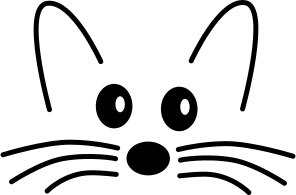
\includegraphics[width=1.4em]{squeak-logo}}}
\newcommand{\dothis}[1]{%
	\medskip
	\noindent\dothisicon
	\ifx#1\empty\else\quad\emph{#1}\fi
	\par\smallskip\nopagebreak}
% NB: To use this in an individual chapter, you must set:
%\graphicspath{{figures/} {../figures/}}
% at the head of the chapter.  Don't forget the final /
%=============================================================
%:Reader hints (hint)
%
% Indicates a non-obvious consequence 
\newcommand{\hint}[1]{\vspace{1ex}\noindent\fbox{\textsc{Astuce}} \emph{#1}}
%=================================================================
% graphics for Morphic handles
\newcommand{\grabHandle}{\raisebox{-0.2ex}{
\includegraphics[width=1em]{blackHandle}}}
\newcommand{\moveHandle}{\raisebox{-0.2ex}{
\includegraphics[width=1em]{moveHandle}}}
\newcommand{\debugHandle}{\raisebox{-0.2ex}{
\includegraphics[width=1em]{debugHandle}}}
% squeak-fr (added for Morphic handles)
\newcommand{\rotateHandle}{\raisebox{-0.2ex}{
\includegraphics[width=1em]{rotateHandle}}}
\newcommand{\viewerHandle}{\raisebox{-0.2ex}{
\includegraphics[width=1em]{viewerHandle}}}
% squeak-fr (add cloverHandle to use \clover in QuickTour.tex as alias
% todo 

%=============================================================
%:Highlighting Important stuff (doublebox)
%
% From Seaside book ...
\newsavebox{\SavedText}
\newlength{\InnerBoxRule}\setlength{\InnerBoxRule}{.75\fboxrule}
\newlength{\OuterBoxRule}\setlength{\OuterBoxRule}{1.5\fboxrule}
\newlength{\BoxSeparation}\setlength{\BoxSeparation}{1.5\fboxrule}
\addtolength{\BoxSeparation}{.5pt}
\newlength{\SaveBoxSep}\setlength{\SaveBoxSep}{2\fboxsep}
%
\newenvironment{doublebox}{\begin{lrbox}{\SavedText}
    \begin{minipage}{.75\textwidth}}
    {\end{minipage}\end{lrbox}\begin{center}
    \setlength{\fboxsep}{\BoxSeparation}\setlength{\fboxrule}{\OuterBoxRule}
    \fbox{\setlength{\fboxsep}{\SaveBoxSep}\setlength{\fboxrule}{\InnerBoxRule}%
      \fbox{\usebox{\SavedText}}}
  \end{center}}
% Use this:
%\newcommand{\important}[1]{\begin{doublebox}#1\end{doublebox}}


\newcommand{\important}[1]{
\noindent\rule{\textwidth}{2pt}\par
\textbf{Important!} #1 \par
\noindent\rule{\textwidth}{2pt}}

\newcommand{\note}[1]{
\noindent\rule{\textwidth}{2pt}\par
\noindent\textbf{Note} #1\par
\noindent\rule{\textwidth}{2pt}}

%=============================================================
%:Section depth
\setcounter{secnumdepth}{2}
%% for this to happen start the file with
%\ifx\wholebook\relax\else
%% $Author$ Martial
% $Date$ Wed Oct 10 13:34:55 CEST 2007
% $Revision$ source: SBE 12715 
% Last Changed Date: 2007-10-08 21:32:45 +0200 (Mon, 08 Oct 2007)
%=============================================================
% NB: documentclass must be set in main document.
% Allows book to be generated in multiple formats.
%=============================================================
%:Packages
%\usepackage[french]{babel}
\usepackage[T1]{fontenc}  %%%%%% really important to get the code directly in the text!
\usepackage{lmodern}
%\usepackage[scaled=0.85]{bookmanx} % needs another scale factor if used with \renewcommand{\sfdefault}{cmbr}
\usepackage{palatino}
%\usepackage[sc]{mathpazo}
%\linespread{1.05}
\usepackage[scaled=0.85]{helvet}
\usepackage{microtype}
\usepackage{graphicx}
\usepackage{theorem}
\usepackage[utf8]{inputenc}
% ON: pdfsync breaks the use of p{width} for tabular columns!
\ifdefined\usepdfsync\usepackage{pdfsync}\fi % Requires texlive 2007
%=============================================================
%:More packages
%Stef should check which ones are used!
%\usepackage{picinpar}
%\usepackage{layout}
%\usepackage{color}
%\definecolor{stefgris}{rgb}{0.85,0.85,0.85}
%\usepackage{enum}
%\usepackage{a4wide}
% \usepackage{fancyhdr}
\usepackage{ifthen}
\usepackage{float}
\usepackage{longtable}
\usepackage{makeidx}
\usepackage[nottoc]{tocbibind}
\usepackage{multicol}
\usepackage{booktabs}	% book-style tables
\usepackage{topcapt}	% enables \topcaption
\usepackage{multirow}
\usepackage{tabularx}
%\usepackage[bottom]{footmisc}
\usepackage{xspace}
\usepackage{alltt}
\usepackage{amssymb,textcomp}
\usepackage[usenames,dvipsnames]{color}
\usepackage{colortbl}
\usepackage[hang]{subfigure}\makeatletter\def\p@subfigure{\thefigure\,}\makeatother
\usepackage{rotating}
\usepackage{enumitem}	% apb: allows more control over tags in enumerations
\usepackage{verbatim}     % for comment environment
\usepackage{varioref}	% for page references that work
\labelformat{footnote}{\thechapter--#1} % to distinguish citations from jurabib
\usepackage{needspace}
\usepackage{isodateo} % enable \isodate
\usepackage[newparttoc]{titlesec}
\usepackage{titletoc}
\usepackage{eurosym}
\usepackage{wrapfig}

\usepackage[
	super,
	citefull=first,
	authorformat={allreversed,and},
	titleformat={commasep,italic}
]{jurabib} % citations as footnotes
\usepackage[
	colorlinks=true,
	linkcolor=black,
	urlcolor=black,
	citecolor=black
]{hyperref}   % should come last

%=============================================================
%:URL style
\makeatletter

\def\url@leostyle{%
  \@ifundefined{selectfont}{\def\UrlFont{\sf}}{\def\UrlFont{\sffamily}}}
% ajouter par Martial pour \traduit (met une dague dans les \doublebox
\def\thempfootnote{\fnsymbol{mpfootnote}}

\makeatother
% Now actually use the newly defined style.
\urlstyle{leo}
%=============================================================
%:Booleans
\newboolean{lulu}
\setboolean{lulu}{false}
\newcommand{\ifluluelse}[2]{\ifthenelse{\boolean{lulu}}{#1}{#2}}
%=============================================================
%:Names
\newcommand{\SUnit}{SUnit\xspace}
\newcommand{\sunit}{SUnit\xspace}
\newcommand{\xUnit}{$x$Unit\xspace}
\newcommand{\JUnit}{JUnit\xspace}
%\newcommand{\XP}{eXtreme Programming\xspace}
\newcommand{\st}{Smalltalk\xspace}
\newcommand{\Squeak}{Squeak\xspace}
\newcommand{\sq}{Squeak\xspace}
\newcommand{\sqmap}{SqueakMap\xspace}
\newcommand{\squeak}{Squeak\xspace}
%\newcommand{\sbe}{\url{scg.unibe.ch/SBE}\xspace}
%\newcommand{\sbe}{\url{squeakbyexample.org}\xspace}
\newcommand{\sbe}{\url{SqueakByExample.org}\xspace}
% squeak-fr: adresse de la version francaise
\newcommand{\spe}{\url{SqueakByExample.org/fr}\xspace}
\newcommand{\sba}{\url{SquareBracketAssociates.org}\xspace}

% squeak-fr: ajout de la \squeakdev pour eviter les problemes de
% changements d'url rencontres dans la VO:
\newcommand{\squeakdev}{\url{www.squeaksource.com/ImageForDevelopers}\xspace} %ou
%\newcommand{\squeakdev}{\url{squeak.ofset.org/squeak-dev}\xspace}

%=============================================================
%:Editorial comment macros
\newcommand{\nnbb}[2]{
    \fbox{\bfseries\sffamily\scriptsize#1}
    {\sf\small$\blacktriangleright$\textit{#2}$\blacktriangleleft$}
   }
\newcommand{\ab}[1]{\nnbb{Andrew}{#1}}
\newcommand{\sd}[1]{\nnbb{St\'{e}f}{#1}}
\newcommand{\md}[1]{\nnbb{Marcus}{#1}}
\newcommand{\on}[1]{\nnbb{Oscar}{#1}}
\newcommand{\damien}[1]{\nnbb{Damien}{#1}}
\newcommand{\lr}[1]{\nnbb{Lukas}{#1}}
\newcommand{\orla}[1]{\nnbb{Orla}{#1}}
%\newcommand{\here}{\nnbb{CONTINUE}{HERE}}
\newcommand{\here}{\nnbb{CONTINUE}{ICI}}

%=============================================================
%:Abbreviation macros
\newcommand{\ie}{\emph{c-\`a-d.}\xspace}
\newcommand{\cad}{\emph{c-\`a-d.}\xspace}
%\newcommand{\eg}{\emph{e.g.},\xspace}
\newcommand{\eg}{\emph{par ex.},\xspace}
\newcommand{\parex}{\emph{par ex.},\xspace}
\newcommand{\etc}{etc\xspace}
%=============================================================
%:Cross reference macros

% [squeak-fr] martial: remarquez les articles devant les noms
\newcommand{\charef}[1]{le chapitre~\ref{cha:#1}\xspace}
% note de martial: utilise dans chapitre Syntax.tex: a redefinir
\newcommand{\charefs}[2]{les chapitres~\ref{cha:#1} et \ref{cha:#2}\xspace}
\newcommand{\secref}[1]{la section~\ref{sec:#1}\xspace}
\newcommand{\figref}[1]{la figure~\ref{fig:#1}\xspace}
\newcommand{\Figref}[1]{La figure~\ref{fig:#1}\xspace}
\newcommand{\appref}[1]{l'annexe~\ref{app:#1}\xspace}
\newcommand{\tabref}[1]{la table~\ref{tab:#1}\xspace}
% defini pour le chapitre Messages.tex
\newcommand{\Tabref}[1]{La table~\ref{tab:#1}\xspace}

% APB: I removed trailing \xspace commands from these macros because
% \xspace mostly doesn't work.  If you want a space after your
% references, type one!
% ON: xspace has always worked just fine for me!  Please leave them in.
%
\newcommand{\ruleref}[1]{\ref{rule:#1}\xspace}
%
\newcommand{\egref}[1]{exemple~\ref{eg:#1}\xspace}
\newcommand{\Egref}[1]{Exemple~\ref{eg:#1}\xspace}
%
\newcommand{\scrref}[1]{script~\ref{scr:#1}\xspace}
\newcommand{\Scrref}[1]{Script~\ref{scr:#1}\xspace}
% t = the
\newcommand{\tscrref}[1]{le script~\ref{scr:#1}\xspace}
\newcommand{\Tscrref}[1]{Le script~\ref{scr:#1}\xspace}
%
\newcommand{\mthref}[1]{m\'ethode~\ref{mth:#1}\xspace}
\newcommand{\mthsref}[1]{m\'ethodes~\ref{mth:#1}\xspace}
\newcommand{\Mthref}[1]{M\'ethode~\ref{mth:#1}\xspace}
\newcommand{\tmthref}[1]{la m\'ethode~\ref{mth:#1}\xspace}
\newcommand{\Tmthref}[1]{La m\'ethode~\ref{mth:#1}\xspace}
%
\newcommand{\clsref}[1]{classe~\ref{cls:#1}\xspace}
\newcommand{\tclsref}[1]{la classe~\ref{cls:#1}\xspace}
\newcommand{\Tclsref}[1]{La classe~\ref{cls:#1}\xspace}
%=============================================================
%:Menu item macro
% for menu items, so we can change our minds on how to print them! (apb)
\definecolor{lightgray}{gray}{0.89}
\newcommand{\menu}[1]{{%
	\setlength{\fboxsep}{0pt}%
	\colorbox{lightgray}{{{\upshape\sffamily\strut \,#1\,}}}}}
% \newcommand{\menu}[1]{{%
% 	\fontfamily{lmr}\selectfont
% 	\upshape\textlangle{\sffamily #1}\textrangle}}
% For submenu items:
\newcommand{\go}{\,$\triangleright$\,}
% \newcommand{\go}{\,$\blacktriangleright$\,}
% For keyboard shortcuts:
%\newcommand{\short}[1]{\mbox{$\langle${\sc CMD}$\rangle$-#1}\xspace}
\newcommand{\short}[1]{\mbox{{\sc cmd}\hspace{0.08em}--\hspace{0.09em}#1}\xspace}
% For buttons:
\newcommand{\button}[1]{{%
	\setlength{\fboxsep}{0pt}%
	\fbox{{\upshape\sffamily\strut \,#1\,}}}}
\newcommand{\toolsflap}{l'onglet \textit{Tools}\xspace}
%=============================================================
%:Reader cues (do this)
%
% Indicate something the reader should try out.
\newcommand{\dothisicon}{\raisebox{-.5ex}{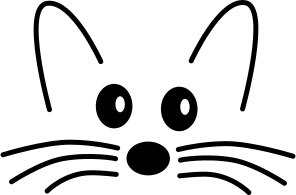
\includegraphics[width=1.4em]{squeak-logo}}}
\newcommand{\dothis}[1]{%
	\medskip
	\noindent\dothisicon
	\ifx#1\empty\else\quad\emph{#1}\fi
	\par\smallskip\nopagebreak}
% NB: To use this in an individual chapter, you must set:
%\graphicspath{{figures/} {../figures/}}
% at the head of the chapter.  Don't forget the final /
%=============================================================
%:Reader hints (hint)
%
% Indicates a non-obvious consequence 
\newcommand{\hint}[1]{\vspace{1ex}\noindent\fbox{\textsc{Astuce}} \emph{#1}}
%=================================================================
% graphics for Morphic handles
\newcommand{\grabHandle}{\raisebox{-0.2ex}{
\includegraphics[width=1em]{blackHandle}}}
\newcommand{\moveHandle}{\raisebox{-0.2ex}{
\includegraphics[width=1em]{moveHandle}}}
\newcommand{\debugHandle}{\raisebox{-0.2ex}{
\includegraphics[width=1em]{debugHandle}}}
% squeak-fr (added for Morphic handles)
\newcommand{\rotateHandle}{\raisebox{-0.2ex}{
\includegraphics[width=1em]{rotateHandle}}}
\newcommand{\viewerHandle}{\raisebox{-0.2ex}{
\includegraphics[width=1em]{viewerHandle}}}
% squeak-fr (add cloverHandle to use \clover in QuickTour.tex as alias
% todo 

%=============================================================
%:Highlighting Important stuff (doublebox)
%
% From Seaside book ...
\newsavebox{\SavedText}
\newlength{\InnerBoxRule}\setlength{\InnerBoxRule}{.75\fboxrule}
\newlength{\OuterBoxRule}\setlength{\OuterBoxRule}{1.5\fboxrule}
\newlength{\BoxSeparation}\setlength{\BoxSeparation}{1.5\fboxrule}
\addtolength{\BoxSeparation}{.5pt}
\newlength{\SaveBoxSep}\setlength{\SaveBoxSep}{2\fboxsep}
%
\newenvironment{doublebox}{\begin{lrbox}{\SavedText}
    \begin{minipage}{.75\textwidth}}
    {\end{minipage}\end{lrbox}\begin{center}
    \setlength{\fboxsep}{\BoxSeparation}\setlength{\fboxrule}{\OuterBoxRule}
    \fbox{\setlength{\fboxsep}{\SaveBoxSep}\setlength{\fboxrule}{\InnerBoxRule}%
      \fbox{\usebox{\SavedText}}}
  \end{center}}
% Use this:
%\newcommand{\important}[1]{\begin{doublebox}#1\end{doublebox}}


\newcommand{\important}[1]{
\noindent\rule{\textwidth}{2pt}\par
\textbf{Important!} #1 \par
\noindent\rule{\textwidth}{2pt}}

\newcommand{\note}[1]{
\noindent\rule{\textwidth}{2pt}\par
\noindent\textbf{Note} #1\par
\noindent\rule{\textwidth}{2pt}}

%=============================================================
%:Section depth
\setcounter{secnumdepth}{2}
%% for this to happen start the file with
%\ifx\wholebook\relax\else
%% $Author$ Martial
% $Date$ Wed Oct 10 13:34:55 CEST 2007
% $Revision$ source: SBE 12715 
% Last Changed Date: 2007-10-08 21:32:45 +0200 (Mon, 08 Oct 2007)
%=============================================================
% NB: documentclass must be set in main document.
% Allows book to be generated in multiple formats.
%=============================================================
%:Packages
%\usepackage[french]{babel}
\usepackage[T1]{fontenc}  %%%%%% really important to get the code directly in the text!
\usepackage{lmodern}
%\usepackage[scaled=0.85]{bookmanx} % needs another scale factor if used with \renewcommand{\sfdefault}{cmbr}
\usepackage{palatino}
%\usepackage[sc]{mathpazo}
%\linespread{1.05}
\usepackage[scaled=0.85]{helvet}
\usepackage{microtype}
\usepackage{graphicx}
\usepackage{theorem}
\usepackage[utf8]{inputenc}
% ON: pdfsync breaks the use of p{width} for tabular columns!
\ifdefined\usepdfsync\usepackage{pdfsync}\fi % Requires texlive 2007
%=============================================================
%:More packages
%Stef should check which ones are used!
%\usepackage{picinpar}
%\usepackage{layout}
%\usepackage{color}
%\definecolor{stefgris}{rgb}{0.85,0.85,0.85}
%\usepackage{enum}
%\usepackage{a4wide}
% \usepackage{fancyhdr}
\usepackage{ifthen}
\usepackage{float}
\usepackage{longtable}
\usepackage{makeidx}
\usepackage[nottoc]{tocbibind}
\usepackage{multicol}
\usepackage{booktabs}	% book-style tables
\usepackage{topcapt}	% enables \topcaption
\usepackage{multirow}
\usepackage{tabularx}
%\usepackage[bottom]{footmisc}
\usepackage{xspace}
\usepackage{alltt}
\usepackage{amssymb,textcomp}
\usepackage[usenames,dvipsnames]{color}
\usepackage{colortbl}
\usepackage[hang]{subfigure}\makeatletter\def\p@subfigure{\thefigure\,}\makeatother
\usepackage{rotating}
\usepackage{enumitem}	% apb: allows more control over tags in enumerations
\usepackage{verbatim}     % for comment environment
\usepackage{varioref}	% for page references that work
\labelformat{footnote}{\thechapter--#1} % to distinguish citations from jurabib
\usepackage{needspace}
\usepackage{isodateo} % enable \isodate
\usepackage[newparttoc]{titlesec}
\usepackage{titletoc}
\usepackage{eurosym}
\usepackage{wrapfig}

\usepackage[
	super,
	citefull=first,
	authorformat={allreversed,and},
	titleformat={commasep,italic}
]{jurabib} % citations as footnotes
\usepackage[
	colorlinks=true,
	linkcolor=black,
	urlcolor=black,
	citecolor=black
]{hyperref}   % should come last

%=============================================================
%:URL style
\makeatletter

\def\url@leostyle{%
  \@ifundefined{selectfont}{\def\UrlFont{\sf}}{\def\UrlFont{\sffamily}}}
% ajouter par Martial pour \traduit (met une dague dans les \doublebox
\def\thempfootnote{\fnsymbol{mpfootnote}}

\makeatother
% Now actually use the newly defined style.
\urlstyle{leo}
%=============================================================
%:Booleans
\newboolean{lulu}
\setboolean{lulu}{false}
\newcommand{\ifluluelse}[2]{\ifthenelse{\boolean{lulu}}{#1}{#2}}
%=============================================================
%:Names
\newcommand{\SUnit}{SUnit\xspace}
\newcommand{\sunit}{SUnit\xspace}
\newcommand{\xUnit}{$x$Unit\xspace}
\newcommand{\JUnit}{JUnit\xspace}
%\newcommand{\XP}{eXtreme Programming\xspace}
\newcommand{\st}{Smalltalk\xspace}
\newcommand{\Squeak}{Squeak\xspace}
\newcommand{\sq}{Squeak\xspace}
\newcommand{\sqmap}{SqueakMap\xspace}
\newcommand{\squeak}{Squeak\xspace}
%\newcommand{\sbe}{\url{scg.unibe.ch/SBE}\xspace}
%\newcommand{\sbe}{\url{squeakbyexample.org}\xspace}
\newcommand{\sbe}{\url{SqueakByExample.org}\xspace}
% squeak-fr: adresse de la version francaise
\newcommand{\spe}{\url{SqueakByExample.org/fr}\xspace}
\newcommand{\sba}{\url{SquareBracketAssociates.org}\xspace}

% squeak-fr: ajout de la \squeakdev pour eviter les problemes de
% changements d'url rencontres dans la VO:
\newcommand{\squeakdev}{\url{www.squeaksource.com/ImageForDevelopers}\xspace} %ou
%\newcommand{\squeakdev}{\url{squeak.ofset.org/squeak-dev}\xspace}

%=============================================================
%:Editorial comment macros
\newcommand{\nnbb}[2]{
    \fbox{\bfseries\sffamily\scriptsize#1}
    {\sf\small$\blacktriangleright$\textit{#2}$\blacktriangleleft$}
   }
\newcommand{\ab}[1]{\nnbb{Andrew}{#1}}
\newcommand{\sd}[1]{\nnbb{St\'{e}f}{#1}}
\newcommand{\md}[1]{\nnbb{Marcus}{#1}}
\newcommand{\on}[1]{\nnbb{Oscar}{#1}}
\newcommand{\damien}[1]{\nnbb{Damien}{#1}}
\newcommand{\lr}[1]{\nnbb{Lukas}{#1}}
\newcommand{\orla}[1]{\nnbb{Orla}{#1}}
%\newcommand{\here}{\nnbb{CONTINUE}{HERE}}
\newcommand{\here}{\nnbb{CONTINUE}{ICI}}

%=============================================================
%:Abbreviation macros
\newcommand{\ie}{\emph{c-\`a-d.}\xspace}
\newcommand{\cad}{\emph{c-\`a-d.}\xspace}
%\newcommand{\eg}{\emph{e.g.},\xspace}
\newcommand{\eg}{\emph{par ex.},\xspace}
\newcommand{\parex}{\emph{par ex.},\xspace}
\newcommand{\etc}{etc\xspace}
%=============================================================
%:Cross reference macros

% [squeak-fr] martial: remarquez les articles devant les noms
\newcommand{\charef}[1]{le chapitre~\ref{cha:#1}\xspace}
% note de martial: utilise dans chapitre Syntax.tex: a redefinir
\newcommand{\charefs}[2]{les chapitres~\ref{cha:#1} et \ref{cha:#2}\xspace}
\newcommand{\secref}[1]{la section~\ref{sec:#1}\xspace}
\newcommand{\figref}[1]{la figure~\ref{fig:#1}\xspace}
\newcommand{\Figref}[1]{La figure~\ref{fig:#1}\xspace}
\newcommand{\appref}[1]{l'annexe~\ref{app:#1}\xspace}
\newcommand{\tabref}[1]{la table~\ref{tab:#1}\xspace}
% defini pour le chapitre Messages.tex
\newcommand{\Tabref}[1]{La table~\ref{tab:#1}\xspace}

% APB: I removed trailing \xspace commands from these macros because
% \xspace mostly doesn't work.  If you want a space after your
% references, type one!
% ON: xspace has always worked just fine for me!  Please leave them in.
%
\newcommand{\ruleref}[1]{\ref{rule:#1}\xspace}
%
\newcommand{\egref}[1]{exemple~\ref{eg:#1}\xspace}
\newcommand{\Egref}[1]{Exemple~\ref{eg:#1}\xspace}
%
\newcommand{\scrref}[1]{script~\ref{scr:#1}\xspace}
\newcommand{\Scrref}[1]{Script~\ref{scr:#1}\xspace}
% t = the
\newcommand{\tscrref}[1]{le script~\ref{scr:#1}\xspace}
\newcommand{\Tscrref}[1]{Le script~\ref{scr:#1}\xspace}
%
\newcommand{\mthref}[1]{m\'ethode~\ref{mth:#1}\xspace}
\newcommand{\mthsref}[1]{m\'ethodes~\ref{mth:#1}\xspace}
\newcommand{\Mthref}[1]{M\'ethode~\ref{mth:#1}\xspace}
\newcommand{\tmthref}[1]{la m\'ethode~\ref{mth:#1}\xspace}
\newcommand{\Tmthref}[1]{La m\'ethode~\ref{mth:#1}\xspace}
%
\newcommand{\clsref}[1]{classe~\ref{cls:#1}\xspace}
\newcommand{\tclsref}[1]{la classe~\ref{cls:#1}\xspace}
\newcommand{\Tclsref}[1]{La classe~\ref{cls:#1}\xspace}
%=============================================================
%:Menu item macro
% for menu items, so we can change our minds on how to print them! (apb)
\definecolor{lightgray}{gray}{0.89}
\newcommand{\menu}[1]{{%
	\setlength{\fboxsep}{0pt}%
	\colorbox{lightgray}{{{\upshape\sffamily\strut \,#1\,}}}}}
% \newcommand{\menu}[1]{{%
% 	\fontfamily{lmr}\selectfont
% 	\upshape\textlangle{\sffamily #1}\textrangle}}
% For submenu items:
\newcommand{\go}{\,$\triangleright$\,}
% \newcommand{\go}{\,$\blacktriangleright$\,}
% For keyboard shortcuts:
%\newcommand{\short}[1]{\mbox{$\langle${\sc CMD}$\rangle$-#1}\xspace}
\newcommand{\short}[1]{\mbox{{\sc cmd}\hspace{0.08em}--\hspace{0.09em}#1}\xspace}
% For buttons:
\newcommand{\button}[1]{{%
	\setlength{\fboxsep}{0pt}%
	\fbox{{\upshape\sffamily\strut \,#1\,}}}}
\newcommand{\toolsflap}{l'onglet \textit{Tools}\xspace}
%=============================================================
%:Reader cues (do this)
%
% Indicate something the reader should try out.
\newcommand{\dothisicon}{\raisebox{-.5ex}{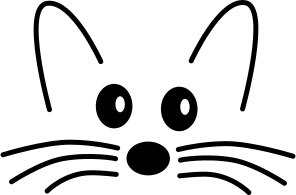
\includegraphics[width=1.4em]{squeak-logo}}}
\newcommand{\dothis}[1]{%
	\medskip
	\noindent\dothisicon
	\ifx#1\empty\else\quad\emph{#1}\fi
	\par\smallskip\nopagebreak}
% NB: To use this in an individual chapter, you must set:
%\graphicspath{{figures/} {../figures/}}
% at the head of the chapter.  Don't forget the final /
%=============================================================
%:Reader hints (hint)
%
% Indicates a non-obvious consequence 
\newcommand{\hint}[1]{\vspace{1ex}\noindent\fbox{\textsc{Astuce}} \emph{#1}}
%=================================================================
% graphics for Morphic handles
\newcommand{\grabHandle}{\raisebox{-0.2ex}{
\includegraphics[width=1em]{blackHandle}}}
\newcommand{\moveHandle}{\raisebox{-0.2ex}{\includegraphics[width=1em]{moveHandle}}}
\newcommand{\debugHandle}{\raisebox{-0.2ex}{\includegraphics[width=1em]{debugHandle}}}
% squeak-fr (added for Morphic handles)
\newcommand{\rotateHandle}{\raisebox{-0.2ex}{\includegraphics[width=1em]{rotateHandle}}}
\newcommand{\viewerHandle}{\raisebox{-0.2ex}{\includegraphics[width=1em]{viewerHandle}}}
% squeak-fr (add cloverHandle to use \clover in QuickTour.tex as alias
% todo 

%=============================================================
%:Highlighting Important stuff (doublebox)
%
% From Seaside book ...
\newsavebox{\SavedText}
\newlength{\InnerBoxRule}\setlength{\InnerBoxRule}{.75\fboxrule}
\newlength{\OuterBoxRule}\setlength{\OuterBoxRule}{1.5\fboxrule}
\newlength{\BoxSeparation}\setlength{\BoxSeparation}{1.5\fboxrule}
\addtolength{\BoxSeparation}{.5pt}
\newlength{\SaveBoxSep}\setlength{\SaveBoxSep}{2\fboxsep}
%
\newenvironment{doublebox}{\begin{lrbox}{\SavedText}
    \begin{minipage}{.75\textwidth}}
    {\end{minipage}\end{lrbox}\begin{center}
    \setlength{\fboxsep}{\BoxSeparation}\setlength{\fboxrule}{\OuterBoxRule}
    \fbox{\setlength{\fboxsep}{\SaveBoxSep}\setlength{\fboxrule}{\InnerBoxRule}%
      \fbox{\usebox{\SavedText}}}
  \end{center}}
% Use this:
%\newcommand{\important}[1]{\begin{doublebox}#1\end{doublebox}}


\newcommand{\important}[1]{
\noindent\rule{\textwidth}{2pt}\par
\textbf{Important!} #1 \par
\noindent\rule{\textwidth}{2pt}}

\newcommand{\note}[1]{
\noindent\rule{\textwidth}{2pt}\par
\noindent\textbf{Note} #1\par
\noindent\rule{\textwidth}{2pt}}

%=============================================================
%:Section depth
\setcounter{secnumdepth}{2}
%% for this to happen start the file with
%\ifx\wholebook\relax\else
%\input{../common.tex}
%\begin{document}
%\fi
% and terminate by
% \ifx\wholebook\relax\else\end{document}\fi

\DeclareGraphicsExtensions{.pdf, .jpg, .png}
%=============================================================
%:PDF setup
\hypersetup{
%   a4paper,
%   pdfstartview=FitV,
%   colorlinks,
%   linkcolor=darkblue,
%   citecolor=darkblue,
%   pdftitle={Squeak by Example},
pdftitle={Squeak par l'exemple},
   pdfauthor={Andrew Black, St\'ephane Ducasse,	Oscar Nierstrasz,
Damien Pollet},
   pdfkeywords={Smalltalk, Squeak, Programmation Orient\'ee Objet},
pdfsubject={Informatique, Computer Science}
}
%=============================================================
%:Page layout and appearance
%
% \renewcommand{\headrulewidth}{0pt}
\renewcommand{\chaptermark}[1]{\markboth{#1}{}}
\renewcommand{\sectionmark}[1]{\markright{\thesection\ #1}}
\renewpagestyle{plain}[\small\itshape]{%
	\setheadrule{0pt}%
	\sethead[][][]{}{}{}%
	\setfoot[][][]{}{}{}}
\renewpagestyle{headings}[\small\itshape]{%
	\setheadrule{0pt}%
	\setmarks{chapter}{section}%
	\sethead[\thepage][][\chaptertitle]{\sectiontitle}{}{\thepage}%
	\setfoot[][][]{}{}{}}
% pagestyle for tableofcontents + index (martial: 2008/04/23)
\newpagestyle{newheadings}[\small\itshape]{%
	\setheadrule{0pt}%
	\setmarks{chapter}{section}%
	\sethead[\thepage][][\chaptertitle]{\chaptertitle}{}{\thepage}%
	\setfoot[][][]{}{}{}}
%=============================================================
%:Title section setup and TOC numbering depth
\setcounter{secnumdepth}{1}
\setcounter{tocdepth}{1}
\titleformat{\part}[display]{\centering}{\huge\partname\ \thepart}{1em}{\Huge\textbf}[]
\titleformat{\chapter}[display]{}{\huge\chaptertitlename\ \thechapter}{1em}{\Huge\raggedright\textbf}[]
\titlecontents{part}[3pc]{%
		\pagebreak[2]\addvspace{1em plus.4em minus.2em}%
		\leavevmode\large\bfseries}
	{\contentslabel{3pc}}{\hspace*{-3pc}}
	{}[\nopagebreak]
\titlecontents{chapter}[3pc]{%
		\pagebreak[0]\addvspace{1em plus.2em minus.2em}%
		\leavevmode\bfseries}
	{\contentslabel{3pc}}{}
	{\hfill\contentspage}[\nopagebreak]
\dottedcontents{section}[3pc]{}{3pc}{1pc}
\dottedcontents{subsection}[3pc]{}{0pc}{1pc}
% \dottedcontents{subsection}[4.5em]{}{0pt}{1pc}
% Make \cleardoublepage insert really blank pages http://www.tex.ac.uk/cgi-bin/texfaq2html?label=reallyblank
\let\origdoublepage\cleardoublepage
\newcommand{\clearemptydoublepage}{%
  \clearpage
  {\pagestyle{empty}\origdoublepage}}
\let\cleardoublepage\clearemptydoublepage % see http://www.tex.ac.uk/cgi-bin/texfaq2html?label=patch
%=============================================================
%:FAQ macros (for FAQ chapter)
\newtheorem{faq}{FAQ}
\newcommand{\answer}{\paragraph{R\'eponse}\ }
%=============================================================
%:Listings package configuration
\usepackage{listings}
\newcommand{\caret}{\makebox{\raisebox{0.4ex}{\footnotesize{$\wedge$}}}}
\lstdefinelanguage{Smalltalk}{
%  morekeywords={self,super,true,false,nil,thisContext}, % This is overkill
  morestring=[d]',
  morecomment=[s]{"}{"},
  alsoletter={\#:},
  escapechar={!},
  escapebegin=\itshape, % comment-like by default (Martial 11/2007)
  literate=
    {BANG}{!}1
    {UNDERSCORE}{\_}1
    {\\st}{Smalltalk}9 % convenience -- in case \st occurs in code
    % {'}{{\textquotesingle}}1 % replaced by upquote=true in \lstset
    {_}{{$\leftarrow$}}1
    {>>>}{{\sep}}1
    {^}{{$\uparrow$}}1
    {~}{{$\sim$}}1
    {-}{{\sf -\hspace{-0.13em}-}}1  % the goal is to make - the same width as +
    {+}{\raisebox{0.08ex}{+}}1		% and to raise + off the baseline to match -
    {-->}{{\quad$\longrightarrow$\quad}}3
	, % Don't forget the comma at the end!
  tabsize=4
}[keywords,comments,strings]
% ajout pour les échappements dans les codes
% indispensable pour mettre le code en emphase (cf. Model.tex) 
\newcommand{\codeify}[1]{\NoAutoSpaceBeforeFDP#1\AutoSpaceBeforeFDP}
\newcommand{\normcomment}[1]{\emph{#1}} %cf. Streams
\newcommand{\normcode}[1]{\emph{\codeify{#1}}} %cf. Streams
\newcommand{\emcode}[1]{\textbf{\normcode{#1}}} % Martial 11/2007
\lstset{language=Smalltalk,
	basicstyle=\sffamily,
	keywordstyle=\color{black}\bfseries,
	% stringstyle=\ttfamily, % Ugly! do we really want this? -- on
	%commentstyle=\itshape,
	mathescape=true,
	showstringspaces=false,
	keepspaces=true,
	breaklines=true,
	breakautoindent=true,
	lineskip={-1pt}, % Ugly hack
	upquote=true, % straight quote; requires textcomp package
	columns=fullflexible} % no fixed width fonts
% In-line code (literal)
% Normally use this for all in-line code:
\newcommand{\ct}{\lstinline[mathescape=false,basicstyle={\sffamily\upshape}]}
% apb 2007.8.28 added the \upshape declaration to avoid getting italicized code in \dothis{ } sections.
% In-line code (latex enabled)
% Use this only in special situations where \ct does not work
% (within section headings ...):

% [squeak-fr] Modification de \lct suivant les indications de Martial Boniou
\newcommand{\lct}[1]{\textsf{\textup{\NoAutoSpaceBeforeFDP #1
\AutoSpaceBeforeFDP}}} %\xspace

% Use these for system categories and protocols:
\newcommand{\scat}[1]{\emph{\textsf{#1}}\xspace}
\newcommand{\pkg}[1]{\emph{\textsf{#1}}\xspace}
\newcommand{\prot}[1]{\emph{\textsf{#1}}\xspace}
% Code environments
% NB: the arg is for tests
% Only code and example environments may be tests
\lstnewenvironment{code}[1]{%
	\lstset{%
		frame=lines,
		mathescape=false
	}
}{}
\def\ignoredollar#1{}
%=============================================================
%:Code environments (method, script ...)
% NB: the third arg is for tests
% Only code and example environments may be tests
\lstnewenvironment{example}[3][defaultlabel]{%
	\renewcommand{\lstlistingname}{Exemple}%
	\lstset{
		frame=lines,
		mathescape=false,
		caption={\emph{#2}},
		label={eg:#1}
	}
}{}
\lstnewenvironment{script}[2][defaultlabel]{%
\renewcommand{\lstlistingname}{Script}%
	\lstset{
		frame=lines,
		mathescape=false,
		name={Script},
		caption={\emph{#2}},
		label={scr:#1}
	}
}{}
%I could not find a way yo get the Experiment #numb followed by the caption in a black box
%\colorbox{black}{\makebox[\textwidth]{  \color{white} {\large {\bfseries Experiment 3-1 (crear i moure un robot)}} }}
\lstnewenvironment{experiment}[2][defaultlabel]{%
%\noindent\rule{\textwidth}{2pt}\vspace{-0.8cm}
\renewcommand{\lstlistingname}{Experiment}%
	\lstset{
		frame=none,
		rulecolor=\color{black},
		mathescape=false,
		name={Experiment},
		caption={\emph{#2}},
		label={scr:#1}
	}
}{%\vspace{-0.5cm}\noindent\rule{\textwidth}{2pt}
}

\lstnewenvironment{method}[2][defaultlabel]{%
	\renewcommand{\lstlistingname}{Method}%
	\lstset{
		frame=lines,
		mathescape=false,
		name={M\'ethode},
		caption={\emph{#2}},
		label={mth:#1}
	}
}{}
\lstnewenvironment{methods}[2][defaultlabel]{% just for multiple methods at once
	\renewcommand{\lstlistingname}{Methods}%
	\lstset{
		frame=lines,
		mathescape=false,
		name={M\'ethode},
		caption={\emph{#2}},
		label={mth:#1}
	}
}{}
\lstnewenvironment{numMethod}[2][defaultlabel]{%
	\renewcommand{\lstlistingname}{Method}%
	\lstset{
		numbers=left,
		numberstyle={\tiny\sffamily},
		frame=lines,
		mathescape=false,
		name={M\'ethode},
		caption={\emph{#2}},
		label={mth:#1}
	}
}{}
% \lstnewenvironment{classdef}[2][defaultlabel]{%
% 	\renewcommand{\lstlistingname}{Classe}%
% 	\lstset{
% 		frame=lines,
% 		mathescape=false,
% 		name={Classe},
% 		caption={\emph{#2}},
% 		label={cls:#1}
% 	}
% }{}

%%%%%%%%%%%%%%%%%%%%%%%%%%%%%%%%%%%%%%%%%%%%%%%%%%%%%%%%%%%%%%%%%%%%%%%%%%%%%%%%%%%%%%%%%%%%%%%%%
%%From the original book latex template
%%%%%%%%%%%%%%%%%%%%%%%%%%%%%%%%%%%%%%%%%%%%%%%%%%%%%%%%%%%%%%%%%%%%%%%%%%%%%%%%%%%%%%%%%%%%%%%%%
\theoremstyle{break}
{\theorembodyfont{\rmfamily}\theoremstyle{break}
\newtheorem{privScript}{Script}[chapter]
%\newtheorem{privMethod}{Method}[chapter]
\newtheorem{privExercise}{Experiment}[chapter]}

% \theoremstyle{break}
% {\theorembodyfont{\rmfamily} \newtheorem{privMethod}{Method}[chapter]}

%class
\theoremstyle{break}
{\theorembodyfont{\rmfamily} \newtheorem{privClassDef}{Class}[chapter]}

%important
\theoremstyle{break}
{\theorembodyfont{\rmfamily} \newtheorem{privTemplate}{Important Messages}[chapter]}

% experiment
\newenvironment{exercise}
    {\begin{privExercise}\mbox{}\\}
    {\end{privExercise}}


%%% for figure
\newsavebox{\ScriptFigure}
\newlength{\ScriptWidth}
\newlength{\FigureWidth}

%%%%%%%%%%%%%%%%%%%%%%%%%%%%%%%%%%%%%%%%%%%%%%%%%%%%%%%%%%%%%%%%%%%%%%%%%%%%%%%%
\newenvironment{scriptfig}[3][0.6]
   {\setlength{\ScriptWidth}{\linewidth*\real{#1}}%
   \setlength{\FigureWidth}{\linewidth-(\linewidth*\real{#1})}%
   \savebox{\ScriptFigure}%
	{\parbox{\FigureWidth}{\includegraphics[width=0.98\FigureWidth]{#2}}}%
   \par\noindent\begin{minipage}{\linewidth}\hrule\vskip 0.2cm\begin{minipage}[c]{\ScriptWidth}%
   \begin{stefscript}[{\em #3}]\begin{alltt}\sffamily}
   {\end{alltt}\end{stefscript}\end{minipage}\hfill
   \usebox{\ScriptFigure}
   \vskip 1ex\hrule\end{minipage}\vskip 1ex\par}

%%%%%%%%%%%%%%%%%%%%%%%%%%%%%%%%%%%%%%%%%%%%%%%%%%%%%%%%%%%%%%%%%%%%%%%%%%%%%%%%
%% to be able to specify the complete set of values for includegraphics
%% may be will be changed but not the interface
\newenvironment{scriptfigwithsize}[3][0.6]
   {\setlength{\ScriptWidth}{\linewidth*\real{#1}}%
   \setlength{\FigureWidth}{\linewidth-(\linewidth*\real{#1})}%
   \savebox{\ScriptFigure}{\parbox{\FigureWidth}{\raggedleft{#2}}}%
   \par\noindent\begin{minipage}{\linewidth}\hrule\vskip 0.3cm\begin{minipage}[c]{\ScriptWidth}%
   \begin{stefscript}[{\em #3}]\begin{alltt}\sffamily}
   {\end{alltt}\end{stefscript}\end{minipage}\hfill
   \usebox{\ScriptFigure}
   \vskip 1ex\hrule\end{minipage}\vskip 1ex\par}

% \newenvironment{methodfig}[2][0.6]
%    {\setlength{\ScriptWidth}{\linewidth*\real{#1}}%
%    \setlength{\FigureWidth}{\linewidth-(\linewidth*\real{#1})}%
%    \savebox{\ScriptFigure}{\parbox{\FigureWidth}{\includegraphics[width=.98\FigureWidth]{#2}}}%
%    \par\noindent\rule{\linewidth}{1mm}
%    \\[-0.3cm]\noindent\rule{\linewidth}{0.1mm}
%    \noindent\begin{minipage}[c]{\ScriptWidth}\begin{privMethod}\begin{alltt}\sffamily}
%    {\end{alltt}\end{privMethod}\end{minipage}\hfill
%    \usebox{\ScriptFigure} \vskip 1ex\hrule\vskip 1ex\par}

% \newenvironment{method}
% {\par\noindent\begin{minipage}{\linewidth}\vspace{0.2cm}\begin{privMethod}\begin{nminipage}\vspace{-0.2cm}\rule{\linewidth}{1mm}\\[-0.6cm]\rule{\linewidth}{0.1mm}\end{nminipage}\hspace*{\scriptindent}\codesize\begin{nalltt}\vspace{-0.2cm}}
% {\end{nalltt}\normalsize\vspace{-0.1cm}\hrule\end{privMethod}\vspace{0.2cm}\end{minipage}}


% \newenvironment{classdef}
% {\par\noindent\begin{minipage}{\linewidth}\vspace{0.2cm}\begin{privClassDef}\begin{nminipage}\vspace{-0.2cm}\rule{\linewidth}{1mm}\\[-0.6cm]\rule{\linewidth}{0.1mm}\end{nminipage}\hspace*{\scriptindent}\codesize\begin{nalltt}\vspace{-0.2cm}}
% {\end{nalltt}\normalsize\vspace{-0.1cm}\hrule\end{privClassDef}\vspace{0.2cm}\end{minipage}}


% \newenvironment{template}
% {\par\noindent\begin{minipage}{\linewidth}\vspace{0.3cm}\begin{privTemplate}\begin{nminipage}\vspace{-0.4cm}\rule{\linewidth}{0.1mm}\end{nminipage}\hspace*{\scriptindent}\begin{nalltt}\vspace{-0.7cm}}
% {\end{nalltt}\vspace{-0.1cm}\hrule\end{privTemplate}\end{minipage}\vspace{0.3cm}}

\newenvironment{exofig}[2][0.7]
   {\setlength{\ScriptWidth}{\linewidth*\real{#1}}
   \setlength{\FigureWidth}{\linewidth-(\linewidth*\real{#1})}
   \savebox{\ScriptFigure}{\parbox{\FigureWidth}{\raggedleft{\includegraphics[width=.98\FigureWidth]{#2}}}}
   \par\noindent\begin{minipage}{\linewidth}\hrule\vskip 0.3cm\begin{minipage}[c]{\ScriptWidth}%
   \begin{privExercise}}
   {\end{privExercise}\end{minipage}\hfill
   \usebox{\ScriptFigure}
   \vskip 1ex\hrule\end{minipage}\vskip 1ex\par}

\newenvironment{exofigwithsize}[2][0.7]
   {\setlength{\ScriptWidth}{\linewidth*\real{#1}}
   \setlength{\FigureWidth}{\linewidth-(\linewidth*\real{#1})}
   \savebox{\ScriptFigure}{\parbox{\FigureWidth}{\raggedleft{#2}}}
   \par\noindent\begin{minipage}{\linewidth}\hrule\vskip 0.3cm\begin{minipage}[c]{\ScriptWidth}%
   \begin{privExercise}}
   {\end{privExercise}\end{minipage}\hfill\usebox{\ScriptFigure}
   \vskip 1ex\hrule\end{minipage}\vskip 1ex\par}

\newenvironment{exofigwithsizeandtitle}[3][0.7]
   {\setlength{\ScriptWidth}{\linewidth*\real{#1}}
   \setlength{\FigureWidth}{\linewidth-(\linewidth*\real{#1})}
   \savebox{\ScriptFigure}{\parbox{\FigureWidth}{\raggedleft{#2}}}
   \vskip 0.3cm\par\noindent\begin{minipage}{\linewidth}\hrule\vskip 0.1cm\begin{minipage}[c]{\ScriptWidth}%
   \begin{privExercise}[\em{#3}]}
   {\end{privExercise}\end{minipage}\hfill\usebox{\ScriptFigure}
   \vskip 1ex\hrule\end{minipage}\vskip 1ex\par}

\newenvironment{exofigwithtitle}[3][0.7]
   {\setlength{\ScriptWidth}{\linewidth*\real{#1}}
   \setlength{\FigureWidth}{\linewidth-(\linewidth*\real{#1})}
   \savebox{\ScriptFigure}{\parbox{\FigureWidth}{\raggedleft{\includegraphics[width=.98\FigureWidth]{#2}}}}
   \par\noindent\begin{minipage}{\linewidth}\hrule\vskip 0.3cm\begin{minipage}[c]{\ScriptWidth}%
   \begin{privExercise}[\em{#3}]}
   {\end{privExercise}\end{minipage}\hfill
   \usebox{\ScriptFigure}
   \vskip 1ex\hrule\end{minipage}\vskip 1ex\par}


\newenvironment{exonofigwithtitle}[3][0.7]
   {\setlength{\ScriptWidth}{\linewidth*\real{#1}}
   \setlength{\FigureWidth}{\linewidth-(\linewidth*\real{#1})}
   \savebox{\ScriptFigure}{\parbox{\FigureWidth}{\raggedleft{\includegraphics[width=.98\FigureWidth]{#2}}}}
   \par\noindent\begin{minipage}{\linewidth}\hrule\vskip 0.3cm\begin{minipage}[c]{\ScriptWidth}%
   \begin{privExercise}[\em{#3}]}
   {\end{privExercise}\end{minipage}\hfill
   \usebox{\ScriptFigure}
   \vskip 1ex\hrule\end{minipage}\vskip 1ex\par}

\newenvironment{exonofig}
   {\par\noindent\begin{minipage}[t]{\linewidth}\noindent\begin{privExercise}}
   {\end{privExercise}\end{minipage}\vspace{0.5cm}\par}

\newenvironment{exonofigtitle}[1]
   {\par\noindent\begin{minipage}[t]{\linewidth}\noindent\begin{privExercise}[\em{#1}]}
   {\end{privExercise}\end{minipage}\vspace{0.5cm}\par}
		
% \newenvironment{solfig}[3][0.5]
%    {\setlength{\ScriptWidth}{\linewidth*\real{#1}}
%    \setlength{\FigureWidth}{\linewidth-\linewidth*\real{#1}}
%    \savebox{\ScriptFigure}{\parbox{\FigureWidth}{\includegraphics[width=.9\linewidth]{#2}}}
%    \par\noindent\vskip 1ex\hrule\vskip 1ex\begin{minipage}[t]{\ScriptWidth}
%    {\bf Solution #3} \begin{alltt}\sffamily}
%    {\end{alltt}\end{minipage}\hfill
%    \usebox{\ScriptFigure}
%    \vskip 1ex\hrule\vskip 1ex\par}
% 
% \newenvironment{solnofig}[1]
%    {\par\noindent\vskip 1ex\hrule\vskip 1ex\begin{minipage}[t]{\ScriptWidth}
%    {\bf Solution #1} \begin{alltt}\sffamily}
%    {\end{alltt}\end{minipage}\hfill
%    \vskip 1ex\hrule\vskip 1ex\par}
% 
% \newenvironment{exoscript}[3][0.5]
%    {\setlength{\ScriptWidth}{\linewidth*\real{#1}}
%     \setlength{\FigureWidth}{\linewidth-\linewidth*\real{#1}}
%     \savebox{\ScriptFigure}{\begin{minipage}\begin{alltt}\sffamily#3\end{alltt}\end{minipage}}
%     \par\noindent\vskip 1ex\hrule\vskip 1ex\begin{minipage}[t]{\ScriptWidth}
%     \begin{privExercise}}
%     {\end{privExercise}\end{minipage}\hfill
%     \usebox{\ScriptFigure}
% \vskip 1ex\hrule\vskip 1ex\par}


%%%%%%%%%%%%%%%%%%%%%%%%%%%%%%%%%%%%%%%%%%%%%%%%%%%%%%%%%%%%%%%%
%% Define the indentation from which the code script starts
%\newlength{\scriptindent}
%\setlength{\scriptindent}{.3cm}
%%%%%%%%%%%%%%%%%%%%%%%%%%%%%%%%%%%%%%%%%%%%%%%%%%%%%%%%%%%%%%%%
%% Method presentation 
%\newlength{\methodindent}
%\newlength{\methodwordlength}
%\newlength{\aftermethod}
%\setlength{\methodindent}{0.2cm}
%\settowidth{\methodwordlength}{\ M\'ethode\ }

%%%%%%%%%%%%%%%%%%%%%%%%%%%%%%%%%%%%%%%%%%%%%%%%%%%%%%%%%%%%%%%%
\theoremstyle{break}
{\theorembodyfont{\rmfamily} \newtheorem{fonction}{Script}[chapter]}

\newsavebox{\fminibox}
\newlength{\fminilength}
% Fait un truc encadre
\newenvironment{fminipage}[1][\linewidth]
  {\setlength{\fminilength}{#1-2\fboxsep-2\fboxrule}
        \begin{lrbox}{\fminibox}\begin{minipage}{\fminilength}}
  { \end{minipage}\end{lrbox}\noindent\fbox{\usebox{\fminibox}}}

% Pareil mais pas encadre (a utiliser pour ne pas couper une fonction en 2)
\newenvironment{nminipage}[1][\linewidth]
  {\setlength{\fminilength}{#1}
        \begin{lrbox}{\fminibox}\begin{minipage}{\fminilength}}
  { \end{minipage}\end{lrbox}\noindent\mbox{\usebox{\fminibox}}}

% Un alltt encadre
\newenvironment{falltt}
  {\vspace*{0.3cm}\begin{fminipage}\begin{alltt}\ttfamily}
  {\end{alltt}\end{fminipage}\vspace*{0.3cm}}

% Un alltt pas encadre
\newenvironment{nalltt}
  {\vspace*{0.3cm}\begin{nminipage}\begin{alltt}\sffamily}
  {\end{alltt}\end{nminipage}\vspace*{0.3cm}}

% Une fonction encadree
\newenvironment{ffonction}[1]
  {\begin{fonction}[#1]\begin{fminipage}\begin{alltt}\ttfamily\rule{\linewidth}{0.5pt}}
{\end{alltt}\end{fminipage}\end{fonction}}


\theoremstyle{break}
{\theorembodyfont{\rmfamily} \newtheorem{stefscript}{Script}[chapter]}

\theoremstyle{break}
{\theorembodyfont{\rmfamily} \newtheorem{exampleScript}{Examples}[chapter]}


%%Not used
\newenvironment{ncscript}[1]
{\vspace{-0.5cm}\begin{stefscript}[#1]\begin{nalltt}\rule{\linewidth}{1.5pt}\vspace{-0.1cm}
\hspace*{\scriptindent}\begin{nalltt}}
{\end{nalltt}\vspace{-0.5cm}\hrule\end{nalltt}\end{stefscript}\vspace{-0.5cm}}
%%Not used
\newenvironment{soluscript}[1]
{\begin{nalltt}\textbf{Solution du script : #1.}\\
\rule{\linewidth}{1.5pt}
\hspace*{\scriptindent}\begin{nalltt}}
{\end{nalltt}\vspace{-0.5cm}\hrule\end{nalltt}\vspace{-0.5cm}\\}




\newenvironment{scriptwithtitle}[1]
{\vspace{-0.3cm}\begin{stefscript}[{\em #1}]\begin{nalltt}\rule{\linewidth}{1.5pt}\vspace{-0.3cm}\hspace*{\scriptindent}\begin{nalltt}\codesize}
{\normalsize\end{nalltt}\vspace{-0.2cm}\hrule\end{nalltt}\end{stefscript}\vspace{-0.5cm}}

\newenvironment{scriptwithouttitle}
{\vspace{-0.5cm}\begin{stefscript}\codesize\begin{nalltt}\rule{\linewidth}{1.5pt}\vspace{-0.1cm}
\hspace*{\scriptindent}\begin{nalltt}}
{\end{nalltt}\vspace{-0.5cm}\hrule\end{nalltt}\normalsize\end{stefscript}\vspace{-0.5cm}}

% \newenvironment{example}
% {\vspace{-0.5cm}\begin{exampleScript}\codesize\begin{nalltt}\rule{\linewidth}{1.5pt}\vspace{-0.1cm}\hspace*{\scriptindent}\begin{nalltt}}
% {\end{nalltt}\vspace{-0.2cm}\hrule\end{nalltt}\normalsize\end{exampleScript}\vspace{-0.5cm}}




























%=============================================================
%:Reserving space
% Usually need one more line than the actual lines of code
\newcommand{\needlines}[1]{\Needspace{#1\baselineskip}}
%=============================================================
%:Indexing macros
% Macros ending with "ind" generate text as well as an index entry
% Macros ending with "index" *only* generate an index entry
\newcommand{\ind}[1]{\index{#1}#1\xspace} % plain text
\newcommand{\subind}[2]{\index{#1!#2}#2\xspace} % show #2, subindex inder #1
\newcommand{\emphind}[1]{\index{#1}\emph{#1}\xspace} % emph #1
\newcommand{\emphsubind}[2]{\index{#1!#2}\emph{#2}\xspace} % show emph #2, subindex inder #1
\newcommand{\scatind}[1]{\index{#1@\textsf{#1} (cat\'egorie)}\scat{#1}} % category
\newcommand{\protind}[1]{\index{#1@\textsf{#1} (protocole)}\prot{#1}} % protocol
% \newcommand{\clsind}[1]{\index{#1@\textsf{#1} (class)}\ct{#1}\xspace}
\newcommand{\clsind}[1]{\index{#1!\#@(classe)}\ct{#1}\xspace} % class
\newcommand{\cvind}[1]{\index{#1@\textsf{#1} (variable de classe)}\ct{#1}\xspace} % class var
\newcommand{\glbind}[1]{\index{#1@\textsf{#1} (globale)}\ct{#1}\xspace} % global
\newcommand{\patind}[1]{\index{#1@#1 (patron)}\ct{#1}\xspace} % pattern
\newcommand{\pvind}[1]{\index{#1@\textsf{#1} (pseudo-variable)}\ct{#1}\xspace} % pseudo variable
% [squeak - fr]Martial: I found the following cleaner (should be
% merged in SBE for self and super)
\newcommand{\subpvindex}[2]{\index{#1@\textsf{#1} (pseudo-variable)!#2}}
\newcommand{\subpvind}[2]{\index{#1@\textsf{#1} (pseudo-variable)!#2}#2\xspace}
% used in Model.tex
\newcommand{\mthind}[2]{\index{#1!#2@\ct{#2}}\ct{#2}\xspace} % show method name only
\newcommand{\lmthind}[2]{\index{#1!#2@\ct{#2}}\lct{#2}\xspace} % show method name only
\newcommand{\cmind}[2]{\index{#1!#2@\ct{#2}}\ct{#1>>>#2}\xspace} % show class>>method
\newcommand{\toolsflapind}{\index{onglet Tools}\toolsflap} % index tools flap
% The following only generate an index entry:
% \newcommand{\clsindex}[1]{\index{#1@\textsf{#1} (class)}}
\newcommand{\clsindex}[1]{\index{#1!\#@(classe)}} % class
\newcommand{\cmindex}[2]{\index{#1!#2@\ct{#2}}} % class>>method
\newcommand{\cvindex}[1]{\index{#1@\textsf{#1} (variable de classe)}} % class var
\newcommand{\glbindex}[1]{\index{#1@\textsf{#1} (globale)}}% global
\newcommand{\pvindex}[1]{\index{#1@\textsf{#1} (pseudo-variable)}}% pseudo var
\newcommand{\seeindex}[2]{\index{#1|see{#2}}} % #1, see #2
\newcommand{\scatindex}[1]{\index{#1@\textsf{#1} (cat\'egorie)}} % category
\newcommand{\protindex}[1]{\index{#1@\textsf{#1} (protocole)}} % protocol
% How can we have the main entry page numbers in bold yet not break the hyperlink?
\newcommand{\boldidx}[1]{{\bf #1}} % breaks hyperlink
%\newcommand{\indmain}[1]{\index{#1|boldidx}#1\xspace} % plain text, main entry
%\newcommand{\emphsubindmain}[2]{\index{#1!#2|boldidx}\emph{#2}\xspace} % subindex, main entry
%\newcommand{\subindmain}[2]{\index{#1!#2|boldidx}#2\xspace} % subindex, main entry
%\newcommand{\clsindmain}[1]{\index{#1@\textsf{#1} (class)|boldidx}\ct{#1}\xspace}
%\newcommand{\clsindmain}[1]{\index{#1!\#@(class)|boldidx}\ct{#1}\xspace} % class main
%\newcommand{\indexmain}[1]{\index{#1|boldidx}} % main index entry only
\newcommand{\indmain}[1]{\index{#1}#1\xspace} 
\newcommand{\emphsubindmain}[2]{\index{#1!#2}\emph{#2}\xspace} % subindex, main entry
\newcommand{\subindmain}[2]{\index{#1!#2}#2\xspace} % subindex, main entry
%\newcommand{\clsindmain}[1]{\index{#1@\textsf{#1} (class)}\ct{#1}\xspace}
\newcommand{\clsindmain}[1]{\index{#1!\#@(classe)}\ct{#1}\xspace} % class main
\newcommand{\indexmain}[1]{\index{#1}} 
%=============================================================
%:Code macros
% some constants
\newcommand{\codesize}{\small}
\newcommand{\codefont}{\sffamily}
\newcommand{\cat}[1]{\textit{Dans la cat\'egorie #1}}%%To remove later
\newlength{\scriptindent}
\setlength{\scriptindent}{.3cm}
%% Method presentation constants
\newlength{\methodindent}
\newlength{\methodwordlength}
\newlength{\aftermethod}
\setlength{\methodindent}{0.2cm}
\settowidth{\methodwordlength}{\ M\'ethode\ }
%=============================================================
%:Smalltalk macros
%\newcommand{\sep}{{$\gg$}}
\newcommand{\sep}{\mbox{>>}}
\newcommand{\self}{\ct{self}\xspace}
\newcommand{\super}{\ct{super}\xspace}
\newcommand{\nil}{\ct{nil}\xspace}
%=============================================================
% be less conservative about float placement
% these commands are from http://www.tex.ac.uk/cgi-bin/texfaq2html?label=floats
\renewcommand{\topfraction}{.9}
\renewcommand{\bottomfraction}{.9}
\renewcommand{\textfraction}{.1}
\renewcommand{\floatpagefraction}{.85}
\renewcommand{\dbltopfraction}{.66}
\renewcommand{\dblfloatpagefraction}{.85}
\setcounter{topnumber}{9}
\setcounter{bottomnumber}{9}
\setcounter{totalnumber}{20}
\setcounter{dbltopnumber}{9}
%=============================================================
%% [Squeak-fr]
% pour identifier les zones de texte à corriger d'urgence!
\newcommand{\arevoir}[1]{#1}
% \traduit utilisé dans Model.tex
\newcommand{\traduit}[1]{\footnote[2]{#1}}
% changeset alias
\newcommand{\changeset}{\emph{change set}\xspace}
\newcommand{\changesets}{\emph{change sets}\xspace}
% callback alias
\newcommand{\callback}{\emph{callback}\xspace}
% blobmorph alias (QuickTour->blob)
\newcommand{\blobmorph}{\emph{blob}\xspace}
% repository
\newcommand{\squeaksource}{\textsf{SqueakSource}\xspace}
\newcommand{\sourceforge}{\textsf{SourceForge}\xspace}
% L'onglet Tools
\newcommand{\Toolsflap}{L'onglet \textit{Tools}\xspace}
% Mac OS X
\newcommand{\macosx}{\mbox{Mac OS X}\xspace}
% code en francais (uniquement dans le chapitre BasicClasses)
\newcommand{\codefrench}[1]{\NoAutoSpaceBeforeFDP\texttt{#1}\AutoSpaceBeforeFDP\xspace}
% mantra du modele objet (suite a l'erreur de martial)
\newcommand{\Mantra}{Tout est objet\xspace}
\newcommand{\mantra}{\MakeLowercase{\Mantra}\xspace}
% césure
\hyphenation{Omni-Brow-ser}
\hyphenation{m\'e-tho-de} % erreur de cesure commune
\hyphenation{m\'e-tho-des}
\hyphenation{e-xem-ple}
\hyphenation{en-re-gi-stre}
\hyphenation{a-na-ly-seur}
\hyphenation{glo-ba-le}
\hyphenation{fi-gu-re}
\hyphenation{vi-si-bles}
\hyphenation{cor-res-pon-dan-te}
\hyphenation{Work-space}
%=============================================================
% apb doesn't like paragraphs to run in to each other without a break
\parskip 1ex
%=============================================================
%:Stuff to check, merge or deprecate
%\setlength{\marginparsep}{2mm}
%\renewcommand{\baselinestretch}{1.1}
%=============================================================

%\begin{document}
%\fi
% and terminate by
% \ifx\wholebook\relax\else\end{document}\fi

\DeclareGraphicsExtensions{.pdf, .jpg, .png}
%=============================================================
%:PDF setup
\hypersetup{
%   a4paper,
%   pdfstartview=FitV,
%   colorlinks,
%   linkcolor=darkblue,
%   citecolor=darkblue,
%   pdftitle={Squeak by Example},
pdftitle={Squeak par l'exemple},
   pdfauthor={Andrew Black, St\'ephane Ducasse,	Oscar Nierstrasz,
Damien Pollet},
   pdfkeywords={Smalltalk, Squeak, Programmation Orient\'ee Objet},
pdfsubject={Informatique, Computer Science}
}
%=============================================================
%:Page layout and appearance
%
% \renewcommand{\headrulewidth}{0pt}
\renewcommand{\chaptermark}[1]{\markboth{#1}{}}
\renewcommand{\sectionmark}[1]{\markright{\thesection\ #1}}
\renewpagestyle{plain}[\small\itshape]{%
	\setheadrule{0pt}%
	\sethead[][][]{}{}{}%
	\setfoot[][][]{}{}{}}
\renewpagestyle{headings}[\small\itshape]{%
	\setheadrule{0pt}%
	\setmarks{chapter}{section}%
	\sethead[\thepage][][\chaptertitle]{\sectiontitle}{}{\thepage}%
	\setfoot[][][]{}{}{}}
% pagestyle for tableofcontents + index (martial: 2008/04/23)
\newpagestyle{newheadings}[\small\itshape]{%
	\setheadrule{0pt}%
	\setmarks{chapter}{section}%
	\sethead[\thepage][][\chaptertitle]{\chaptertitle}{}{\thepage}%
	\setfoot[][][]{}{}{}}
%=============================================================
%:Title section setup and TOC numbering depth
\setcounter{secnumdepth}{1}
\setcounter{tocdepth}{1}
\titleformat{\part}[display]{\centering}{\huge\partname\ \thepart}{1em}{\Huge\textbf}[]
\titleformat{\chapter}[display]{}{\huge\chaptertitlename\ \thechapter}{1em}{\Huge\raggedright\textbf}[]
\titlecontents{part}[3pc]{%
		\pagebreak[2]\addvspace{1em plus.4em minus.2em}%
		\leavevmode\large\bfseries}
	{\contentslabel{3pc}}{\hspace*{-3pc}}
	{}[\nopagebreak]
\titlecontents{chapter}[3pc]{%
		\pagebreak[0]\addvspace{1em plus.2em minus.2em}%
		\leavevmode\bfseries}
	{\contentslabel{3pc}}{}
	{\hfill\contentspage}[\nopagebreak]
\dottedcontents{section}[3pc]{}{3pc}{1pc}
\dottedcontents{subsection}[3pc]{}{0pc}{1pc}
% \dottedcontents{subsection}[4.5em]{}{0pt}{1pc}
% Make \cleardoublepage insert really blank pages http://www.tex.ac.uk/cgi-bin/texfaq2html?label=reallyblank
\let\origdoublepage\cleardoublepage
\newcommand{\clearemptydoublepage}{%
  \clearpage
  {\pagestyle{empty}\origdoublepage}}
\let\cleardoublepage\clearemptydoublepage % see http://www.tex.ac.uk/cgi-bin/texfaq2html?label=patch
%=============================================================
%:FAQ macros (for FAQ chapter)
\newtheorem{faq}{FAQ}
\newcommand{\answer}{\paragraph{R\'eponse}\ }
%=============================================================
%:Listings package configuration
\usepackage{listings}
\newcommand{\caret}{\makebox{\raisebox{0.4ex}{\footnotesize{$\wedge$}}}}
\lstdefinelanguage{Smalltalk}{
%  morekeywords={self,super,true,false,nil,thisContext}, % This is overkill
  morestring=[d]',
  morecomment=[s]{"}{"},
  alsoletter={\#:},
  escapechar={!},
  escapebegin=\itshape, % comment-like by default (Martial 11/2007)
  literate=
    {BANG}{!}1
    {UNDERSCORE}{\_}1
    {\\st}{Smalltalk}9 % convenience -- in case \st occurs in code
    % {'}{{\textquotesingle}}1 % replaced by upquote=true in \lstset
    {_}{{$\leftarrow$}}1
    {>>>}{{\sep}}1
    {^}{{$\uparrow$}}1
    {~}{{$\sim$}}1
    {-}{{\sf -\hspace{-0.13em}-}}1  % the goal is to make - the same width as +
    {+}{\raisebox{0.08ex}{+}}1		% and to raise + off the baseline to match -
    {-->}{{\quad$\longrightarrow$\quad}}3
	, % Don't forget the comma at the end!
  tabsize=4
}[keywords,comments,strings]
% ajout pour les échappements dans les codes
% indispensable pour mettre le code en emphase (cf. Model.tex) 
\newcommand{\codeify}[1]{\NoAutoSpaceBeforeFDP#1\AutoSpaceBeforeFDP}
\newcommand{\normcomment}[1]{\emph{#1}} %cf. Streams
\newcommand{\normcode}[1]{\emph{\codeify{#1}}} %cf. Streams
\newcommand{\emcode}[1]{\textbf{\normcode{#1}}} % Martial 11/2007
\lstset{language=Smalltalk,
	basicstyle=\sffamily,
	keywordstyle=\color{black}\bfseries,
	% stringstyle=\ttfamily, % Ugly! do we really want this? -- on
	%commentstyle=\itshape,
	mathescape=true,
	showstringspaces=false,
	keepspaces=true,
	breaklines=true,
	breakautoindent=true,
	lineskip={-1pt}, % Ugly hack
	upquote=true, % straight quote; requires textcomp package
	columns=fullflexible} % no fixed width fonts
% In-line code (literal)
% Normally use this for all in-line code:
\newcommand{\ct}{\lstinline[mathescape=false,basicstyle={\sffamily\upshape}]}
% apb 2007.8.28 added the \upshape declaration to avoid getting italicized code in \dothis{ } sections.
% In-line code (latex enabled)
% Use this only in special situations where \ct does not work
% (within section headings ...):

% [squeak-fr] Modification de \lct suivant les indications de Martial Boniou
\newcommand{\lct}[1]{\textsf{\textup{\NoAutoSpaceBeforeFDP #1
\AutoSpaceBeforeFDP}}} %\xspace

% Use these for system categories and protocols:
\newcommand{\scat}[1]{\emph{\textsf{#1}}\xspace}
\newcommand{\pkg}[1]{\emph{\textsf{#1}}\xspace}
\newcommand{\prot}[1]{\emph{\textsf{#1}}\xspace}
% Code environments
% NB: the arg is for tests
% Only code and example environments may be tests
\lstnewenvironment{code}[1]{%
	\lstset{%
		frame=lines,
		mathescape=false
	}
}{}
\def\ignoredollar#1{}
%=============================================================
%:Code environments (method, script ...)
% NB: the third arg is for tests
% Only code and example environments may be tests
\lstnewenvironment{example}[3][defaultlabel]{%
	\renewcommand{\lstlistingname}{Exemple}%
	\lstset{
		frame=lines,
		mathescape=false,
		caption={\emph{#2}},
		label={eg:#1}
	}
}{}
\lstnewenvironment{script}[2][defaultlabel]{%
\renewcommand{\lstlistingname}{Script}%
	\lstset{
		frame=lines,
		mathescape=false,
		name={Script},
		caption={\emph{#2}},
		label={scr:#1}
	}
}{}
%I could not find a way yo get the Experiment #numb followed by the caption in a black box
%\colorbox{black}{\makebox[\textwidth]{  \color{white} {\large {\bfseries Experiment 3-1 (crear i moure un robot)}} }}
\lstnewenvironment{experiment}[2][defaultlabel]{%
%\noindent\rule{\textwidth}{2pt}\vspace{-0.8cm}
\renewcommand{\lstlistingname}{Experiment}%
	\lstset{
		frame=none,
		rulecolor=\color{black},
		mathescape=false,
		name={Experiment},
		caption={\emph{#2}},
		label={scr:#1}
	}
}{%\vspace{-0.5cm}\noindent\rule{\textwidth}{2pt}
}

\lstnewenvironment{method}[2][defaultlabel]{%
	\renewcommand{\lstlistingname}{Method}%
	\lstset{
		frame=lines,
		mathescape=false,
		name={M\'ethode},
		caption={\emph{#2}},
		label={mth:#1}
	}
}{}
\lstnewenvironment{methods}[2][defaultlabel]{% just for multiple methods at once
	\renewcommand{\lstlistingname}{Methods}%
	\lstset{
		frame=lines,
		mathescape=false,
		name={M\'ethode},
		caption={\emph{#2}},
		label={mth:#1}
	}
}{}
\lstnewenvironment{numMethod}[2][defaultlabel]{%
	\renewcommand{\lstlistingname}{Method}%
	\lstset{
		numbers=left,
		numberstyle={\tiny\sffamily},
		frame=lines,
		mathescape=false,
		name={M\'ethode},
		caption={\emph{#2}},
		label={mth:#1}
	}
}{}
% \lstnewenvironment{classdef}[2][defaultlabel]{%
% 	\renewcommand{\lstlistingname}{Classe}%
% 	\lstset{
% 		frame=lines,
% 		mathescape=false,
% 		name={Classe},
% 		caption={\emph{#2}},
% 		label={cls:#1}
% 	}
% }{}

%%%%%%%%%%%%%%%%%%%%%%%%%%%%%%%%%%%%%%%%%%%%%%%%%%%%%%%%%%%%%%%%%%%%%%%%%%%%%%%%%%%%%%%%%%%%%%%%%
%%From the original book latex template
%%%%%%%%%%%%%%%%%%%%%%%%%%%%%%%%%%%%%%%%%%%%%%%%%%%%%%%%%%%%%%%%%%%%%%%%%%%%%%%%%%%%%%%%%%%%%%%%%
\theoremstyle{break}
{\theorembodyfont{\rmfamily}\theoremstyle{break}
\newtheorem{privScript}{Script}[chapter]
%\newtheorem{privMethod}{Method}[chapter]
\newtheorem{privExercise}{Experiment}[chapter]}

% \theoremstyle{break}
% {\theorembodyfont{\rmfamily} \newtheorem{privMethod}{Method}[chapter]}

%class
\theoremstyle{break}
{\theorembodyfont{\rmfamily} \newtheorem{privClassDef}{Class}[chapter]}

%important
\theoremstyle{break}
{\theorembodyfont{\rmfamily} \newtheorem{privTemplate}{Important Messages}[chapter]}

% experiment
\newenvironment{exercise}
    {\begin{privExercise}\mbox{}\\}
    {\end{privExercise}}


%%% for figure
\newsavebox{\ScriptFigure}
\newlength{\ScriptWidth}
\newlength{\FigureWidth}

%%%%%%%%%%%%%%%%%%%%%%%%%%%%%%%%%%%%%%%%%%%%%%%%%%%%%%%%%%%%%%%%%%%%%%%%%%%%%%%%
\newenvironment{scriptfig}[3][0.6]
   {\setlength{\ScriptWidth}{\linewidth*\real{#1}}%
   \setlength{\FigureWidth}{\linewidth-(\linewidth*\real{#1})}%
   \savebox{\ScriptFigure}%
	{\parbox{\FigureWidth}{\includegraphics[width=0.98\FigureWidth]{#2}}}%
   \par\noindent\begin{minipage}{\linewidth}\hrule\vskip 0.2cm\begin{minipage}[c]{\ScriptWidth}%
   \begin{stefscript}[{\em #3}]\begin{alltt}\sffamily}
   {\end{alltt}\end{stefscript}\end{minipage}\hfill
   \usebox{\ScriptFigure}
   \vskip 1ex\hrule\end{minipage}\vskip 1ex\par}

%%%%%%%%%%%%%%%%%%%%%%%%%%%%%%%%%%%%%%%%%%%%%%%%%%%%%%%%%%%%%%%%%%%%%%%%%%%%%%%%
%% to be able to specify the complete set of values for includegraphics
%% may be will be changed but not the interface
\newenvironment{scriptfigwithsize}[3][0.6]
   {\setlength{\ScriptWidth}{\linewidth*\real{#1}}%
   \setlength{\FigureWidth}{\linewidth-(\linewidth*\real{#1})}%
   \savebox{\ScriptFigure}{\parbox{\FigureWidth}{\raggedleft{#2}}}%
   \par\noindent\begin{minipage}{\linewidth}\hrule\vskip 0.3cm\begin{minipage}[c]{\ScriptWidth}%
   \begin{stefscript}[{\em #3}]\begin{alltt}\sffamily}
   {\end{alltt}\end{stefscript}\end{minipage}\hfill
   \usebox{\ScriptFigure}
   \vskip 1ex\hrule\end{minipage}\vskip 1ex\par}

% \newenvironment{methodfig}[2][0.6]
%    {\setlength{\ScriptWidth}{\linewidth*\real{#1}}%
%    \setlength{\FigureWidth}{\linewidth-(\linewidth*\real{#1})}%
%    \savebox{\ScriptFigure}{\parbox{\FigureWidth}{\includegraphics[width=.98\FigureWidth]{#2}}}%
%    \par\noindent\rule{\linewidth}{1mm}
%    \\[-0.3cm]\noindent\rule{\linewidth}{0.1mm}
%    \noindent\begin{minipage}[c]{\ScriptWidth}\begin{privMethod}\begin{alltt}\sffamily}
%    {\end{alltt}\end{privMethod}\end{minipage}\hfill
%    \usebox{\ScriptFigure} \vskip 1ex\hrule\vskip 1ex\par}

% \newenvironment{method}
% {\par\noindent\begin{minipage}{\linewidth}\vspace{0.2cm}\begin{privMethod}\begin{nminipage}\vspace{-0.2cm}\rule{\linewidth}{1mm}\\[-0.6cm]\rule{\linewidth}{0.1mm}\end{nminipage}\hspace*{\scriptindent}\codesize\begin{nalltt}\vspace{-0.2cm}}
% {\end{nalltt}\normalsize\vspace{-0.1cm}\hrule\end{privMethod}\vspace{0.2cm}\end{minipage}}


% \newenvironment{classdef}
% {\par\noindent\begin{minipage}{\linewidth}\vspace{0.2cm}\begin{privClassDef}\begin{nminipage}\vspace{-0.2cm}\rule{\linewidth}{1mm}\\[-0.6cm]\rule{\linewidth}{0.1mm}\end{nminipage}\hspace*{\scriptindent}\codesize\begin{nalltt}\vspace{-0.2cm}}
% {\end{nalltt}\normalsize\vspace{-0.1cm}\hrule\end{privClassDef}\vspace{0.2cm}\end{minipage}}


% \newenvironment{template}
% {\par\noindent\begin{minipage}{\linewidth}\vspace{0.3cm}\begin{privTemplate}\begin{nminipage}\vspace{-0.4cm}\rule{\linewidth}{0.1mm}\end{nminipage}\hspace*{\scriptindent}\begin{nalltt}\vspace{-0.7cm}}
% {\end{nalltt}\vspace{-0.1cm}\hrule\end{privTemplate}\end{minipage}\vspace{0.3cm}}

\newenvironment{exofig}[2][0.7]
   {\setlength{\ScriptWidth}{\linewidth*\real{#1}}
   \setlength{\FigureWidth}{\linewidth-(\linewidth*\real{#1})}
   \savebox{\ScriptFigure}{\parbox{\FigureWidth}{\raggedleft{\includegraphics[width=.98\FigureWidth]{#2}}}}
   \par\noindent\begin{minipage}{\linewidth}\hrule\vskip 0.3cm\begin{minipage}[c]{\ScriptWidth}%
   \begin{privExercise}}
   {\end{privExercise}\end{minipage}\hfill
   \usebox{\ScriptFigure}
   \vskip 1ex\hrule\end{minipage}\vskip 1ex\par}

\newenvironment{exofigwithsize}[2][0.7]
   {\setlength{\ScriptWidth}{\linewidth*\real{#1}}
   \setlength{\FigureWidth}{\linewidth-(\linewidth*\real{#1})}
   \savebox{\ScriptFigure}{\parbox{\FigureWidth}{\raggedleft{#2}}}
   \par\noindent\begin{minipage}{\linewidth}\hrule\vskip 0.3cm\begin{minipage}[c]{\ScriptWidth}%
   \begin{privExercise}}
   {\end{privExercise}\end{minipage}\hfill\usebox{\ScriptFigure}
   \vskip 1ex\hrule\end{minipage}\vskip 1ex\par}

\newenvironment{exofigwithsizeandtitle}[3][0.7]
   {\setlength{\ScriptWidth}{\linewidth*\real{#1}}
   \setlength{\FigureWidth}{\linewidth-(\linewidth*\real{#1})}
   \savebox{\ScriptFigure}{\parbox{\FigureWidth}{\raggedleft{#2}}}
   \vskip 0.3cm\par\noindent\begin{minipage}{\linewidth}\hrule\vskip 0.1cm\begin{minipage}[c]{\ScriptWidth}%
   \begin{privExercise}[\em{#3}]}
   {\end{privExercise}\end{minipage}\hfill\usebox{\ScriptFigure}
   \vskip 1ex\hrule\end{minipage}\vskip 1ex\par}

\newenvironment{exofigwithtitle}[3][0.7]
   {\setlength{\ScriptWidth}{\linewidth*\real{#1}}
   \setlength{\FigureWidth}{\linewidth-(\linewidth*\real{#1})}
   \savebox{\ScriptFigure}{\parbox{\FigureWidth}{\raggedleft{\includegraphics[width=.98\FigureWidth]{#2}}}}
   \par\noindent\begin{minipage}{\linewidth}\hrule\vskip 0.3cm\begin{minipage}[c]{\ScriptWidth}%
   \begin{privExercise}[\em{#3}]}
   {\end{privExercise}\end{minipage}\hfill
   \usebox{\ScriptFigure}
   \vskip 1ex\hrule\end{minipage}\vskip 1ex\par}


\newenvironment{exonofigwithtitle}[3][0.7]
   {\setlength{\ScriptWidth}{\linewidth*\real{#1}}
   \setlength{\FigureWidth}{\linewidth-(\linewidth*\real{#1})}
   \savebox{\ScriptFigure}{\parbox{\FigureWidth}{\raggedleft{\includegraphics[width=.98\FigureWidth]{#2}}}}
   \par\noindent\begin{minipage}{\linewidth}\hrule\vskip 0.3cm\begin{minipage}[c]{\ScriptWidth}%
   \begin{privExercise}[\em{#3}]}
   {\end{privExercise}\end{minipage}\hfill
   \usebox{\ScriptFigure}
   \vskip 1ex\hrule\end{minipage}\vskip 1ex\par}

\newenvironment{exonofig}
   {\par\noindent\begin{minipage}[t]{\linewidth}\noindent\begin{privExercise}}
   {\end{privExercise}\end{minipage}\vspace{0.5cm}\par}

\newenvironment{exonofigtitle}[1]
   {\par\noindent\begin{minipage}[t]{\linewidth}\noindent\begin{privExercise}[\em{#1}]}
   {\end{privExercise}\end{minipage}\vspace{0.5cm}\par}
		
% \newenvironment{solfig}[3][0.5]
%    {\setlength{\ScriptWidth}{\linewidth*\real{#1}}
%    \setlength{\FigureWidth}{\linewidth-\linewidth*\real{#1}}
%    \savebox{\ScriptFigure}{\parbox{\FigureWidth}{\includegraphics[width=.9\linewidth]{#2}}}
%    \par\noindent\vskip 1ex\hrule\vskip 1ex\begin{minipage}[t]{\ScriptWidth}
%    {\bf Solution #3} \begin{alltt}\sffamily}
%    {\end{alltt}\end{minipage}\hfill
%    \usebox{\ScriptFigure}
%    \vskip 1ex\hrule\vskip 1ex\par}
% 
% \newenvironment{solnofig}[1]
%    {\par\noindent\vskip 1ex\hrule\vskip 1ex\begin{minipage}[t]{\ScriptWidth}
%    {\bf Solution #1} \begin{alltt}\sffamily}
%    {\end{alltt}\end{minipage}\hfill
%    \vskip 1ex\hrule\vskip 1ex\par}
% 
% \newenvironment{exoscript}[3][0.5]
%    {\setlength{\ScriptWidth}{\linewidth*\real{#1}}
%     \setlength{\FigureWidth}{\linewidth-\linewidth*\real{#1}}
%     \savebox{\ScriptFigure}{\begin{minipage}\begin{alltt}\sffamily#3\end{alltt}\end{minipage}}
%     \par\noindent\vskip 1ex\hrule\vskip 1ex\begin{minipage}[t]{\ScriptWidth}
%     \begin{privExercise}}
%     {\end{privExercise}\end{minipage}\hfill
%     \usebox{\ScriptFigure}
% \vskip 1ex\hrule\vskip 1ex\par}


%%%%%%%%%%%%%%%%%%%%%%%%%%%%%%%%%%%%%%%%%%%%%%%%%%%%%%%%%%%%%%%%
%% Define the indentation from which the code script starts
%\newlength{\scriptindent}
%\setlength{\scriptindent}{.3cm}
%%%%%%%%%%%%%%%%%%%%%%%%%%%%%%%%%%%%%%%%%%%%%%%%%%%%%%%%%%%%%%%%
%% Method presentation 
%\newlength{\methodindent}
%\newlength{\methodwordlength}
%\newlength{\aftermethod}
%\setlength{\methodindent}{0.2cm}
%\settowidth{\methodwordlength}{\ M\'ethode\ }

%%%%%%%%%%%%%%%%%%%%%%%%%%%%%%%%%%%%%%%%%%%%%%%%%%%%%%%%%%%%%%%%
\theoremstyle{break}
{\theorembodyfont{\rmfamily} \newtheorem{fonction}{Script}[chapter]}

\newsavebox{\fminibox}
\newlength{\fminilength}
% Fait un truc encadre
\newenvironment{fminipage}[1][\linewidth]
  {\setlength{\fminilength}{#1-2\fboxsep-2\fboxrule}
        \begin{lrbox}{\fminibox}\begin{minipage}{\fminilength}}
  { \end{minipage}\end{lrbox}\noindent\fbox{\usebox{\fminibox}}}

% Pareil mais pas encadre (a utiliser pour ne pas couper une fonction en 2)
\newenvironment{nminipage}[1][\linewidth]
  {\setlength{\fminilength}{#1}
        \begin{lrbox}{\fminibox}\begin{minipage}{\fminilength}}
  { \end{minipage}\end{lrbox}\noindent\mbox{\usebox{\fminibox}}}

% Un alltt encadre
\newenvironment{falltt}
  {\vspace*{0.3cm}\begin{fminipage}\begin{alltt}\ttfamily}
  {\end{alltt}\end{fminipage}\vspace*{0.3cm}}

% Un alltt pas encadre
\newenvironment{nalltt}
  {\vspace*{0.3cm}\begin{nminipage}\begin{alltt}\sffamily}
  {\end{alltt}\end{nminipage}\vspace*{0.3cm}}

% Une fonction encadree
\newenvironment{ffonction}[1]
  {\begin{fonction}[#1]\begin{fminipage}\begin{alltt}\ttfamily\rule{\linewidth}{0.5pt}}
{\end{alltt}\end{fminipage}\end{fonction}}


\theoremstyle{break}
{\theorembodyfont{\rmfamily} \newtheorem{stefscript}{Script}[chapter]}

\theoremstyle{break}
{\theorembodyfont{\rmfamily} \newtheorem{exampleScript}{Examples}[chapter]}


%%Not used
\newenvironment{ncscript}[1]
{\vspace{-0.5cm}\begin{stefscript}[#1]\begin{nalltt}\rule{\linewidth}{1.5pt}\vspace{-0.1cm}
\hspace*{\scriptindent}\begin{nalltt}}
{\end{nalltt}\vspace{-0.5cm}\hrule\end{nalltt}\end{stefscript}\vspace{-0.5cm}}
%%Not used
\newenvironment{soluscript}[1]
{\begin{nalltt}\textbf{Solution du script : #1.}\\
\rule{\linewidth}{1.5pt}
\hspace*{\scriptindent}\begin{nalltt}}
{\end{nalltt}\vspace{-0.5cm}\hrule\end{nalltt}\vspace{-0.5cm}\\}




\newenvironment{scriptwithtitle}[1]
{\vspace{-0.3cm}\begin{stefscript}[{\em #1}]\begin{nalltt}\rule{\linewidth}{1.5pt}\vspace{-0.3cm}\hspace*{\scriptindent}\begin{nalltt}\codesize}
{\normalsize\end{nalltt}\vspace{-0.2cm}\hrule\end{nalltt}\end{stefscript}\vspace{-0.5cm}}

\newenvironment{scriptwithouttitle}
{\vspace{-0.5cm}\begin{stefscript}\codesize\begin{nalltt}\rule{\linewidth}{1.5pt}\vspace{-0.1cm}
\hspace*{\scriptindent}\begin{nalltt}}
{\end{nalltt}\vspace{-0.5cm}\hrule\end{nalltt}\normalsize\end{stefscript}\vspace{-0.5cm}}

% \newenvironment{example}
% {\vspace{-0.5cm}\begin{exampleScript}\codesize\begin{nalltt}\rule{\linewidth}{1.5pt}\vspace{-0.1cm}\hspace*{\scriptindent}\begin{nalltt}}
% {\end{nalltt}\vspace{-0.2cm}\hrule\end{nalltt}\normalsize\end{exampleScript}\vspace{-0.5cm}}




























%=============================================================
%:Reserving space
% Usually need one more line than the actual lines of code
\newcommand{\needlines}[1]{\Needspace{#1\baselineskip}}
%=============================================================
%:Indexing macros
% Macros ending with "ind" generate text as well as an index entry
% Macros ending with "index" *only* generate an index entry
\newcommand{\ind}[1]{\index{#1}#1\xspace} % plain text
\newcommand{\subind}[2]{\index{#1!#2}#2\xspace} % show #2, subindex inder #1
\newcommand{\emphind}[1]{\index{#1}\emph{#1}\xspace} % emph #1
\newcommand{\emphsubind}[2]{\index{#1!#2}\emph{#2}\xspace} % show emph #2, subindex inder #1
\newcommand{\scatind}[1]{\index{#1@\textsf{#1} (cat\'egorie)}\scat{#1}} % category
\newcommand{\protind}[1]{\index{#1@\textsf{#1} (protocole)}\prot{#1}} % protocol
% \newcommand{\clsind}[1]{\index{#1@\textsf{#1} (class)}\ct{#1}\xspace}
\newcommand{\clsind}[1]{\index{#1!\#@(classe)}\ct{#1}\xspace} % class
\newcommand{\cvind}[1]{\index{#1@\textsf{#1} (variable de classe)}\ct{#1}\xspace} % class var
\newcommand{\glbind}[1]{\index{#1@\textsf{#1} (globale)}\ct{#1}\xspace} % global
\newcommand{\patind}[1]{\index{#1@#1 (patron)}\ct{#1}\xspace} % pattern
\newcommand{\pvind}[1]{\index{#1@\textsf{#1} (pseudo-variable)}\ct{#1}\xspace} % pseudo variable
% [squeak - fr]Martial: I found the following cleaner (should be
% merged in SBE for self and super)
\newcommand{\subpvindex}[2]{\index{#1@\textsf{#1} (pseudo-variable)!#2}}
\newcommand{\subpvind}[2]{\index{#1@\textsf{#1} (pseudo-variable)!#2}#2\xspace}
% used in Model.tex
\newcommand{\mthind}[2]{\index{#1!#2@\ct{#2}}\ct{#2}\xspace} % show method name only
\newcommand{\lmthind}[2]{\index{#1!#2@\ct{#2}}\lct{#2}\xspace} % show method name only
\newcommand{\cmind}[2]{\index{#1!#2@\ct{#2}}\ct{#1>>>#2}\xspace} % show class>>method
\newcommand{\toolsflapind}{\index{onglet Tools}\toolsflap} % index tools flap
% The following only generate an index entry:
% \newcommand{\clsindex}[1]{\index{#1@\textsf{#1} (class)}}
\newcommand{\clsindex}[1]{\index{#1!\#@(classe)}} % class
\newcommand{\cmindex}[2]{\index{#1!#2@\ct{#2}}} % class>>method
\newcommand{\cvindex}[1]{\index{#1@\textsf{#1} (variable de classe)}} % class var
\newcommand{\glbindex}[1]{\index{#1@\textsf{#1} (globale)}}% global
\newcommand{\pvindex}[1]{\index{#1@\textsf{#1} (pseudo-variable)}}% pseudo var
\newcommand{\seeindex}[2]{\index{#1|see{#2}}} % #1, see #2
\newcommand{\scatindex}[1]{\index{#1@\textsf{#1} (cat\'egorie)}} % category
\newcommand{\protindex}[1]{\index{#1@\textsf{#1} (protocole)}} % protocol
% How can we have the main entry page numbers in bold yet not break the hyperlink?
\newcommand{\boldidx}[1]{{\bf #1}} % breaks hyperlink
%\newcommand{\indmain}[1]{\index{#1|boldidx}#1\xspace} % plain text, main entry
%\newcommand{\emphsubindmain}[2]{\index{#1!#2|boldidx}\emph{#2}\xspace} % subindex, main entry
%\newcommand{\subindmain}[2]{\index{#1!#2|boldidx}#2\xspace} % subindex, main entry
%\newcommand{\clsindmain}[1]{\index{#1@\textsf{#1} (class)|boldidx}\ct{#1}\xspace}
%\newcommand{\clsindmain}[1]{\index{#1!\#@(class)|boldidx}\ct{#1}\xspace} % class main
%\newcommand{\indexmain}[1]{\index{#1|boldidx}} % main index entry only
\newcommand{\indmain}[1]{\index{#1}#1\xspace} 
\newcommand{\emphsubindmain}[2]{\index{#1!#2}\emph{#2}\xspace} % subindex, main entry
\newcommand{\subindmain}[2]{\index{#1!#2}#2\xspace} % subindex, main entry
%\newcommand{\clsindmain}[1]{\index{#1@\textsf{#1} (class)}\ct{#1}\xspace}
\newcommand{\clsindmain}[1]{\index{#1!\#@(classe)}\ct{#1}\xspace} % class main
\newcommand{\indexmain}[1]{\index{#1}} 
%=============================================================
%:Code macros
% some constants
\newcommand{\codesize}{\small}
\newcommand{\codefont}{\sffamily}
\newcommand{\cat}[1]{\textit{Dans la cat\'egorie #1}}%%To remove later
\newlength{\scriptindent}
\setlength{\scriptindent}{.3cm}
%% Method presentation constants
\newlength{\methodindent}
\newlength{\methodwordlength}
\newlength{\aftermethod}
\setlength{\methodindent}{0.2cm}
\settowidth{\methodwordlength}{\ M\'ethode\ }
%=============================================================
%:Smalltalk macros
%\newcommand{\sep}{{$\gg$}}
\newcommand{\sep}{\mbox{>>}}
\newcommand{\self}{\ct{self}\xspace}
\newcommand{\super}{\ct{super}\xspace}
\newcommand{\nil}{\ct{nil}\xspace}
%=============================================================
% be less conservative about float placement
% these commands are from http://www.tex.ac.uk/cgi-bin/texfaq2html?label=floats
\renewcommand{\topfraction}{.9}
\renewcommand{\bottomfraction}{.9}
\renewcommand{\textfraction}{.1}
\renewcommand{\floatpagefraction}{.85}
\renewcommand{\dbltopfraction}{.66}
\renewcommand{\dblfloatpagefraction}{.85}
\setcounter{topnumber}{9}
\setcounter{bottomnumber}{9}
\setcounter{totalnumber}{20}
\setcounter{dbltopnumber}{9}
%=============================================================
%% [Squeak-fr]
% pour identifier les zones de texte à corriger d'urgence!
\newcommand{\arevoir}[1]{#1}
% \traduit utilisé dans Model.tex
\newcommand{\traduit}[1]{\footnote[2]{#1}}
% changeset alias
\newcommand{\changeset}{\emph{change set}\xspace}
\newcommand{\changesets}{\emph{change sets}\xspace}
% callback alias
\newcommand{\callback}{\emph{callback}\xspace}
% blobmorph alias (QuickTour->blob)
\newcommand{\blobmorph}{\emph{blob}\xspace}
% repository
\newcommand{\squeaksource}{\textsf{SqueakSource}\xspace}
\newcommand{\sourceforge}{\textsf{SourceForge}\xspace}
% L'onglet Tools
\newcommand{\Toolsflap}{L'onglet \textit{Tools}\xspace}
% Mac OS X
\newcommand{\macosx}{\mbox{Mac OS X}\xspace}
% code en francais (uniquement dans le chapitre BasicClasses)
\newcommand{\codefrench}[1]{\NoAutoSpaceBeforeFDP\texttt{#1}\AutoSpaceBeforeFDP\xspace}
% mantra du modele objet (suite a l'erreur de martial)
\newcommand{\Mantra}{Tout est objet\xspace}
\newcommand{\mantra}{\MakeLowercase{\Mantra}\xspace}
% césure
\hyphenation{Omni-Brow-ser}
\hyphenation{m\'e-tho-de} % erreur de cesure commune
\hyphenation{m\'e-tho-des}
\hyphenation{e-xem-ple}
\hyphenation{en-re-gi-stre}
\hyphenation{a-na-ly-seur}
\hyphenation{glo-ba-le}
\hyphenation{fi-gu-re}
\hyphenation{vi-si-bles}
\hyphenation{cor-res-pon-dan-te}
\hyphenation{Work-space}
%=============================================================
% apb doesn't like paragraphs to run in to each other without a break
\parskip 1ex
%=============================================================
%:Stuff to check, merge or deprecate
%\setlength{\marginparsep}{2mm}
%\renewcommand{\baselinestretch}{1.1}
%=============================================================

%\begin{document}
%\fi
% and terminate by
% \ifx\wholebook\relax\else\end{document}\fi

\DeclareGraphicsExtensions{.pdf, .jpg, .png}
%=============================================================
%:PDF setup
\hypersetup{
%   a4paper,
%   pdfstartview=FitV,
%   colorlinks,
%   linkcolor=darkblue,
%   citecolor=darkblue,
%   pdftitle={Squeak by Example},
pdftitle={Squeak par l'exemple},
   pdfauthor={Andrew Black, St\'ephane Ducasse,	Oscar Nierstrasz,
Damien Pollet},
   pdfkeywords={Smalltalk, Squeak, Programmation Orient\'ee Objet},
pdfsubject={Informatique, Computer Science}
}
%=============================================================
%:Page layout and appearance
%
% \renewcommand{\headrulewidth}{0pt}
\renewcommand{\chaptermark}[1]{\markboth{#1}{}}
\renewcommand{\sectionmark}[1]{\markright{\thesection\ #1}}
\renewpagestyle{plain}[\small\itshape]{%
	\setheadrule{0pt}%
	\sethead[][][]{}{}{}%
	\setfoot[][][]{}{}{}}
\renewpagestyle{headings}[\small\itshape]{%
	\setheadrule{0pt}%
	\setmarks{chapter}{section}%
	\sethead[\thepage][][\chaptertitle]{\sectiontitle}{}{\thepage}%
	\setfoot[][][]{}{}{}}
% pagestyle for tableofcontents + index (martial: 2008/04/23)
\newpagestyle{newheadings}[\small\itshape]{%
	\setheadrule{0pt}%
	\setmarks{chapter}{section}%
	\sethead[\thepage][][\chaptertitle]{\chaptertitle}{}{\thepage}%
	\setfoot[][][]{}{}{}}
%=============================================================
%:Title section setup and TOC numbering depth
\setcounter{secnumdepth}{1}
\setcounter{tocdepth}{1}
\titleformat{\part}[display]{\centering}{\huge\partname\ \thepart}{1em}{\Huge\textbf}[]
\titleformat{\chapter}[display]{}{\huge\chaptertitlename\ \thechapter}{1em}{\Huge\raggedright\textbf}[]
\titlecontents{part}[3pc]{%
		\pagebreak[2]\addvspace{1em plus.4em minus.2em}%
		\leavevmode\large\bfseries}
	{\contentslabel{3pc}}{\hspace*{-3pc}}
	{}[\nopagebreak]
\titlecontents{chapter}[3pc]{%
		\pagebreak[0]\addvspace{1em plus.2em minus.2em}%
		\leavevmode\bfseries}
	{\contentslabel{3pc}}{}
	{\hfill\contentspage}[\nopagebreak]
\dottedcontents{section}[3pc]{}{3pc}{1pc}
\dottedcontents{subsection}[3pc]{}{0pc}{1pc}
% \dottedcontents{subsection}[4.5em]{}{0pt}{1pc}
% Make \cleardoublepage insert really blank pages http://www.tex.ac.uk/cgi-bin/texfaq2html?label=reallyblank
\let\origdoublepage\cleardoublepage
\newcommand{\clearemptydoublepage}{%
  \clearpage
  {\pagestyle{empty}\origdoublepage}}
\let\cleardoublepage\clearemptydoublepage % see http://www.tex.ac.uk/cgi-bin/texfaq2html?label=patch
%=============================================================
%:FAQ macros (for FAQ chapter)
\newtheorem{faq}{FAQ}
\newcommand{\answer}{\paragraph{R\'eponse}\ }
%=============================================================
%:Listings package configuration
\usepackage{listings}
\newcommand{\caret}{\makebox{\raisebox{0.4ex}{\footnotesize{$\wedge$}}}}
\lstdefinelanguage{Smalltalk}{
%  morekeywords={self,super,true,false,nil,thisContext}, % This is overkill
  morestring=[d]',
  morecomment=[s]{"}{"},
  alsoletter={\#:},
  escapechar={!},
  escapebegin=\itshape, % comment-like by default (Martial 11/2007)
  literate=
    {BANG}{!}1
    {UNDERSCORE}{\_}1
    {\\st}{Smalltalk}9 % convenience -- in case \st occurs in code
    % {'}{{\textquotesingle}}1 % replaced by upquote=true in \lstset
    {_}{{$\leftarrow$}}1
    {>>>}{{\sep}}1
    {^}{{$\uparrow$}}1
    {~}{{$\sim$}}1
    {-}{{\sf -\hspace{-0.13em}-}}1  % the goal is to make - the same width as +
    {+}{\raisebox{0.08ex}{+}}1		% and to raise + off the baseline to match -
    {-->}{{\quad$\longrightarrow$\quad}}3
	, % Don't forget the comma at the end!
  tabsize=4
}[keywords,comments,strings]
% ajout pour les échappements dans les codes
% indispensable pour mettre le code en emphase (cf. Model.tex) 
\newcommand{\codeify}[1]{\NoAutoSpaceBeforeFDP#1\AutoSpaceBeforeFDP}
\newcommand{\normcomment}[1]{\emph{#1}} %cf. Streams
\newcommand{\normcode}[1]{\emph{\codeify{#1}}} %cf. Streams
\newcommand{\emcode}[1]{\textbf{\normcode{#1}}} % Martial 11/2007
\lstset{language=Smalltalk,
	basicstyle=\sffamily,
	keywordstyle=\color{black}\bfseries,
	% stringstyle=\ttfamily, % Ugly! do we really want this? -- on
	%commentstyle=\itshape,
	mathescape=true,
	showstringspaces=false,
	keepspaces=true,
	breaklines=true,
	breakautoindent=true,
	lineskip={-1pt}, % Ugly hack
	upquote=true, % straight quote; requires textcomp package
	columns=fullflexible} % no fixed width fonts
% In-line code (literal)
% Normally use this for all in-line code:
\newcommand{\ct}{\lstinline[mathescape=false,basicstyle={\sffamily\upshape}]}
% apb 2007.8.28 added the \upshape declaration to avoid getting italicized code in \dothis{ } sections.
% In-line code (latex enabled)
% Use this only in special situations where \ct does not work
% (within section headings ...):

% [squeak-fr] Modification de \lct suivant les indications de Martial Boniou
\newcommand{\lct}[1]{\textsf{\textup{\NoAutoSpaceBeforeFDP #1
\AutoSpaceBeforeFDP}}} %\xspace

% Use these for system categories and protocols:
\newcommand{\scat}[1]{\emph{\textsf{#1}}\xspace}
\newcommand{\pkg}[1]{\emph{\textsf{#1}}\xspace}
\newcommand{\prot}[1]{\emph{\textsf{#1}}\xspace}
% Code environments
% NB: the arg is for tests
% Only code and example environments may be tests
\lstnewenvironment{code}[1]{%
	\lstset{%
		frame=lines,
		mathescape=false
	}
}{}
\def\ignoredollar#1{}
%=============================================================
%:Code environments (method, script ...)
% NB: the third arg is for tests
% Only code and example environments may be tests
\lstnewenvironment{example}[3][defaultlabel]{%
	\renewcommand{\lstlistingname}{Exemple}%
	\lstset{
		frame=lines,
		mathescape=false,
		caption={\emph{#2}},
		label={eg:#1}
	}
}{}
\lstnewenvironment{script}[2][defaultlabel]{%
\renewcommand{\lstlistingname}{Script}%
	\lstset{
		frame=lines,
		mathescape=false,
		name={Script},
		caption={\emph{#2}},
		label={scr:#1}
	}
}{}
%I could not find a way yo get the Experiment #numb followed by the caption in a black box
%\colorbox{black}{\makebox[\textwidth]{  \color{white} {\large {\bfseries Experiment 3-1 (crear i moure un robot)}} }}
\lstnewenvironment{experiment}[2][defaultlabel]{%
%\noindent\rule{\textwidth}{2pt}\vspace{-0.8cm}
\renewcommand{\lstlistingname}{Experiment}%
	\lstset{
		frame=none,
		rulecolor=\color{black},
		mathescape=false,
		name={Experiment},
		caption={\emph{#2}},
		label={scr:#1}
	}
}{%\vspace{-0.5cm}\noindent\rule{\textwidth}{2pt}
}

\lstnewenvironment{method}[2][defaultlabel]{%
	\renewcommand{\lstlistingname}{Method}%
	\lstset{
		frame=lines,
		mathescape=false,
		name={M\'ethode},
		caption={\emph{#2}},
		label={mth:#1}
	}
}{}
\lstnewenvironment{methods}[2][defaultlabel]{% just for multiple methods at once
	\renewcommand{\lstlistingname}{Methods}%
	\lstset{
		frame=lines,
		mathescape=false,
		name={M\'ethode},
		caption={\emph{#2}},
		label={mth:#1}
	}
}{}
\lstnewenvironment{numMethod}[2][defaultlabel]{%
	\renewcommand{\lstlistingname}{Method}%
	\lstset{
		numbers=left,
		numberstyle={\tiny\sffamily},
		frame=lines,
		mathescape=false,
		name={M\'ethode},
		caption={\emph{#2}},
		label={mth:#1}
	}
}{}
% \lstnewenvironment{classdef}[2][defaultlabel]{%
% 	\renewcommand{\lstlistingname}{Classe}%
% 	\lstset{
% 		frame=lines,
% 		mathescape=false,
% 		name={Classe},
% 		caption={\emph{#2}},
% 		label={cls:#1}
% 	}
% }{}

%%%%%%%%%%%%%%%%%%%%%%%%%%%%%%%%%%%%%%%%%%%%%%%%%%%%%%%%%%%%%%%%%%%%%%%%%%%%%%%%%%%%%%%%%%%%%%%%%
%%From the original book latex template
%%%%%%%%%%%%%%%%%%%%%%%%%%%%%%%%%%%%%%%%%%%%%%%%%%%%%%%%%%%%%%%%%%%%%%%%%%%%%%%%%%%%%%%%%%%%%%%%%
\theoremstyle{break}
{\theorembodyfont{\rmfamily}\theoremstyle{break}
\newtheorem{privScript}{Script}[chapter]
%\newtheorem{privMethod}{Method}[chapter]
\newtheorem{privExercise}{Experiment}[chapter]}

% \theoremstyle{break}
% {\theorembodyfont{\rmfamily} \newtheorem{privMethod}{Method}[chapter]}

%class
\theoremstyle{break}
{\theorembodyfont{\rmfamily} \newtheorem{privClassDef}{Class}[chapter]}

%important
\theoremstyle{break}
{\theorembodyfont{\rmfamily} \newtheorem{privTemplate}{Important Messages}[chapter]}

% experiment
\newenvironment{exercise}
    {\begin{privExercise}\mbox{}\\}
    {\end{privExercise}}


%%% for figure
\newsavebox{\ScriptFigure}
\newlength{\ScriptWidth}
\newlength{\FigureWidth}

%%%%%%%%%%%%%%%%%%%%%%%%%%%%%%%%%%%%%%%%%%%%%%%%%%%%%%%%%%%%%%%%%%%%%%%%%%%%%%%%
\newenvironment{scriptfig}[3][0.6]
   {\setlength{\ScriptWidth}{\linewidth*\real{#1}}%
   \setlength{\FigureWidth}{\linewidth-(\linewidth*\real{#1})}%
   \savebox{\ScriptFigure}%
	{\parbox{\FigureWidth}{\includegraphics[width=0.98\FigureWidth]{#2}}}%
   \par\noindent\begin{minipage}{\linewidth}\hrule\vskip 0.2cm\begin{minipage}[c]{\ScriptWidth}%
   \begin{stefscript}[{\em #3}]\begin{alltt}\sffamily}
   {\end{alltt}\end{stefscript}\end{minipage}\hfill
   \usebox{\ScriptFigure}
   \vskip 1ex\hrule\end{minipage}\vskip 1ex\par}

%%%%%%%%%%%%%%%%%%%%%%%%%%%%%%%%%%%%%%%%%%%%%%%%%%%%%%%%%%%%%%%%%%%%%%%%%%%%%%%%
%% to be able to specify the complete set of values for includegraphics
%% may be will be changed but not the interface
\newenvironment{scriptfigwithsize}[3][0.6]
   {\setlength{\ScriptWidth}{\linewidth*\real{#1}}%
   \setlength{\FigureWidth}{\linewidth-(\linewidth*\real{#1})}%
   \savebox{\ScriptFigure}{\parbox{\FigureWidth}{\raggedleft{#2}}}%
   \par\noindent\begin{minipage}{\linewidth}\hrule\vskip 0.3cm\begin{minipage}[c]{\ScriptWidth}%
   \begin{stefscript}[{\em #3}]\begin{alltt}\sffamily}
   {\end{alltt}\end{stefscript}\end{minipage}\hfill
   \usebox{\ScriptFigure}
   \vskip 1ex\hrule\end{minipage}\vskip 1ex\par}

% \newenvironment{methodfig}[2][0.6]
%    {\setlength{\ScriptWidth}{\linewidth*\real{#1}}%
%    \setlength{\FigureWidth}{\linewidth-(\linewidth*\real{#1})}%
%    \savebox{\ScriptFigure}{\parbox{\FigureWidth}{\includegraphics[width=.98\FigureWidth]{#2}}}%
%    \par\noindent\rule{\linewidth}{1mm}
%    \\[-0.3cm]\noindent\rule{\linewidth}{0.1mm}
%    \noindent\begin{minipage}[c]{\ScriptWidth}\begin{privMethod}\begin{alltt}\sffamily}
%    {\end{alltt}\end{privMethod}\end{minipage}\hfill
%    \usebox{\ScriptFigure} \vskip 1ex\hrule\vskip 1ex\par}

% \newenvironment{method}
% {\par\noindent\begin{minipage}{\linewidth}\vspace{0.2cm}\begin{privMethod}\begin{nminipage}\vspace{-0.2cm}\rule{\linewidth}{1mm}\\[-0.6cm]\rule{\linewidth}{0.1mm}\end{nminipage}\hspace*{\scriptindent}\codesize\begin{nalltt}\vspace{-0.2cm}}
% {\end{nalltt}\normalsize\vspace{-0.1cm}\hrule\end{privMethod}\vspace{0.2cm}\end{minipage}}


% \newenvironment{classdef}
% {\par\noindent\begin{minipage}{\linewidth}\vspace{0.2cm}\begin{privClassDef}\begin{nminipage}\vspace{-0.2cm}\rule{\linewidth}{1mm}\\[-0.6cm]\rule{\linewidth}{0.1mm}\end{nminipage}\hspace*{\scriptindent}\codesize\begin{nalltt}\vspace{-0.2cm}}
% {\end{nalltt}\normalsize\vspace{-0.1cm}\hrule\end{privClassDef}\vspace{0.2cm}\end{minipage}}


% \newenvironment{template}
% {\par\noindent\begin{minipage}{\linewidth}\vspace{0.3cm}\begin{privTemplate}\begin{nminipage}\vspace{-0.4cm}\rule{\linewidth}{0.1mm}\end{nminipage}\hspace*{\scriptindent}\begin{nalltt}\vspace{-0.7cm}}
% {\end{nalltt}\vspace{-0.1cm}\hrule\end{privTemplate}\end{minipage}\vspace{0.3cm}}

\newenvironment{exofig}[2][0.7]
   {\setlength{\ScriptWidth}{\linewidth*\real{#1}}
   \setlength{\FigureWidth}{\linewidth-(\linewidth*\real{#1})}
   \savebox{\ScriptFigure}{\parbox{\FigureWidth}{\raggedleft{\includegraphics[width=.98\FigureWidth]{#2}}}}
   \par\noindent\begin{minipage}{\linewidth}\hrule\vskip 0.3cm\begin{minipage}[c]{\ScriptWidth}%
   \begin{privExercise}}
   {\end{privExercise}\end{minipage}\hfill
   \usebox{\ScriptFigure}
   \vskip 1ex\hrule\end{minipage}\vskip 1ex\par}

\newenvironment{exofigwithsize}[2][0.7]
   {\setlength{\ScriptWidth}{\linewidth*\real{#1}}
   \setlength{\FigureWidth}{\linewidth-(\linewidth*\real{#1})}
   \savebox{\ScriptFigure}{\parbox{\FigureWidth}{\raggedleft{#2}}}
   \par\noindent\begin{minipage}{\linewidth}\hrule\vskip 0.3cm\begin{minipage}[c]{\ScriptWidth}%
   \begin{privExercise}}
   {\end{privExercise}\end{minipage}\hfill\usebox{\ScriptFigure}
   \vskip 1ex\hrule\end{minipage}\vskip 1ex\par}

\newenvironment{exofigwithsizeandtitle}[3][0.7]
   {\setlength{\ScriptWidth}{\linewidth*\real{#1}}
   \setlength{\FigureWidth}{\linewidth-(\linewidth*\real{#1})}
   \savebox{\ScriptFigure}{\parbox{\FigureWidth}{\raggedleft{#2}}}
   \vskip 0.3cm\par\noindent\begin{minipage}{\linewidth}\hrule\vskip 0.1cm\begin{minipage}[c]{\ScriptWidth}%
   \begin{privExercise}[\em{#3}]}
   {\end{privExercise}\end{minipage}\hfill\usebox{\ScriptFigure}
   \vskip 1ex\hrule\end{minipage}\vskip 1ex\par}

\newenvironment{exofigwithtitle}[3][0.7]
   {\setlength{\ScriptWidth}{\linewidth*\real{#1}}
   \setlength{\FigureWidth}{\linewidth-(\linewidth*\real{#1})}
   \savebox{\ScriptFigure}{\parbox{\FigureWidth}{\raggedleft{\includegraphics[width=.98\FigureWidth]{#2}}}}
   \par\noindent\begin{minipage}{\linewidth}\hrule\vskip 0.3cm\begin{minipage}[c]{\ScriptWidth}%
   \begin{privExercise}[\em{#3}]}
   {\end{privExercise}\end{minipage}\hfill
   \usebox{\ScriptFigure}
   \vskip 1ex\hrule\end{minipage}\vskip 1ex\par}


\newenvironment{exonofigwithtitle}[3][0.7]
   {\setlength{\ScriptWidth}{\linewidth*\real{#1}}
   \setlength{\FigureWidth}{\linewidth-(\linewidth*\real{#1})}
   \savebox{\ScriptFigure}{\parbox{\FigureWidth}{\raggedleft{\includegraphics[width=.98\FigureWidth]{#2}}}}
   \par\noindent\begin{minipage}{\linewidth}\hrule\vskip 0.3cm\begin{minipage}[c]{\ScriptWidth}%
   \begin{privExercise}[\em{#3}]}
   {\end{privExercise}\end{minipage}\hfill
   \usebox{\ScriptFigure}
   \vskip 1ex\hrule\end{minipage}\vskip 1ex\par}

\newenvironment{exonofig}
   {\par\noindent\begin{minipage}[t]{\linewidth}\noindent\begin{privExercise}}
   {\end{privExercise}\end{minipage}\vspace{0.5cm}\par}

\newenvironment{exonofigtitle}[1]
   {\par\noindent\begin{minipage}[t]{\linewidth}\noindent\begin{privExercise}[\em{#1}]}
   {\end{privExercise}\end{minipage}\vspace{0.5cm}\par}
		
% \newenvironment{solfig}[3][0.5]
%    {\setlength{\ScriptWidth}{\linewidth*\real{#1}}
%    \setlength{\FigureWidth}{\linewidth-\linewidth*\real{#1}}
%    \savebox{\ScriptFigure}{\parbox{\FigureWidth}{\includegraphics[width=.9\linewidth]{#2}}}
%    \par\noindent\vskip 1ex\hrule\vskip 1ex\begin{minipage}[t]{\ScriptWidth}
%    {\bf Solution #3} \begin{alltt}\sffamily}
%    {\end{alltt}\end{minipage}\hfill
%    \usebox{\ScriptFigure}
%    \vskip 1ex\hrule\vskip 1ex\par}
% 
% \newenvironment{solnofig}[1]
%    {\par\noindent\vskip 1ex\hrule\vskip 1ex\begin{minipage}[t]{\ScriptWidth}
%    {\bf Solution #1} \begin{alltt}\sffamily}
%    {\end{alltt}\end{minipage}\hfill
%    \vskip 1ex\hrule\vskip 1ex\par}
% 
% \newenvironment{exoscript}[3][0.5]
%    {\setlength{\ScriptWidth}{\linewidth*\real{#1}}
%     \setlength{\FigureWidth}{\linewidth-\linewidth*\real{#1}}
%     \savebox{\ScriptFigure}{\begin{minipage}\begin{alltt}\sffamily#3\end{alltt}\end{minipage}}
%     \par\noindent\vskip 1ex\hrule\vskip 1ex\begin{minipage}[t]{\ScriptWidth}
%     \begin{privExercise}}
%     {\end{privExercise}\end{minipage}\hfill
%     \usebox{\ScriptFigure}
% \vskip 1ex\hrule\vskip 1ex\par}


%%%%%%%%%%%%%%%%%%%%%%%%%%%%%%%%%%%%%%%%%%%%%%%%%%%%%%%%%%%%%%%%
%% Define the indentation from which the code script starts
%\newlength{\scriptindent}
%\setlength{\scriptindent}{.3cm}
%%%%%%%%%%%%%%%%%%%%%%%%%%%%%%%%%%%%%%%%%%%%%%%%%%%%%%%%%%%%%%%%
%% Method presentation 
%\newlength{\methodindent}
%\newlength{\methodwordlength}
%\newlength{\aftermethod}
%\setlength{\methodindent}{0.2cm}
%\settowidth{\methodwordlength}{\ M\'ethode\ }

%%%%%%%%%%%%%%%%%%%%%%%%%%%%%%%%%%%%%%%%%%%%%%%%%%%%%%%%%%%%%%%%
\theoremstyle{break}
{\theorembodyfont{\rmfamily} \newtheorem{fonction}{Script}[chapter]}

\newsavebox{\fminibox}
\newlength{\fminilength}
% Fait un truc encadre
\newenvironment{fminipage}[1][\linewidth]
  {\setlength{\fminilength}{#1-2\fboxsep-2\fboxrule}
        \begin{lrbox}{\fminibox}\begin{minipage}{\fminilength}}
  { \end{minipage}\end{lrbox}\noindent\fbox{\usebox{\fminibox}}}

% Pareil mais pas encadre (a utiliser pour ne pas couper une fonction en 2)
\newenvironment{nminipage}[1][\linewidth]
  {\setlength{\fminilength}{#1}
        \begin{lrbox}{\fminibox}\begin{minipage}{\fminilength}}
  { \end{minipage}\end{lrbox}\noindent\mbox{\usebox{\fminibox}}}

% Un alltt encadre
\newenvironment{falltt}
  {\vspace*{0.3cm}\begin{fminipage}\begin{alltt}\ttfamily}
  {\end{alltt}\end{fminipage}\vspace*{0.3cm}}

% Un alltt pas encadre
\newenvironment{nalltt}
  {\vspace*{0.3cm}\begin{nminipage}\begin{alltt}\sffamily}
  {\end{alltt}\end{nminipage}\vspace*{0.3cm}}

% Une fonction encadree
\newenvironment{ffonction}[1]
  {\begin{fonction}[#1]\begin{fminipage}\begin{alltt}\ttfamily\rule{\linewidth}{0.5pt}}
{\end{alltt}\end{fminipage}\end{fonction}}


\theoremstyle{break}
{\theorembodyfont{\rmfamily} \newtheorem{stefscript}{Script}[chapter]}

\theoremstyle{break}
{\theorembodyfont{\rmfamily} \newtheorem{exampleScript}{Examples}[chapter]}


%%Not used
\newenvironment{ncscript}[1]
{\vspace{-0.5cm}\begin{stefscript}[#1]\begin{nalltt}\rule{\linewidth}{1.5pt}\vspace{-0.1cm}
\hspace*{\scriptindent}\begin{nalltt}}
{\end{nalltt}\vspace{-0.5cm}\hrule\end{nalltt}\end{stefscript}\vspace{-0.5cm}}
%%Not used
\newenvironment{soluscript}[1]
{\begin{nalltt}\textbf{Solution du script : #1.}\\
\rule{\linewidth}{1.5pt}
\hspace*{\scriptindent}\begin{nalltt}}
{\end{nalltt}\vspace{-0.5cm}\hrule\end{nalltt}\vspace{-0.5cm}\\}




\newenvironment{scriptwithtitle}[1]
{\vspace{-0.3cm}\begin{stefscript}[{\em #1}]\begin{nalltt}\rule{\linewidth}{1.5pt}\vspace{-0.3cm}\hspace*{\scriptindent}\begin{nalltt}\codesize}
{\normalsize\end{nalltt}\vspace{-0.2cm}\hrule\end{nalltt}\end{stefscript}\vspace{-0.5cm}}

\newenvironment{scriptwithouttitle}
{\vspace{-0.5cm}\begin{stefscript}\codesize\begin{nalltt}\rule{\linewidth}{1.5pt}\vspace{-0.1cm}
\hspace*{\scriptindent}\begin{nalltt}}
{\end{nalltt}\vspace{-0.5cm}\hrule\end{nalltt}\normalsize\end{stefscript}\vspace{-0.5cm}}

% \newenvironment{example}
% {\vspace{-0.5cm}\begin{exampleScript}\codesize\begin{nalltt}\rule{\linewidth}{1.5pt}\vspace{-0.1cm}\hspace*{\scriptindent}\begin{nalltt}}
% {\end{nalltt}\vspace{-0.2cm}\hrule\end{nalltt}\normalsize\end{exampleScript}\vspace{-0.5cm}}




























%=============================================================
%:Reserving space
% Usually need one more line than the actual lines of code
\newcommand{\needlines}[1]{\Needspace{#1\baselineskip}}
%=============================================================
%:Indexing macros
% Macros ending with "ind" generate text as well as an index entry
% Macros ending with "index" *only* generate an index entry
\newcommand{\ind}[1]{\index{#1}#1\xspace} % plain text
\newcommand{\subind}[2]{\index{#1!#2}#2\xspace} % show #2, subindex inder #1
\newcommand{\emphind}[1]{\index{#1}\emph{#1}\xspace} % emph #1
\newcommand{\emphsubind}[2]{\index{#1!#2}\emph{#2}\xspace} % show emph #2, subindex inder #1
\newcommand{\scatind}[1]{\index{#1@\textsf{#1} (cat\'egorie)}\scat{#1}} % category
\newcommand{\protind}[1]{\index{#1@\textsf{#1} (protocole)}\prot{#1}} % protocol
% \newcommand{\clsind}[1]{\index{#1@\textsf{#1} (class)}\ct{#1}\xspace}
\newcommand{\clsind}[1]{\index{#1!\#@(classe)}\ct{#1}\xspace} % class
\newcommand{\cvind}[1]{\index{#1@\textsf{#1} (variable de classe)}\ct{#1}\xspace} % class var
\newcommand{\glbind}[1]{\index{#1@\textsf{#1} (globale)}\ct{#1}\xspace} % global
\newcommand{\patind}[1]{\index{#1@#1 (patron)}\ct{#1}\xspace} % pattern
\newcommand{\pvind}[1]{\index{#1@\textsf{#1} (pseudo-variable)}\ct{#1}\xspace} % pseudo variable
% [squeak - fr]Martial: I found the following cleaner (should be
% merged in SBE for self and super)
\newcommand{\subpvindex}[2]{\index{#1@\textsf{#1} (pseudo-variable)!#2}}
\newcommand{\subpvind}[2]{\index{#1@\textsf{#1} (pseudo-variable)!#2}#2\xspace}
% used in Model.tex
\newcommand{\mthind}[2]{\index{#1!#2@\ct{#2}}\ct{#2}\xspace} % show method name only
\newcommand{\lmthind}[2]{\index{#1!#2@\ct{#2}}\lct{#2}\xspace} % show method name only
\newcommand{\cmind}[2]{\index{#1!#2@\ct{#2}}\ct{#1>>>#2}\xspace} % show class>>method
\newcommand{\toolsflapind}{\index{onglet Tools}\toolsflap} % index tools flap
% The following only generate an index entry:
% \newcommand{\clsindex}[1]{\index{#1@\textsf{#1} (class)}}
\newcommand{\clsindex}[1]{\index{#1!\#@(classe)}} % class
\newcommand{\cmindex}[2]{\index{#1!#2@\ct{#2}}} % class>>method
\newcommand{\cvindex}[1]{\index{#1@\textsf{#1} (variable de classe)}} % class var
\newcommand{\glbindex}[1]{\index{#1@\textsf{#1} (globale)}}% global
\newcommand{\pvindex}[1]{\index{#1@\textsf{#1} (pseudo-variable)}}% pseudo var
\newcommand{\seeindex}[2]{\index{#1|see{#2}}} % #1, see #2
\newcommand{\scatindex}[1]{\index{#1@\textsf{#1} (cat\'egorie)}} % category
\newcommand{\protindex}[1]{\index{#1@\textsf{#1} (protocole)}} % protocol
% How can we have the main entry page numbers in bold yet not break the hyperlink?
\newcommand{\boldidx}[1]{{\bf #1}} % breaks hyperlink
%\newcommand{\indmain}[1]{\index{#1|boldidx}#1\xspace} % plain text, main entry
%\newcommand{\emphsubindmain}[2]{\index{#1!#2|boldidx}\emph{#2}\xspace} % subindex, main entry
%\newcommand{\subindmain}[2]{\index{#1!#2|boldidx}#2\xspace} % subindex, main entry
%\newcommand{\clsindmain}[1]{\index{#1@\textsf{#1} (class)|boldidx}\ct{#1}\xspace}
%\newcommand{\clsindmain}[1]{\index{#1!\#@(class)|boldidx}\ct{#1}\xspace} % class main
%\newcommand{\indexmain}[1]{\index{#1|boldidx}} % main index entry only
\newcommand{\indmain}[1]{\index{#1}#1\xspace} 
\newcommand{\emphsubindmain}[2]{\index{#1!#2}\emph{#2}\xspace} % subindex, main entry
\newcommand{\subindmain}[2]{\index{#1!#2}#2\xspace} % subindex, main entry
%\newcommand{\clsindmain}[1]{\index{#1@\textsf{#1} (class)}\ct{#1}\xspace}
\newcommand{\clsindmain}[1]{\index{#1!\#@(classe)}\ct{#1}\xspace} % class main
\newcommand{\indexmain}[1]{\index{#1}} 
%=============================================================
%:Code macros
% some constants
\newcommand{\codesize}{\small}
\newcommand{\codefont}{\sffamily}
\newcommand{\cat}[1]{\textit{Dans la cat\'egorie #1}}%%To remove later
\newlength{\scriptindent}
\setlength{\scriptindent}{.3cm}
%% Method presentation constants
\newlength{\methodindent}
\newlength{\methodwordlength}
\newlength{\aftermethod}
\setlength{\methodindent}{0.2cm}
\settowidth{\methodwordlength}{\ M\'ethode\ }
%=============================================================
%:Smalltalk macros
%\newcommand{\sep}{{$\gg$}}
\newcommand{\sep}{\mbox{>>}}
\newcommand{\self}{\ct{self}\xspace}
\newcommand{\super}{\ct{super}\xspace}
\newcommand{\nil}{\ct{nil}\xspace}
%=============================================================
% be less conservative about float placement
% these commands are from http://www.tex.ac.uk/cgi-bin/texfaq2html?label=floats
\renewcommand{\topfraction}{.9}
\renewcommand{\bottomfraction}{.9}
\renewcommand{\textfraction}{.1}
\renewcommand{\floatpagefraction}{.85}
\renewcommand{\dbltopfraction}{.66}
\renewcommand{\dblfloatpagefraction}{.85}
\setcounter{topnumber}{9}
\setcounter{bottomnumber}{9}
\setcounter{totalnumber}{20}
\setcounter{dbltopnumber}{9}
%=============================================================
%% [Squeak-fr]
% pour identifier les zones de texte à corriger d'urgence!
\newcommand{\arevoir}[1]{#1}
% \traduit utilisé dans Model.tex
\newcommand{\traduit}[1]{\footnote[2]{#1}}
% changeset alias
\newcommand{\changeset}{\emph{change set}\xspace}
\newcommand{\changesets}{\emph{change sets}\xspace}
% callback alias
\newcommand{\callback}{\emph{callback}\xspace}
% blobmorph alias (QuickTour->blob)
\newcommand{\blobmorph}{\emph{blob}\xspace}
% repository
\newcommand{\squeaksource}{\textsf{SqueakSource}\xspace}
\newcommand{\sourceforge}{\textsf{SourceForge}\xspace}
% L'onglet Tools
\newcommand{\Toolsflap}{L'onglet \textit{Tools}\xspace}
% Mac OS X
\newcommand{\macosx}{\mbox{Mac OS X}\xspace}
% code en francais (uniquement dans le chapitre BasicClasses)
\newcommand{\codefrench}[1]{\NoAutoSpaceBeforeFDP\texttt{#1}\AutoSpaceBeforeFDP\xspace}
% mantra du modele objet (suite a l'erreur de martial)
\newcommand{\Mantra}{Tout est objet\xspace}
\newcommand{\mantra}{\MakeLowercase{\Mantra}\xspace}
% césure
\hyphenation{Omni-Brow-ser}
\hyphenation{m\'e-tho-de} % erreur de cesure commune
\hyphenation{m\'e-tho-des}
\hyphenation{e-xem-ple}
\hyphenation{en-re-gi-stre}
\hyphenation{a-na-ly-seur}
\hyphenation{glo-ba-le}
\hyphenation{fi-gu-re}
\hyphenation{vi-si-bles}
\hyphenation{cor-res-pon-dan-te}
\hyphenation{Work-space}
%=============================================================
% apb doesn't like paragraphs to run in to each other without a break
\parskip 1ex
%=============================================================
%:Stuff to check, merge or deprecate
%\setlength{\marginparsep}{2mm}
%\renewcommand{\baselinestretch}{1.1}
%=============================================================

%   \usepackage{a4wide}
% --------------------------------------------
    \graphicspath{{figures/} {../figures/}}
    \begin{document}
%   \renewcommand{\nnbb}[2]{} % Disable editorial comments
    \sloppy
\fi

\chapter{Variables}\label{cha:variables}

\noindent\hrule
\includegraphics[width=0.9\linewidth]{varTitlePicture}
\noindent\hrule\vspace{1.5cm}

People are always giving names to things. For example, we give names to people, to dogs, 
and to cars. When we do this, we are \emph{associating} some object, being, or idea with a word or a 
symbol. Once this association has been made, we may then use the word or symbol to \emph{refer} to 
or interact with the object associated with it. A name can last a lifetime, or it can be discarded 
after a short period of time. Sometimes, names refer to other names. For example, an actor 
generally has several names: a given name, a stage name, and the name of the character that 
he or she is currently playing on stage or screen. In a programming language, we also need to 
be able to name things, and \emph{variables} are used for this purpose. 


In this chapter, you will learn about variables, which are placeholders for objects, and 
how variables help to simplify programs. Indeed, variables are often necessary in programming. 
Finally, as the complexity of the problems that you encounter increases, you will see that you will 
need to express dependencies between variables. For example, the width of a rectangle might be 
two-thirds its length. In this chapter I will show you how to use variables to express dependencies 
between different quantities.

\section{Brought to You by the Letter A} 

As you did in Chapter~\ref{cha:robots}, suppose you want to use a robot to write letters of the alphabet. The 
rather primitive letter A that we are going to draw is characterized by its \emph{height}, its \emph{width}, and a \emph{midheight}, which isthe height at which the midline of the A should be drawn, as shown in 
Figure~\ref{fig:varannotated}.

\begin{figure}
\center{\includegraphics[width=5cm]{varAnnotated}}
\caption{The shape of a letter A is characterized by its height, width, and midheight.\label{fig:varannotated}}
\end{figure}

\begin{exonofig}\label{xp:anA100x70}
Write a script that draws a letter A of height 100 pixels,width 70 pixels,and midheight 60 pixels.
\end{exonofig}


\subsection{Variations on the Theme of A} 

The script you wrote for Experiment 8-1 should resemble Script~\ref{scr:anA100x70}. 

\begin{script}[anA100x70]{An A for Experiment~\ref{xp:anA100x70}.}
| pica | 
pica := Bot new. 
pica north. 
pica go: 100. 
pica east. 
pica go: 70. 
pica south. 
pica go: 100. 
pica west. 
pica jump: 70. 
pica north. 
pica go: 60. 
pica east. 
pica go: 70 
\end{script}

\begin{exofigwithsizeandtitle}[0.7]{\includegraphics[width=2cm]{varA200}}{frAnkenstein}\label{xp:frankenstein}
Modify Script~\ref{scr:anA100x70} to draw a monstrous letter A of height 200 pixels,width 100 pixels,and midheight 70 pixels, as shown in the figure below.
\end{exofigwithsizeandtitle}

In modifying Script~\ref{scr:anA100x70} for Experiment~\ref{xp:frankenstein}, you found that in order to produce an A of a different size, you had to change the numbers that represent the height, the width, and the 
midheight of the letter \emph{everywhere} they occur and \emph{synchronously}. By synchronously, I mean 
“in the correct order”; that is, 100 should become 200, 70 should become 100, and 60 should 
become 70 without any mixups. 


\begin{exonofigtitle}{A Variety of A’s}\label{xp:varietya}
Modify Script~\ref{scr:anA100x70} to draw other A’s of different sizes of your choice.Try to reproduce some of the A’s that appear in the picture at the start of this chapter. 
\end{exonofigtitle}

In doing Experiment~\ref{xp:varietya} you undoubtedly quickly came to the conclusion that changing 
the values of an A’s characteristics everywhere is tedious. Moreover, it should be obvious that 
in making such changes, you run the risk of becoming confused and forgetting to change a 
value or making a change to an incorrect value. The result can be nothing like what you had in 
mind for your script. You can imagine that in complex programs, changing values one by one 
in this way can become highly problematic. 


\section{Variables to the Rescue}

Making large numbers of changes in producing letters of different sizes and shapes is both 
tiresome and error-prone, and so we need a solution that will both keep us from mixing up the 
numbers representing the various characteristics of a letter and enable us to make alterations 
without having to change all the values everywhere. In fact, we would like to be able to do the 
following: 

\begin{itemize}
	\item \emph{Declare} the height, width, and midheight of a letter A once for the entire script. 
	\item \emph{Refer} to these values as needed.   
	\item \emph{Change} the values if necessary.
\end{itemize}


These three things are exactly what a variable allows us to do! Amazing isn’t it? A variable 
is a \emph{name} with which we \emph{associate a value}. We must \emph{declare} it and \emph{associate} a new value with it. Then we can \emph{refer} to a variable and obtain the \emph{value} associated with this variable. It is also possible to \emph{modify} the value associated with a variable and assign it a new value. The value of a variable value can be a number, a collection of objects, or even a robot. We now illustrate 
how to declare, associate a value, and use a variable.


\important{Important! A variable is a \emph{name} with which we associate a \emph{value}. We declare a variable and associate a value with it.Then we can \emph{refer} to a variable and obtain its \emph{value}.It is also possible to \emph{modify} the value associated with a variable and associate a new value with it.
}

\subsection{Declaring a Variable} 

Before using a variable, we have to \emph{declare} it; that is, we must tell Squeak the name of the vari- 
able that we want to use. We declare variables by enclosing them between vertical bars \ct{||}, 
as shown in the following example, which declares the three variables \ct{height}, \ct{width}, and 
\ct{midheight}: 

\ct{| height width midheight |}

To be precise, vertical bars \ct{||} declare \emph{temporary} variables, which are variables that exist only 
during the execution of the script. 


\subsection{Assigning a Value to a Variable} 

Before using a variable it is almost always necessary to give it a value. Associating a value is 
called \emph{assigning} a value to a variable. In Smalltalk, the symbol pair \ct{:=} is used in combination 
to assign a value to a variable. In the following script, after declaring three variables we assign 
$100$ to the variable \ct{height}, $70$ to the variable \ct{width}, and $60$ to the variable \ct{midheight}. When we assign a value to a variable for the first time, we say that we are \emph{initializing} it: 

\begin{code}{}
| height width midheight | 
height := 100. 
width := 70. 
midheight := 60 
\end{code}

\important{Important! The symbol \ct{:=} assigns a value to a variable. For example, \ct{height := 120} assigns the value \ct{120} to the variable \ct{height}, while \ct{length := 120 + 30} assigns the result of the expression \ct{120 + 30}, that is, \ct{150}, to the variable \ct{length}. 
}

When we assign a value to a variable for the first time,we say that we are \emph{initializing} it. 

\subsection{Referring to Variables} 

To refer to the value assigned to a variable---we also say \emph{use} a variable---simply write its name 
in a script. In the following script, after being \emph{declared} in line 1, the variable \ct{height} is \emph{initialized} with the value \ct{100} in line 3 and \emph{used} in line 5 to tell the created robot to go forward the number of pixels associated with the variable \ct{height}, which here is \ct{100}. 

\begin{code}{}
| pica height | 
pica := Bot new. 
height := 100 
pica north. 
pica go: !\textbf{height}!
\end{code}

\important{Important! In general, a variable must be \emph{declared} and \emph{initialized} before being used.}

\subsection{And What About Pica?} 

You guessed it! \ct{pica} is also a variable. It just happens to be a variable whose value is a robot. Hence, \ct{| pica |} declares a variable named \ct{pica}. The expression \ct{pica := Bot new} initializes the variable with a value, here a new robot. Then we use this robot by sending messages to it via the variable \ct{pica}, for example, \ct{pica go: 100}. 

\section{Using Variables} 

Now let us explore the benefits of using variables, and I will show you some powerful properties that variables possess. In particular, I will show you the power that comes from expressing relationships between variables. 

By introducing variables into Script~\ref{scr:anA100x70}, we obtain Script~\ref{scr:anA100x70withvar}. 


\begin{script}[anA100x70withvar]{An A with variables.}
| pica !\textbf{height width midheight}!| 
pica := Bot new. 
!\textbf{height:= 100.}!              "initializes the variables" 
!\textbf{width:= 70.}! 
!\textbf{midheight:= 60.}! 
pica north. 
pica go: !\textbf{height}!.            "then we use the variables" 
pica east. 
pica go: !\textbf{width}!. 
pica south. 
pica go: !\textbf{height}!. 
pica west. 
pica jump: !\textbf{width}!. 
pica north. 
pica go: !\textbf{midheight}!. 
pica east. 
pica go: !\textbf{width}! 
\end{script}

You will agree that changing variable values once is easier than changing numbers scattered throughout the script. Change some values to convince yourself. You should be able to draw all the A’s that appear in the figure at the head of this chapter. Now if you want to change the characteristics of your letter A, you need only reinitialize the variables by changing the values in lines 3, 4, and 5, as shown in Script~\ref{scr:anA100x70changevalues}. The resulting drawing is presented in Figure~\ref{fig:varaflat}. 

\begin{script}[anA100x70changevalues]{A modified letter A}
| pica !\textbf{height width midheight}! | 
pica := Bot new. 
!\textbf{height:= 30.}!       "initializes the variables" 
!\textbf{width:= 200.}! 
!\textbf{midheight:= 10.}! 
... 
\end{script}


\begin{figure}[h!]
\centering\includegraphics[width=5cm]{varAFlat}
\caption{A short and stout letter A simply created with height = 30, width = 200, and midheight = 10.\label{fig:varaflat}}
\end{figure}

Using variables, you can easily create many different letters, and in the future, you will be able to write programs to solve many challenging problems. Let us step back for a moment and consider the power provided by variables.

\subsection{The Power of Variables}

The experiments in the remainder of the chapter illustrate the power of variables. Variables let 
you name a thing, whether a robot, a length, or practically anything else. Then you can use the 
names instead of having to repeat the values that you associated with the names. Variables 
make your scripts much easier to change, since you can simply reinitialize your variables to 
different values. 


In addition, a variable can hold a wide variety of types of values. Up to now, you have assigned robots and numbers to variables, but you can also assign colors (for example, \ct{robotColor := Color yellow}), a sound, or indeed any Squeak object. 

Note also that variables make your scripts much more readable and easier to understand. To convince yourself of this, just compare Scripts~\ref{scr:anA100x70} and~\ref{scr:anA100x70withvar}. The simple fact of using variables with names such as “width” and “height” helps you to understand how the letter is drawn.


\section{Expressing Relationships Between Variables} 

In your experiments with the letter A, you probably found some of your letters easier to recognize than others. Letters of the alphabet should generally adhere to certain proportions to keep them readable. In particular, the dimensions that describe a particular letter are not chosen at random, but maintain certain proportions between them. 

In our simple letter A, let us decide that the width should be two-thirds of the height, and 
the midheight should be three-fifths of the height. We can express these relationships using 
variables, as shown in Script~\ref{scr:84}. As you can see, the value of a variable does not have to be a 
simple number, but can be the result of a complex computation. 


\begin{script}[84]{Relations between variables:a first approximation.}
| pica height width midheight | 
pica := Bot new. 
height := !\textbf{120}!. 
width := !\textbf{120}! * 2 / 3. 
midheight := !\textbf{120}! * 3 / 5. 
\end{script}

In looking over Script~\ref{scr:84}, you will soon realize that it is not optimal. The relationships 
between the variables are expressed not between the variables themselves, but in terms of 
the value \ct{120} (in lines 3, 4, and 5). This value would have to be changed manually whenever 
you wanted to produce a different letter A with the same proportions. You want to be able to 
change the value of \ct{height} and have the values of \ct{width} and \ct{midheight} change automatically. 
The solution is to use the variable heightinstead of 120, as shown in Script 8-5. In this script, 
the values of the variables widthandmidheighttruly depend on the value of height. What 
makes this work is that the value of a variable can be expressed in terms of other variables. 
The expression \ct{width := height * 2 / 3} expresses that the width of the letter is equal to 
two-thirds of its height. 

\begin{script}[85]{Relations between variables:The variables \ct{width} and \ct{midheight} depend on \ct{height}.}
| pica height width midheight | 
pica := Bot new. 
!\textbf{height:= 120.}!
width := !\textbf{height}! * 2 / 3. 
midheight := !\textbf{height}! * 3 / 5. 
pica north. 
... 
\end{script}

\subsection{Initialize Before Using!} 

The only constraint that you have to consider in expressing relationships between variables is 
that a variable used in the definition of another variable should have a value. For example, in 
Script~\ref{scr:85}, the variable \ct{height} has its initialized value \ct{120}, which is used by \ct{width} and \ct{midheight} in computing their initialized values. To see what can go wrong, in Script~\ref{scr:86} the variable \ct{height} has not been initialized, and so when an attempt is made to initialize the variable \ct{width} to \ct{height * 2/3},   this leads to an error, because there is no   value of \ct{height} to be used in the computation. I will have more to say about errors in Chapter~\ref{cha:15}.


\begin{script}[86]{Problematic \ct{width} initialization.}
| height width midheight | 
width := height * 2 / 3. 
height := 120. 
midheight := height * 3 / 5.
\end{script}


\section{Experimenting with Variables}

The experiments that follow will help you to gain experience with variables. 

\begin{exofigwithsizeandtitle}[0.6]{\includegraphics[width=3.5cm]{varGoldenRec}}{Golden Rectangle}
A golden rectangle is a rectangle one of whose sides is approximately 1.6 times the length of the other.The number 1.6 is an approximation of the “golden ratio”:the number. A nice property of such a rectangle is that if you cut off a square inside the rectangle,as shown in the figure below,then the part of the rectangle left over is again a golden rectangle.You can then cut a square off of this smaller golden rectangle and obtain an even smaller golden rectangle,and so on ad infinitum.The dimensions of a golden rectangle are pleasing to the eye,and since ancient times,artists and architects have used the golden ratio in their work.Write a script that draws a golden rectangle. You can express the number  in Smalltalk as \ct{1 + 5 sqrt / 2}.
\end{exofigwithsizeandtitle}


\begin{exonofigtitle}{Scripts That Don’t Work}
\begin{code}{}
| pica height |                      | pica height | 
pica := Bot new.                     pica := Bot new. 
height := 120.                       pica north. 
pica north.                          pica go: height. 
pica go: 100.                        pica east. 
pica east.                           pica go: 70. 
pica go: 70.                         pica south. 
pica south.                          pica go: height. 
pica go: 100.                        pica west. 
pica west.                           pica jump: 70. 
pica jump: 70.                       pica north. 
pica north.                          pica jump: 50. 
pica jump: 50.                       pica east. 
pica east.                           pica go: 70 
pica go: 70 	
\end{code}
\end{exonofigtitle}


\subsection{The Pyramids Rediscovered}

In Script~\ref{scr:75}, in Chapter~\ref{cha:looping}, we defined the outline of the step pyramid of Saqqara as in Script~\ref{scr:87}. 

\begin{scriptfigwithsize}[0.4]{\includegraphics[width=5cm]{varPyramid}}{The pyramid of Saqqara}\label{scr:87}
| pica | 
pica := Bot new. 
5 timesRepeat: 
[ pica north. 
pica go: 20. 
pica east. 
pica go: 20 ]. 
5 timesRepeat: 
[ pica go: 20. 
pica south. 
pica go: 20. 
pica east ]. 
pica west. 
pica go: 200.	
\end{scriptfigwithsize}


\begin{exonofigtitle}{A Pyramid with a Variable Number of Terraces}\label{xp:86}
Modify Script~\ref{scr:75}, introducing the variable \ct{terraceNumber} to represent the number of terraces that the pyramid should have. 
\end{exonofigtitle}


\begin{exonofigtitle}{A Pyramid with a Variable Number of Terraces}
Modify the script from Experiment~\ref{xp:86} by introducing the variable \ct{terraceSize} to represent the size of a terrace. 
\end{exonofigtitle}


\section{Automated Polygons Using Variables}

The use of variables greatly simplifies the definition of scripts in which some of the \emph{variables} 
depend on other variables. In this section, you will see how the use of variables provides great 
leverage in dealing with loops. Chapter~\ref{cha:loopsandvariables} will go more deeply into the power that the combination of variables and loops can give to your programs.

Let us look again for a moment at Experiments~\ref{xp:73} and~\ref{xp:74}, in which a Bot was asked to 
draw a regular pentagon and a regular hexagon. The requisite code appears here as Scripts~\ref{scr:88}
and~\ref{scr:88}.

\begin{scriptfigwithsize}[0.4]{\includegraphics[width=3cm]{varFPentagon}}{A regular pentagon}\label{scr:88}
| pica | 
pica := Bot new. 
5 timesRepeat: 
	[ pica go: 100. 
	pica turnLeft: 72 ] 
\end{scriptfigwithsize}

\begin{scriptfigwithsize}[0.4]{\includegraphics[width=3cm]{varFHexagon}}{A regular hexagon}\label{scr:89}
| pica | 
pica := Bot new. 
6 timesRepeat: 
	[ pica go: 100. 
	pica turnLeft: 60 ]
\end{scriptfigwithsize}

In order to transform the first script into the second, you must change the number of 
sides (let us call it s) \emph{and} the magnitude of the turn (let us call it $T$) such that the product $s*T$ 
is equal to 360. Wouldn’t it be nice if we could write a script in which we would have to change 
only a single number, let us say the number of sides, since this is the easiest parameter to 
choose? This can be done by introducing variables. Try to come up with your own solution. 

Script~\ref{scr:810} solves the problem. It makes it possible to draw a regular polygon with any 
number of sides by changing a single number. Try it before I discuss it further. 

\begin{script}[810]{Drawing a regular polygon.}
| pica sides angle | 
pica := Bot new. 
sides := 6. 
angle := 360 / sides. 
sides timesRepeat: 
	[ pica go: 100. 
	pica turnLeft: angle ]
\end{script}

This script introduces two new variables, sidesandangle, which are used to hold the 
number of sides and the size of the angle. Then, the expression \ct{sides := 6} assigns the value 6 
to the variable \ct{sides}, and the expression \ct{angle := 360 / sides} assigns a value to the variable 
angle, which is the result of \ct{360} divided by the value held in the variable \ct{sides}. The value of 
the variable angle is then used as the argument of the command \ct{turnLeft:} given to the robot 
in the repeating block. 

\section{Regular Polygons with Fixed Sizes} 

You will notice that if Script~\ref{scr:810} is executed with a large number of sides, the resulting figure 
does not fit on the screen. The next experiment asks you to fix this problem by reducing the 
length of the sides as the number of sides increases. 


\begin{exofigwithsizeandtitle}[0.65]{\includegraphics[width=3.5cm]{varSameLength}}{Controlling the Sides of the Polygon}
Modify Script~\ref{scr:810} so that the size of the regular polygon stays roughly constant as the number of sides changes. 
Hint:Introduce a variable \ct{totalLength} that is set to a fixed length,and let each side of your polygon have length equal to \ct{totalLength} divided by the number of sides.
\end{exofigwithsizeandtitle}


\section{Summary} 

\begin{itemize}
	\item A variable is a \emph{name} with which we \emph{associate a value}. We must \emph{declare} it and \emph{assign} a value to it. Then we can \emph{refer} to a variable and obtain the \emph{value} associated with this variable. It is also possible to \emph{modify} the value associated with a variable and assign 
a new value to it. 
\item A variable can be used at any place where its value can be used. 
\item The first time that we assign a value to a variable, we say that we are \emph{initializing} it. 
\item The symbol \ct{:=} assigns a value to a variable. For example, \ct{height := 120} assigns the 
value \ct{120} to the variable \ct{height}, while \ct{length := 120 + 30} assigns the result of 
the expression \ct{120 + 30}, that is, \ct{150}, to the variable \ct{length}. 
\item A variable must generally be \emph{declared} and \emph{initialized} before being used. 
\end{itemize}


%%%%

% \begin{exofigwithsizeandtitle}[0.7]{\includegraphics[width=3.5cm]{}}{}
% \end{exofigwithsizeandtitle}


% \begin{script}[label]{Title.}

% \begin{figure}
% \center{\includegraphics[width=10cm]{NOTFOUND}}
% \caption{.\label{fig:}}
% \end{figure}

% \begin{exonofigtitle}{Title}
% \end{exonofigtitle}

\ifx\wholebook\relax\else
    \end{document}
\fi

%%% Local Variables:
%%% coding: utf-8
%%% mode: latex
%%% TeX-master: t
%%% TeX-PDF-mode: t
%%% ispell-local-dictionary: "english"
%%% End: